% This file: 			Draft Compiling New Information and Analysis
% Contributors: 		Pietro Biroli, Daniela Del Boca, Linor Kiknadze,
%					Yu Kyung Koh, Sylvi Kuperman, Sidharth Moktan,
%					Chiara Pronzato, Anna Ziff
% Original date: 		10/3/16
% Project: 			Reggio Evaluation

%Style
\documentclass[12pt]{article}
\usepackage[top=1in, bottom=1in, left=1in, right=1in]{geometry}
\parindent 22pt
\usepackage{fancyhdr}

%Packages
\usepackage{adjustbox}
\usepackage{amsmath}
\usepackage{amsfonts}
\usepackage{amssymb}
\usepackage{bm}
\usepackage[table]{xcolor}
\usepackage{tabu}
\usepackage{makecell}
\usepackage{longtable}
\usepackage{multirow}
\usepackage[normalem]{ulem}
\usepackage{etoolbox}
\usepackage{graphicx}
\usepackage{tabularx}
\usepackage{ragged2e}
\usepackage{booktabs}
\usepackage{caption}
\usepackage{fixltx2e}
\usepackage[para, flushleft]{threeparttablex}
\usepackage[capposition=top]{floatrow}
\usepackage{subcaption}
\usepackage{pdfpages}
\usepackage{pdflscape}
\usepackage{natbib}
\usepackage{bibunits}
\definecolor{maroon}{HTML}{990012}
\usepackage[colorlinks=true,linkcolor=maroon,citecolor=maroon,urlcolor=maroon,anchorcolor=maroon]{hyperref}
\usepackage{marvosym}
\usepackage{makeidx}
\usepackage{tikz}
\usetikzlibrary{shapes}
\usepackage{setspace}
\usepackage{enumerate}
\usepackage{rotating}
\usepackage{epstopdf}
\usepackage[titletoc]{appendix}
\usepackage{framed}
\usepackage{comment}
\usepackage{xr}
\usepackage{titlesec}
\usepackage{footnote}
\usepackage{longtable}
\newlength{\tablewidth}
\setlength{\tablewidth}{9.3in}
\setcounter{secnumdepth}{4}

\titleformat{\paragraph}
{\normalfont\normalsize\bfseries}{\theparagraph}{1em}{}
\titlespacing*{\paragraph}
{0pt}{3.25ex plus 1ex minus .2ex}{1.5ex plus .2ex}
\makeatletter
\pretocmd\start@align
{%
  \let\everycr\CT@everycr
  \CT@start
}{}{}
\apptocmd{\endalign}{\CT@end}{}{}
\makeatother
%Watermark
\usepackage[printwatermark]{xwatermark}
\usepackage{lipsum}
\definecolor{lightgray}{RGB}{220,220,220}
%\newwatermark[allpages,color=lightgray,angle=45,scale=3,xpos=0,ypos=0]{Preliminary Draft}

%Further subsection level
\usepackage{titlesec}
\setcounter{secnumdepth}{4}
\titleformat{\paragraph}
{\normalfont\normalsize\bfseries}{\theparagraph}{1em}{}
\titlespacing*{\paragraph}
{0pt}{3.25ex plus 1ex minus .2ex}{1.5ex plus .2ex}

\setcounter{secnumdepth}{5}
\titleformat{\subparagraph}
{\normalfont\normalsize\bfseries}{\thesubparagraph}{1em}{}
\titlespacing*{\subparagraph}
{0pt}{3.25ex plus 1ex minus .2ex}{1.5ex plus .2ex}

%Functions
\DeclareMathOperator{\cov}{Cov}
\DeclareMathOperator{\var}{Var}
\DeclareMathOperator{\plim}{plim}
\DeclareMathOperator*{\argmin}{arg\,min}
\DeclareMathOperator*{\argmax}{arg\,max}

%Math Environments
\newtheorem{theorem}{Theorem}[section]
\newtheorem{claim}[theorem]{Claim}
\newtheorem{assumption}[theorem]{Assumption}
\newtheorem{definition}[theorem]{Definition}
\newtheorem{hypothesis}[theorem]{Hypothesis}
\newtheorem{property}[theorem]{Property}
\newtheorem{example}[theorem]{Example}
\newtheorem{condition}[theorem]{Condition}
\newtheorem{result}[theorem]{Result}
\newenvironment{proof}{\paragraph{Proof:}}{\hfill$\square$}

%Commands
\newcommand\independent{\protect\mathpalette{\protect\independenT}{\perp}}
\def\independenT#1#2{\mathrel{\rlap{$#1#2$}\mkern2mu{#1#2}}}
\newcommand{\overbar}[1]{\mkern 1.5mu\overline{\mkern-1.5mu#1\mkern-1.5mu}\mkern 1.5mu}
\newcommand{\equald}{\ensuremath{\overset{d}{=}}}
\captionsetup[table]{skip=10pt}
%\makeindex


\newcolumntype{L}[1]{>{\raggedright\let\newline\\\arraybackslash\hspace{0pt}}m{#1}}
\newcolumntype{C}[1]{>{\centering\let\newline\\\arraybackslash\hspace{0pt}}m{#1}}
\newcolumntype{R}[1]{>{\raggedleft\let\newline\\\arraybackslash\hspace{0pt}}m{#1}}



%Logo
%\AddToShipoutPictureBG{%
%  \AtPageUpperLeft{\raisebox{-\height}{\includegraphics[width=1.5cm]{uchicago.png}}}
%}

\newcolumntype{L}[1]{>{\raggedright\let\newline\\\arraybackslash\hspace{0pt}}m{#1}}
\newcolumntype{C}[1]{>{\centering\let\newline\\\arraybackslash\hspace{0pt}}m{#1}}
\newcolumntype{R}[1]{>{\raggedleft\let\newline\\\arraybackslash\hspace{0pt}}m{#1}} 

\newcommand{\mr}{\multirow}
\newcommand{\mc}{\multicolumn}

%\newcommand{\comment}[1]{}

\setcounter{table}{0}
\renewcommand{\thetable}{A\arabic{table}}
\setcounter{figure}{0}
\renewcommand{\thefigure}{A\arabic{figure}}

\externaldocument{reggioEvaluation_main}

\begin{document}

\title{\Large \textbf{Additional Materials}}
\author{\normalsize Reggio Team}
\date{\normalsize Original version: October 3, 2016 \\ Current version: \today}
\maketitle

\textbf{[JJH: We need step down in each table?][We have added step down to each table in the main paper and appendix.]}

\tableofcontents

\doublespacing

\begin{appendices}

\section{Survey of Content of Preschool Program}
\label{sec:survey}
The survey below was written to understand the different preschool and infant-toddler programs that were present in Reggio Emilia, Parma, and Padova from the 1950's to present day. It is designed to quantify similarities and differences between the Reggio Approach and other educational programming for young children that were available to the families of each cohort. The survey focuses on administrative features and program operations; pedagogy and curricula; timing of quality improvements; variation within systems and across cities; sources of funding and costs to families; and services for immigrant families.

We administered the survey to current and retired school administrators and educative coordinators from each system in each city. Survey responses were received that allowed us to document the following programs in each decade from 1950: in Reggio Emilia, municipal and state; in Parma, municipal; and in Padova, municipal, state, and religious. Responses were also received from religious systems in Reggio Emilia and in Parma, however, they did not include historical data.

\subsection{Teacher-Child Ratios}
Although in Reggio Emilia, the teacher-child ratio for each classroom has been 2:25 since the 1960s, this number does not reflect the atelierista present at each school site, nor the pedagogista who supervises the educative staff of 4-5 schools. 

In Padova, the municipal preschool system began to consolidate in 1973, expanding from two to five sites by 1976. Teacher-child ratios for Padova's municipal preschools ranged from 1:12 to 1:24 in 1976. There were three state preschools in Padova by 1976; enrollment was relatively lower and teacher-child ratio approximately 1:15. In this same period, teacher-child ratios at religious schools ranged from 1:34-44.\footnote{This information comes from a variety of source: \citet{Reggio-Admin-data_1966-2006, Reggio-Annual-Journals_1994-2011, Padova-Admin-Data_1964-2011} and results from the survey \citep{CEHD_2016_Historical-Analysis}} 
 
\subsection{Sources of Funding and Costs to Families }
Until the early 2000s, tuition and fees to families enrolling children in religious preschools in all three cities were relatively more expensive than municipal and state programs. After the 2000s, religious schools acknowledged by the state for meeting quality components were eligible to receive state funding. Public funding across the three school systems is not equitably distributed. 

Religious schools in Padova did not receive any form of public funding in the 1970s; families were responsible for 100\% of the costs. In the 1980s and 1990s, the municipality of Padova contributed 20\% and 40\% of program costs to religious schools. In the 2000s, families paid 60\% and the remaining 40\% was shared by the state and municipality of Padova. Municipal schools in Padova are free, families pay only for meals. For state schools, families in Padova also make a voluntary contribution, usually to accommodate expenses associated with field trips.\footnote{This information is further supported by an interview with Dr. Emilia Restiglian of University of Padua.}  
 
Although eligible, the municipality of Reggio Emilia did not receive state funding for its preschool system until the 1990s and 2000s. Ironically, the municipality of Reggio Emilia contributed funds to its state schools each decade since the 1970s. Reggio Emilia also provided training for religious school teachers, beginning in 1994.  

\subsection{Overview of Survey}
Below is a list of the administrative and pedagogical components that we inquire about. Components with a * next to them are present in the Reggio Approach. Components with a $^o$ are omitted. We omit these components because we received feedback from the interviewers that those questions were interpreted differently than originally intended. These components were assembled based on published information of the Reggio Approach, and confirmed by Reggio Approach staff.\footnote{See \citet{Edwards-etal-eds_1998_Hundred-Languages} and \citet{OECD_2001_Italy-Country-Note}.}

\begin{itemize}
 \item Administrative components
 \begin{itemize}
 	\item All teachers graduated from a teacher training institution, in accordance with national guidelines.$^o$
 	\item Full-time educative coordinators, with a university degree in psychology or education, were hired by the school system.*
 	\item Educative coordinators met biweekly with educative staff to provide mentoring and professional development.*
 	\item Kitchen staff participated in professional development and routine trainings with teachers.*
 	\item Support staff participated in professional development and routine trainings with teachers.*
 	\item Teachers participated in professional development with teachers from other school systems (e.g. municipal and private Catholic).*
 	\item Schools were open daily for 8 hours.*
 	\item Schools offered extended hours for working families.*
 	\item Scheduled work hours are set aside weekly for teachers to engage families.*
 	\item Scheduled work hours are set aside weekly for teachers to document children's work.*
 	\item Scheduled work hours are set aside weekly for teachers to participate in professional development.*
 	\item Priority of enrollment is given to economically disadvantaged families.*
 	\item Priority of enrollment is given to single-parent families.*
 	\item Priority of enrollment is given to children with disabilities.*
 	\item Schools received funding from public sources.*
	\item Schools received equitable funding from public sources.$^o$
	\item Schools acquired ``paritaria'' status from the region.*$^o$
 \end{itemize}
 \item Pedagogical components
 \begin{itemize}
 	\item Daily activities were implemented by following a program to guide children in acquiring knowledge of specific concepts.
 	\item Classrooms were homogenous in age.*
 	\item Two co-teachers were assigned to the same group of children. Continuity of care provided by keeping at least one teacher with the same group from year to year.*
 	\item A full-time, on-site teacher with specific training or experience in the fine arts helped educators design creative learning activities.*
 	\item Visual arts were used as a tool to help children learn.*
 	\item Children receive religious teaching.
 	\item Teachers keep a record of children's learning.*
 	\item The design of the school environment emphasizes open spaces, natural lighting, and the use of natural materials for furniture.*
 	\item The school environment included a dedicated room where children from different classrooms work individually or in small groups.*
 	\item An on-site kitchen was used daily to prepare meals.*$^o$
 	\item Unlimited project timelines shaped the educational program.*
 	\item Academic theories of psychology and early childhood education influenced educational approaches.*
 	\item Early childhood methodologies endorsed influenced the daily program.*
 	\item Educational practices promoted by Loris Malaguzzi for early childhood influenced the daily program.*
 	\item The educational program is designed to promote good morals of family life, and is based on love of family and the homeland.
 	\item Parental boards or advisory groups were encouraged and active participants in school culture.*
	\item Transitions between schools were supported by teacher visits to homes or scheduled visits for children to new schools.$^o$
 \end{itemize}
 \end{itemize}
 
 \subsection{Survey Results}
 
The hours of center-based care is one commonality largely shared by the surveyed programs. All the programs except the state system in Padova offered additional hours for working families. Similarly, by the 1990s, all the surveyed systems received public funding. Some differences are seen in the teacher responsibilities. In the Reggio Approach, teachers have dedicated work hours to (i) engage with families, (ii) complete documentation tracking children's progress, and (iii) partake in professional development. These activities are not explicitly scheduled for teachers in Reggio Emilia and Padova's state schools. Time for professional development is similarly not scheduled for teachers in Padova's religious schools. Teachers in all surveyed systems, except the state schools, partook in documentation until the 1990ss even if it was not explicitly scheduled. After the 1990s, the state schools of Padova adopted this practice of documentation.

Municipal schools in the three cities shared priorities of enrolling economically disadvantaged children, children from a single-parent household, and children with disabilities. State schools in Reggio Emilia gave priority to economically disadvantaged children and those with disabilities, but not to those from a single-parent household. Religious schools in Padova did not prioritize enrollment of children from any of these groups indicating that the population of students in Padova's religious schools might have had more resources at home. % discuss if this is seen in the results

Some administrative aspects seen in the Reggio Approach were not widely implemented in other school systems as the aspects discussed above. These include the presence of a full-time educative coordinator and the inclusion of the non-classroom staff (e.g. kitchen and janitorial staff) in professional development trainings. It was not until the 1980s that at least one other system had a full-time educative coordinator. Even if the educative coordinator was part-time, as was the case for Padova's religious schools since the 1970s, the schedule of meeting biweekly with classroom staff remained. Parma municipal and more recently Padova municipal are the only other systems surveyed that include non-classroom staff in trainings.

When considering the pedagogical components in the survey, we also include components that were not present in the Reggio Approach in order to help contrast it with the other programs. These include (i) no religious education, including education that has moral subtext; (ii) no preset curriculum; and (iii) little influence of Montessori relative to the influence of Malaguzzi. 

Other schools, including municipal and state schools, included teaching with religious and moral themes, although less so for Parma and Padova's municipal schools after the 1970s. Instead of preset curriculum, the Reggio Approach includes project-based learning in which the projects are dictated by the children's interests and guided by the educative staff. Although the other municipal systems use curricula, they have included this project-based learning starting in the 1980s and 1990s. Finally, Montessori's teachings influenced Reggio Emilia's state schools and Padova's religious schools since the 1970s. Only more recently in the 200s do Padova's religious schools report being influenced by Malaguzzi's teachings. 

The structure of the classroom is similar between Reggio Emilia's municipal and state programs. In both cases, the classrooms have homogenous age groups and two co-teachers per class. Municipal schools in Parma and Padova included the same teacher structure starting in the 1980s. The set-up of the environment, both including natural light and objects and having a dedicated space for individual and small-group projects, are also seen in Parma and Padova's municipal systems.

There are two components of the Reggio Approach that were not as widely seen in the other systems. The first is the presence of an arts specialist. This has only been in seen as well in Padova's municipal school since the 1980s. It is important to note, however, that visual arts were used in a preschool setting in all the other programs by the 1980s.  

\subsection{Full Survey}


\includepdf[pages=-]{section/CEHD-ECE-Italy_SurveyQuestionnaire-ENGLISH_2016-10-24_sk}

\section{Description of Early Childhood Programs in Italy}
\label{sec:programdes}
We present additional information on the early childhood systems. They are listed here in order of age of the program.

\subsection{Religious Early Childhood Programs}

The Catholic Church offers the majority of religious education and is the oldest of the three early childhood systems, providing for disadvantaged children since the 19th century \citep{OECD_2001_Italy-Country-Note}. All five cohorts in our evaluation had access to religious programming for children ages 3-6 years. The provision of religious infant-toddler childcare varies by cohort. Adolescents had access to transitional religious programs for children over 24 months of age. Child cohorts in Reggio Emilia, Parma, and Padova had some access to religious sites that offer programs from 12 months \citep{Malizia-Cicatelli_2011_BOOK_Catholic-School}.

Historically, religious preschools were options only for families that could afford the expense \citep{Hohnerlein_2009_Paradox-Public-Preschools,Ribolzi_2013_Italy}. Prior to 2000, state funding for private schools reflected a 1947 constitutional clause that non-state schools could operate ``without financial burdens on the state'' \citep{Hohnerlein_2009_Paradox-Public-Preschools}. Accordingly, tuition and fees for religious preschool programs in all three cities were relatively more expensive than municipal and state programs for the oldest four cohorts. Survey results and historical records indicate that religious schools in Padova did not receive any form of public funding in the 1970s; families of the age-40 cohort who chose religious preschools were responsible for 100\% of the costs. In the 1980s, when the age-30 cohort was eligible to attend, the municipality of Padova subsidized 20\% of program costs for local religious schools. In the 1990s, when the adolescent cohort was eligible to attend, Padova contributed 40\% of program costs to local religious schools. In the 2000s, when the child cohort was eligible to attend, families paid 60\% and the remaining 40\% was shared by the state and by Padova \citep{Reggio-Admin-data_1966-2006, Reggio-Annual-Journals_1994-2011, Padova-Admin-Data_1964-2011,CEHD_2016_Historical-Analysis}.

\subsection{The Municipality of Reggio Emilia}

Reggio Emilia's municipal system currently operates 19 preschool centers. There are 9 full-day infant-toddler centers and three part-day centers; infants are eligible to attend from 3 months of age.

Survey results indicate that Reggio Emilia's municipal system perceives that their programming varies a lot from the programming of Parma's municipal system and varies a great deal from that of Padova's municipal system \citep{CEHD_2016_Historical-Analysis}.

While eligible, Reggio Emilia did not receive state funding for its municipal early childhood system until the 1990s and 2000s. The municipality, however, contributed funds to state preschools in Reggio Emilia starting in the 1970s.

\textbf{[JJH: What are Reggio-affiliated programs? They are mentioned but never defined. Do they have the same curriculum as Reggio? Do they differ in outcomes?]}

\subsection{State Preschools}

The state regulates and provides preschool education for children ages 3-6 years, however, it does not provide infant-toddler programs. State preschools are administered according to legislated policies, most notably Law 444 enacted in 1968. Educational practices are guided by Orientamenti which define program standards and general goals for early childhood education. Orientamenti are revised periodically to reflect political ideology and contemporary academic practices. Historically, however, legislated policies were not consistently enforced throughout Italy, nor were Orientamenti considered binding.

The cohorts in our sample had differential access to state preschools within and across cities due to Law 444; those who enrolled in state programs experienced varying early childhood curricula and administrative practices. The age-40 cohort had access to less than 3 state preschools in each city \citep{Reggio-Admin-data_1966-2006,Reggio-Annual-Journals_1994-2011,Padova-Admin-Data_1964-2011}. In 1969, the first Orientamenti for free state preschools provided only vague guidelines for early childhood education, development and physical care \citep{Corsaro_1996_Early-Edu,Hohnerlein_2015_Development-and-Diffusion}. Children of the age-40 cohort enrolled in state preschools may have experienced: (i) prioritized enrollment for children with disabilities; (ii) classrooms staffed with 2 fully trained teachers; and, (iii) male teachers \citep{Hohnerlein_2015_Development-and-Diffusion}. Children of the age-30 cohort who enrolled in state preschools experienced teacher child-ratios of 2:35, mandated in 1980. Both adult cohorts in state preschools were taught by teachers trained in Catholic institutions, as opposed to secular academic universities.

The adolescent and child cohorts had access to several improvements in state preschools than did the adult cohorts. In 1991, revised Orientamenti first emphasized social, affective and cognitive development; play, collaboration, and mealtime skills were promoted as the key tasks of early childhood \citep{Corsaro_1996_Early-Edu}. In 1997, new mandates required university degrees and supervised experience for state teachers and equivalent pay to teachers in primary schools \citep{Ghedini_2001_Ital-Natl-Policy}.

In Padova, state preschools are free. However, families are expected to make an additional contribution to accommodate expenses associated with field trips \citep{CEHD_2016_Historical-Analysis}. In 1976, there were three state preschools in Padova; enrollment was relatively lower compared to religious and municipal programs. In the newly provided state preschools, teacher-child ratios are approximately 1:15.

\subsection{The Municipality of Parma}

Parma's municipal early childhood system consolidated and expanded around 1975, about a decade after that of Reggio Emilia. Parma's municipal early childhood system is comparatively smaller than Reggio Emilia, currently offering 12 municipal preschools, 8 municipal infant-toddler centers, and 4 ``experimental'' centers for children ages 18 months through 6 years. Distinct from Reggio Emilia, the earliest age of entry into infant programs is later, ranging from 5 to 9 months. Parma reports that its own municipal system varies a lot from that of Reggio Emilia.

The municipality of Parma currently receives state funds for its municipal programs; survey results state funding was first provided in 1980s \citep{CEHD_2016_Historical-Analysis}.

Detailed documentation of Parma's municipal preschools is limited; Conversation with experts familiar with the region suggest that the pedagogical approach of Parma's municipal early childhood system is similar to that of Reggio Emilia.\footnote{Kuperman, Interview with Carolyn Pope Edwards, 2016.}

%In 2001,\citet{Terzi-Cantarelli_2001_Parma} offer descriptions of Parma's infant-toddler programming that do indeed appear very similar to the Reggio Approach. In contrast to Reggio Emilia, where children are eligible from age 3 months, Parma's infant-toddler programs enroll children beginning at age 5 months. Educative Coordinators perform both administrative and professional development roles similar to Pedagogistas in Reggio Emilia. Assigned to a specific set of infant-toddler centers, Educative Coordinators meet twice each month with all teachers collectively for shared reflection, on-site supervision, and to promote relationships with the families. The city director meets biweekly with Educative Coordinators for overall planning. University professors or administrators from other municipalities provide professional development in the form of continuing education \citep{Terzi-Cantarelli_2001_Parma}. Classrooms are organized by single-age groups (e.g., 5-12 months, 12-24 months, and 24-36 months) or by mixed-age groups (e.g.,12-36 months) \citep{Majorano-etal_2009_CC-in-P}. Mixed-age classes include 18 total children from 13 months to 3 years in a single section, led by two teachers for a 1:9 teacher-child ratio. To accommodate parents, extended hours are available at infant-toddler centers as are three pick-up times: 2 p.m. (short-day), 3:30 p.m. (normal-day), or 5 p.m. (extended-day).

\subsection{The Municipality of Padova}

Padova's municipal preschool system began to consolidate in 1973, expanding from two to five sites by 1976. Padova's municipal preschool system currently offers 10 preschool centers and 17 infant-toddler centers. The eligible age of entry to infant-toddler childcare varies across municipal sites, ranging from 3 to 13 months of age.

Padova, distinct from Reggio Emilia and Parma, offers free municipal preschool, and families pay only for meals. Like Reggio Emilia and Parma, however, Padova charges families for infant-toddler services.

Reports and survey data suggest that investment in provision and quality improvements by Padova in its municipal early childhood system occurred in the 1980s, about 15 years after the Reggio Approach consolidated. For example, municipal archives dated 1976 indicate that teacher-child ratios in Padova's earliest municipal preschools were 1:24, implying that investment in staffing was very different in Padova than in the Reggio Approach \citep{Padova-Admin-Data_1964-2011,CEHD_2016_Historical-Analysis}. Professional development for Padova's municipal early childhood staff first began in the mid-1980s, about 20 years after Reggio Emilia and a decade after Parma \citep{Becchi-Ferrari_1990_Pub-Inf-Centres-Italy,CEHD_2016_Historical-Analysis}. In Padova, pedagogical coordinators were not highly trained nor full-time staff. Instead, full-time teachers were additionally tasked to serve this role on a rotating basis. In 2010, Padova first invested in expert pedagogical coordinators to supervise and train municipal teachers.

Survey results indicate that Padova first received state funds for its municipal early childhood programs in the 1980s, and additionally received regional funds from Veneto in the 1990s and 2000s.



\section{Additional Information on Outcome and Baseline Data}
\label{sec:data-app}
Table \ref{table:summaryStat_baseline} presents summary statistics for baseline variables by cohort and city. As mentioned above, certain baseline variables are missing for the adult cohorts due to differences in questionnaires administered to adults and children. The table illustrates differences and similarities in parental, caregiver and family characteristics across cities as well as over time.

\begin{landscape}
\singlespace
\setlength{\tabcolsep}{2pt}
\begin{center}
\scriptsize{
\begin{longtable}{L{6cm} c c c p{.5cm} c c c p{.5cm} c c c p{.5cm} c c c p{.5cm} c c c}
\hline\multicolumn{20}{L{24cm}}{\textbf{Note:} Means are reported for each variable by cohort and city. Standard Deviations are reported in italics below each mean estimate. A . denotes that the variable is not defined for a specific cohort.}
\endfoot
\caption{Summary statistics for baseline variables by cohort and city} \label{table:summaryStat_baseline} \\
\hline
& \multicolumn{3}{c}{\textbf{Children}} & & \multicolumn{3}{c}{\textbf{Adolescents}} & & \multicolumn{3}{c}{\textbf{Adults 30}} & & \multicolumn{3}{c}{\textbf{Adults 40}} & & \multicolumn{3}{c}{\textbf{Adults 50}}\\
& \scriptsize{Reggio} & \scriptsize{Parma}& \scriptsize{Padova} & & \scriptsize{Reggio} & \scriptsize{Parma}& \scriptsize{Padova} & & \scriptsize{Reggio} & \scriptsize{Parma}& \scriptsize{Padova} & & \scriptsize{Reggio} & \scriptsize{Parma}& \scriptsize{Padova} & & \scriptsize{Reggio} & \scriptsize{Parma}& \scriptsize{Padova}\\
\hline \\[.2em] \endhead
 \quad Male & 0.54 &      0.56 &      0.52 & &      0.43 &      0.44 &      0.48 & &      0.60 &      0.53 &      0.55 & &      0.54 &      0.49 &      0.48 & &      0.47 &      0.38 &      0.46 \\*
 \quad & $\mathit{     0.50}$ & $\mathit{     0.50}$ & $\mathit{     0.50}$ & & $\mathit{     0.50}$ & $\mathit{     0.50}$ & $\mathit{     0.50}$ & & $\mathit{     0.49}$ & $\mathit{     0.50}$ & $\mathit{     0.50}$ & & $\mathit{     0.50}$ & $\mathit{     0.50}$ & $\mathit{     0.50}$ & & $\mathit{     0.50}$ & $\mathit{     0.49}$ & $\mathit{     0.50}$ \\[.2em]
 \quad Low birthweight & 0.08 &      0.07 &      0.05 & &      0.05 &      0.06 &      0.05 & &         . &         . &         . & &         . &         . &         . & &         . &         . &         . \\*
 \quad & $\mathit{     0.27}$ & $\mathit{     0.25}$ & $\mathit{     0.21}$ & & $\mathit{     0.23}$ & $\mathit{     0.24}$ & $\mathit{     0.21}$ & & $\mathit{        .}$ & $\mathit{        .}$ & $\mathit{        .}$ & & $\mathit{        .}$ & $\mathit{        .}$ & $\mathit{        .}$ & & $\mathit{        .}$ & $\mathit{        .}$ & $\mathit{        .}$ \\[.2em]
 \quad Premature birth & 0.10 &      0.08 &      0.07 & &      0.06 &      0.10 &      0.07 & &         . &         . &         . & &         . &         . &         . & &         . &         . &         . \\*
 \quad & $\mathit{     0.30}$ & $\mathit{     0.26}$ & $\mathit{     0.25}$ & & $\mathit{     0.24}$ & $\mathit{     0.30}$ & $\mathit{     0.25}$ & & $\mathit{        .}$ & $\mathit{        .}$ & $\mathit{        .}$ & & $\mathit{        .}$ & $\mathit{        .}$ & $\mathit{        .}$ & & $\mathit{        .}$ & $\mathit{        .}$ & $\mathit{        .}$ \\[.2em]
 \quad CAPI & 0.55 &      0.43 &      0.47 & &      0.43 &      0.55 &      0.49 & &      0.57 &      0.40 &      0.35 & &      0.63 &      0.34 &      0.35 & &      0.45 &      0.35 &      0.28 \\*
 \quad & $\mathit{     0.50}$ & $\mathit{     0.50}$ & $\mathit{     0.50}$ & & $\mathit{     0.50}$ & $\mathit{     0.50}$ & $\mathit{     0.50}$ & & $\mathit{     0.50}$ & $\mathit{     0.49}$ & $\mathit{     0.48}$ & & $\mathit{     0.48}$ & $\mathit{     0.48}$ & $\mathit{     0.48}$ & & $\mathit{     0.50}$ & $\mathit{     0.48}$ & $\mathit{     0.45}$ \\[.2em]
 \quad Born to teenaged mother & 0.00 &      0.01 &      0.01 & &      0.01 &      0.02 &      0.00 & &      1.00 &      1.00 &      1.00 & &      1.00 &      1.00 &      1.00 & &      1.00 &      1.00 &      1.00 \\*
 \quad & $\mathit{     0.00}$ & $\mathit{     0.08}$ & $\mathit{     0.08}$ & & $\mathit{     0.11}$ & $\mathit{     0.12}$ & $\mathit{     0.00}$ & & $\mathit{     0.00}$ & $\mathit{     0.00}$ & $\mathit{     0.00}$ & & $\mathit{     0.00}$ & $\mathit{     0.00}$ & $\mathit{     0.00}$ & & $\mathit{     0.00}$ & $\mathit{     0.00}$ & $\mathit{     0.00}$ \\[.2em]
 \quad Mom born in province & 0.51 &      0.60 &      0.69 & &      0.68 &      0.68 &      0.78 & &      0.84 &      0.70 &      0.71 & &      0.80 &      0.74 &      0.63 & &      0.78 &      0.80 &      0.76 \\*
 \quad & $\mathit{     0.50}$ & $\mathit{     0.49}$ & $\mathit{     0.46}$ & & $\mathit{     0.47}$ & $\mathit{     0.47}$ & $\mathit{     0.41}$ & & $\mathit{     0.36}$ & $\mathit{     0.46}$ & $\mathit{     0.46}$ & & $\mathit{     0.40}$ & $\mathit{     0.44}$ & $\mathit{     0.48}$ & & $\mathit{     0.42}$ & $\mathit{     0.40}$ & $\mathit{     0.43}$ \\[.2em]
 \quad Mom Max Edu: Low & 0.17 &      0.07 &      0.10 & &      0.16 &      0.11 &      0.14 & &      0.00 &      0.00 &      0.00 & &      0.02 &      0.00 &      0.00 & &      0.01 &      0.04 &      0.01 \\*
 \quad & $\mathit{     0.38}$ & $\mathit{     0.25}$ & $\mathit{     0.30}$ & & $\mathit{     0.36}$ & $\mathit{     0.31}$ & $\mathit{     0.35}$ & & $\mathit{     0.06}$ & $\mathit{     0.00}$ & $\mathit{     0.00}$ & & $\mathit{     0.13}$ & $\mathit{     0.00}$ & $\mathit{     0.06}$ & & $\mathit{     0.10}$ & $\mathit{     0.19}$ & $\mathit{     0.12}$ \\[.2em]
 \quad Mom Max Edu: Middle School & 0.08 &      0.05 &      0.09 & &      0.09 &      0.10 &      0.11 & &      0.03 &      0.07 &      0.10 & &      0.19 &      0.24 &      0.23 & &      0.41 &      0.55 &      0.64 \\*
 \quad & $\mathit{     0.27}$ & $\mathit{     0.23}$ & $\mathit{     0.29}$ & & $\mathit{     0.29}$ & $\mathit{     0.30}$ & $\mathit{     0.31}$ & & $\mathit{     0.18}$ & $\mathit{     0.25}$ & $\mathit{     0.30}$ & & $\mathit{     0.39}$ & $\mathit{     0.43}$ & $\mathit{     0.42}$ & & $\mathit{     0.49}$ & $\mathit{     0.50}$ & $\mathit{     0.48}$ \\[.2em]
 \quad Mom Max Edu: High School & 0.45 &      0.41 &      0.45 & &      0.48 &      0.44 &      0.43 & &      0.42 &      0.30 &      0.35 & &      0.47 &      0.35 &      0.35 & &      0.36 &      0.26 &      0.18 \\*
 \quad & $\mathit{     0.50}$ & $\mathit{     0.49}$ & $\mathit{     0.50}$ & & $\mathit{     0.50}$ & $\mathit{     0.50}$ & $\mathit{     0.50}$ & & $\mathit{     0.49}$ & $\mathit{     0.46}$ & $\mathit{     0.48}$ & & $\mathit{     0.50}$ & $\mathit{     0.48}$ & $\mathit{     0.48}$ & & $\mathit{     0.48}$ & $\mathit{     0.44}$ & $\mathit{     0.39}$ \\[.2em]
 \quad Mom Max Edu: University & 0.28 &      0.46 &      0.36 & &      0.25 &      0.33 &      0.29 & &      0.55 &      0.63 &      0.54 & &      0.31 &      0.41 &      0.41 & &      0.22 &      0.15 &      0.15 \\*
 \quad & $\mathit{     0.45}$ & $\mathit{     0.50}$ & $\mathit{     0.48}$ & & $\mathit{     0.43}$ & $\mathit{     0.47}$ & $\mathit{     0.46}$ & & $\mathit{     0.50}$ & $\mathit{     0.48}$ & $\mathit{     0.50}$ & & $\mathit{     0.46}$ & $\mathit{     0.49}$ & $\mathit{     0.49}$ & & $\mathit{     0.42}$ & $\mathit{     0.35}$ & $\mathit{     0.36}$ \\[.2em]
 \quad Born to teenaged father & 0.00 &      0.00 &      0.01 & &      0.00 &      0.01 &      0.00 & &      1.00 &      1.00 &      1.00 & &      1.00 &      1.00 &      1.00 & &      1.00 &      1.00 &      1.00 \\*
 \quad & $\mathit{     0.00}$ & $\mathit{     0.06}$ & $\mathit{     0.08}$ & & $\mathit{     0.00}$ & $\mathit{     0.09}$ & $\mathit{     0.06}$ & & $\mathit{     0.00}$ & $\mathit{     0.00}$ & $\mathit{     0.00}$ & & $\mathit{     0.00}$ & $\mathit{     0.00}$ & $\mathit{     0.00}$ & & $\mathit{     0.00}$ & $\mathit{     0.00}$ & $\mathit{     0.00}$ \\[.2em]
 \quad Father born in province & 0.52 &      0.59 &      0.64 & &      0.58 &      0.61 &      0.73 & &      0.87 &      0.79 &      0.76 & &      0.78 &      0.85 &      0.73 & &      0.84 &      0.65 &      0.82 \\*
 \quad & $\mathit{     0.50}$ & $\mathit{     0.49}$ & $\mathit{     0.48}$ & & $\mathit{     0.49}$ & $\mathit{     0.49}$ & $\mathit{     0.44}$ & & $\mathit{     0.34}$ & $\mathit{     0.41}$ & $\mathit{     0.43}$ & & $\mathit{     0.42}$ & $\mathit{     0.36}$ & $\mathit{     0.44}$ & & $\mathit{     0.37}$ & $\mathit{     0.48}$ & $\mathit{     0.38}$ \\[.2em]
 \quad Dad Max Edu: Low & 0.23 &      0.12 &      0.09 & &      0.19 &      0.16 &      0.14 & &         . &         . &         . & &      0.02 &      0.00 &      0.00 & &      0.01 &      0.04 &      0.02 \\*
 \quad & $\mathit{     0.42}$ & $\mathit{     0.33}$ & $\mathit{     0.29}$ & & $\mathit{     0.40}$ & $\mathit{     0.37}$ & $\mathit{     0.35}$ & & $\mathit{        .}$ & $\mathit{        .}$ & $\mathit{        .}$ & & $\mathit{     0.14}$ & $\mathit{     0.06}$ & $\mathit{     0.06}$ & & $\mathit{     0.07}$ & $\mathit{     0.19}$ & $\mathit{     0.14}$ \\[.2em]
 \quad Dad Max Edu: Middle School & 0.08 &      0.10 &      0.09 & &      0.09 &      0.07 &      0.10 & &      0.03 &      0.08 &      0.10 & &      0.19 &      0.22 &      0.14 & &      0.35 &      0.55 &      0.52 \\*
 \quad & $\mathit{     0.27}$ & $\mathit{     0.30}$ & $\mathit{     0.28}$ & & $\mathit{     0.28}$ & $\mathit{     0.26}$ & $\mathit{     0.30}$ & & $\mathit{     0.17}$ & $\mathit{     0.27}$ & $\mathit{     0.30}$ & & $\mathit{     0.39}$ & $\mathit{     0.41}$ & $\mathit{     0.35}$ & & $\mathit{     0.48}$ & $\mathit{     0.50}$ & $\mathit{     0.50}$ \\[.2em]
 \quad Dad Max Edu: High School & 0.35 &      0.36 &      0.42 & &      0.40 &      0.36 &      0.39 & &      0.37 &      0.32 &      0.32 & &      0.45 &      0.33 &      0.27 & &      0.36 &      0.19 &      0.17 \\*
 \quad & $\mathit{     0.48}$ & $\mathit{     0.48}$ & $\mathit{     0.49}$ & & $\mathit{     0.49}$ & $\mathit{     0.48}$ & $\mathit{     0.49}$ & & $\mathit{     0.48}$ & $\mathit{     0.47}$ & $\mathit{     0.47}$ & & $\mathit{     0.50}$ & $\mathit{     0.47}$ & $\mathit{     0.44}$ & & $\mathit{     0.48}$ & $\mathit{     0.40}$ & $\mathit{     0.38}$ \\[.2em]
 \quad Dad Max Edu: University & 0.24 &      0.35 &      0.30 & &      0.19 &      0.26 &      0.28 & &      0.60 &      0.60 &      0.57 & &      0.33 &      0.45 &      0.58 & &      0.27 &      0.20 &      0.27 \\*
 \quad & $\mathit{     0.43}$ & $\mathit{     0.48}$ & $\mathit{     0.46}$ & & $\mathit{     0.39}$ & $\mathit{     0.44}$ & $\mathit{     0.45}$ & & $\mathit{     0.49}$ & $\mathit{     0.49}$ & $\mathit{     0.50}$ & & $\mathit{     0.47}$ & $\mathit{     0.50}$ & $\mathit{     0.49}$ & & $\mathit{     0.45}$ & $\mathit{     0.40}$ & $\mathit{     0.45}$ \\[.2em]
 \quad Has 1 sibling & 0.52 &      0.46 &      0.50 & &      0.52 &      0.46 &      0.55 & &      0.36 &      0.33 &      0.45 & &      0.36 &      0.38 &      0.35 & &      0.28 &      0.26 &      0.39 \\*
 \quad & $\mathit{     0.50}$ & $\mathit{     0.50}$ & $\mathit{     0.50}$ & & $\mathit{     0.50}$ & $\mathit{     0.50}$ & $\mathit{     0.50}$ & & $\mathit{     0.48}$ & $\mathit{     0.47}$ & $\mathit{     0.50}$ & & $\mathit{     0.48}$ & $\mathit{     0.49}$ & $\mathit{     0.48}$ & & $\mathit{     0.45}$ & $\mathit{     0.44}$ & $\mathit{     0.49}$ \\[.2em]
 \quad Has 2 siblings & 0.14 &      0.21 &      0.17 & &      0.18 &      0.20 &      0.15 & &      0.24 &      0.33 &      0.25 & &      0.27 &      0.33 &      0.35 & &      0.30 &      0.27 &      0.22 \\*
 \quad & $\mathit{     0.35}$ & $\mathit{     0.41}$ & $\mathit{     0.37}$ & & $\mathit{     0.38}$ & $\mathit{     0.40}$ & $\mathit{     0.36}$ & & $\mathit{     0.43}$ & $\mathit{     0.47}$ & $\mathit{     0.43}$ & & $\mathit{     0.44}$ & $\mathit{     0.47}$ & $\mathit{     0.48}$ & & $\mathit{     0.46}$ & $\mathit{     0.45}$ & $\mathit{     0.42}$ \\[.2em]
 \quad Has more than 2 siblings & 0.06 &      0.04 &      0.05 & &      0.09 &      0.06 &      0.02 & &      0.13 &      0.20 &      0.17 & &      0.20 &      0.19 &      0.26 & &      0.34 &      0.39 &      0.35 \\*
 \quad & $\mathit{     0.23}$ & $\mathit{     0.19}$ & $\mathit{     0.21}$ & & $\mathit{     0.29}$ & $\mathit{     0.24}$ & $\mathit{     0.16}$ & & $\mathit{     0.33}$ & $\mathit{     0.40}$ & $\mathit{     0.37}$ & & $\mathit{     0.40}$ & $\mathit{     0.39}$ & $\mathit{     0.44}$ & & $\mathit{     0.48}$ & $\mathit{     0.49}$ & $\mathit{     0.48}$ \\[.2em]
 \quad Caregiver was Catholic & 0.77 &      0.83 &      0.79 & &      0.75 &      0.86 &      0.73 & &         . &         . &         . & &         . &         . &         . & &         . &         . &         . \\*
 \quad & $\mathit{     0.42}$ & $\mathit{     0.37}$ & $\mathit{     0.41}$ & & $\mathit{     0.43}$ & $\mathit{     0.35}$ & $\mathit{     0.44}$ & & $\mathit{        .}$ & $\mathit{        .}$ & $\mathit{        .}$ & & $\mathit{        .}$ & $\mathit{        .}$ & $\mathit{        .}$ & & $\mathit{        .}$ & $\mathit{        .}$ & $\mathit{        .}$ \\[.2em]
 \quad Caregiver was faithful and Catholic & 0.47 &      0.52 &      0.51 & &      0.45 &      0.54 &      0.45 & &         . &         . &         . & &         . &         . &         . & &         . &         . &         . \\*
 \quad & $\mathit{     0.50}$ & $\mathit{     0.50}$ & $\mathit{     0.50}$ & & $\mathit{     0.50}$ & $\mathit{     0.50}$ & $\mathit{     0.50}$ & & $\mathit{        .}$ & $\mathit{        .}$ & $\mathit{        .}$ & & $\mathit{        .}$ & $\mathit{        .}$ & $\mathit{        .}$ & & $\mathit{        .}$ & $\mathit{        .}$ & $\mathit{        .}$ \\[.2em]
 \quad Caregiver owned house & 0.58 &      0.71 &      0.66 & &      0.84 &      0.81 &      0.77 & &         . &         . &         . & &         . &         . &         . & &         . &         . &         . \\*
 \quad & $\mathit{     0.49}$ & $\mathit{     0.46}$ & $\mathit{     0.48}$ & & $\mathit{     0.37}$ & $\mathit{     0.39}$ & $\mathit{     0.42}$ & & $\mathit{        .}$ & $\mathit{        .}$ & $\mathit{        .}$ & & $\mathit{        .}$ & $\mathit{        .}$ & $\mathit{        .}$ & & $\mathit{        .}$ & $\mathit{        .}$ & $\mathit{        .}$ \\[.2em]
 \quad Caregiver was a migrant & 0.07 &      0.02 &      0.02 & &      0.01 &      0.02 &      0.00 & &         . &         . &         . & &         . &         . &         . & &         . &         . &         . \\*
 \quad & $\mathit{     0.26}$ & $\mathit{     0.14}$ & $\mathit{     0.15}$ & & $\mathit{     0.11}$ & $\mathit{     0.12}$ & $\mathit{     0.00}$ & & $\mathit{        .}$ & $\mathit{        .}$ & $\mathit{        .}$ & & $\mathit{        .}$ & $\mathit{        .}$ & $\mathit{        .}$ & & $\mathit{        .}$ & $\mathit{        .}$ & $\mathit{        .}$ \\[.2em]
 \quad Caregiver Income: 5,000 euros or less & 0.01 &      0.02 &      0.03 & &      0.00 &      0.02 &      0.04 & &         . &         . &         . & &         . &         . &         . & &         . &         . &         . \\*
 \quad & $\mathit{     0.11}$ & $\mathit{     0.15}$ & $\mathit{     0.18}$ & & $\mathit{     0.06}$ & $\mathit{     0.15}$ & $\mathit{     0.19}$ & & $\mathit{        .}$ & $\mathit{        .}$ & $\mathit{        .}$ & & $\mathit{        .}$ & $\mathit{        .}$ & $\mathit{        .}$ & & $\mathit{        .}$ & $\mathit{        .}$ & $\mathit{        .}$ \\[.2em]
 \quad Caregiver Income: 5,001-10,000 euros & 0.01 &      0.02 &      0.01 & &      0.01 &      0.01 &      0.01 & &         . &         . &         . & &         . &         . &         . & &         . &         . &         . \\*
 \quad & $\mathit{     0.11}$ & $\mathit{     0.13}$ & $\mathit{     0.12}$ & & $\mathit{     0.10}$ & $\mathit{     0.09}$ & $\mathit{     0.08}$ & & $\mathit{        .}$ & $\mathit{        .}$ & $\mathit{        .}$ & & $\mathit{        .}$ & $\mathit{        .}$ & $\mathit{        .}$ & & $\mathit{        .}$ & $\mathit{        .}$ & $\mathit{        .}$ \\[.2em]
 \quad Caregiver Income: 10,001-25,000 euros & 0.17 &      0.19 &      0.15 & &      0.18 &      0.18 &      0.10 & &         . &         . &         . & &         . &         . &         . & &         . &         . &         . \\*
 \quad & $\mathit{     0.38}$ & $\mathit{     0.39}$ & $\mathit{     0.36}$ & & $\mathit{     0.39}$ & $\mathit{     0.38}$ & $\mathit{     0.30}$ & & $\mathit{        .}$ & $\mathit{        .}$ & $\mathit{        .}$ & & $\mathit{        .}$ & $\mathit{        .}$ & $\mathit{        .}$ & & $\mathit{        .}$ & $\mathit{        .}$ & $\mathit{        .}$ \\[.2em]
 \quad Caregiver Income: 25,001-50,000 euros & 0.32 &      0.41 &      0.32 & &      0.32 &      0.29 &      0.24 & &         . &         . &         . & &         . &         . &         . & &         . &         . &         . \\*
 \quad & $\mathit{     0.47}$ & $\mathit{     0.49}$ & $\mathit{     0.47}$ & & $\mathit{     0.47}$ & $\mathit{     0.46}$ & $\mathit{     0.43}$ & & $\mathit{        .}$ & $\mathit{        .}$ & $\mathit{        .}$ & & $\mathit{        .}$ & $\mathit{        .}$ & $\mathit{        .}$ & & $\mathit{        .}$ & $\mathit{        .}$ & $\mathit{        .}$ \\[.2em]
 \quad Caregiver Income: 50,001-100,000 euros & 0.19 &      0.19 &      0.13 & &      0.24 &      0.24 &      0.11 & &         . &         . &         . & &         . &         . &         . & &         . &         . &         . \\*
 \quad & $\mathit{     0.40}$ & $\mathit{     0.39}$ & $\mathit{     0.34}$ & & $\mathit{     0.43}$ & $\mathit{     0.43}$ & $\mathit{     0.31}$ & & $\mathit{        .}$ & $\mathit{        .}$ & $\mathit{        .}$ & & $\mathit{        .}$ & $\mathit{        .}$ & $\mathit{        .}$ & & $\mathit{        .}$ & $\mathit{        .}$ & $\mathit{        .}$ \\[.2em]
 \quad Caregiver Income: 100,001-250,000 euros & 0.02 &      0.02 &      0.03 & &      0.04 &      0.03 &      0.02 & &         . &         . &         . & &         . &         . &         . & &         . &         . &         . \\*
 \quad & $\mathit{     0.15}$ & $\mathit{     0.14}$ & $\mathit{     0.17}$ & & $\mathit{     0.20}$ & $\mathit{     0.17}$ & $\mathit{     0.16}$ & & $\mathit{        .}$ & $\mathit{        .}$ & $\mathit{        .}$ & & $\mathit{        .}$ & $\mathit{        .}$ & $\mathit{        .}$ & & $\mathit{        .}$ & $\mathit{        .}$ & $\mathit{        .}$ \\[.2em]
 \quad Caregiver Income: > 250,000 euros & . &         . &         . & &      0.00 &      0.00 &      0.00 & &         . &         . &         . & &         . &         . &         . & &         . &         . &         . \\*
 \quad & $\mathit{        .}$ & $\mathit{        .}$ & $\mathit{        .}$ & & $\mathit{     0.06}$ & $\mathit{     0.00}$ & $\mathit{     0.00}$ & & $\mathit{        .}$ & $\mathit{        .}$ & $\mathit{        .}$ & & $\mathit{        .}$ & $\mathit{        .}$ & $\mathit{        .}$ & & $\mathit{        .}$ & $\mathit{        .}$ & $\mathit{        .}$ \\[.2em]
 \quad Caregiver was religious & 0.85 &      0.87 &      0.80 & &      0.77 &      0.87 &      0.74 & &      0.50 &      0.73 &      0.72 & &      0.50 &      0.75 &      0.75 & &      0.64 &      0.71 &      0.77 \\*
 \quad & $\mathit{     0.36}$ & $\mathit{     0.34}$ & $\mathit{     0.40}$ & & $\mathit{     0.42}$ & $\mathit{     0.34}$ & $\mathit{     0.44}$ & & $\mathit{     0.50}$ & $\mathit{     0.45}$ & $\mathit{     0.45}$ & & $\mathit{     0.50}$ & $\mathit{     0.43}$ & $\mathit{     0.44}$ & & $\mathit{     0.48}$ & $\mathit{     0.46}$ & $\mathit{     0.42}$ \\[.2em]
 ~\\[-.5em]
\hline
\end{longtable}
}
\end{center}

\end{landscape}

\subsection{Characteristics of Reggio Emilia, Parma, and Padova}
\label{app:characteristics-cities}

Table~\ref{table:data-sources} lists the sources of the myriad of historical records that we investigated. Tables~\ref{table:demo-employ} and~\ref{table:demo-other} describe the cities along demographic characteristics based on those records. Reggio Emilia and Parma, in addition to being geographically close are socially and economically similar. 

\begin{table}[H]
\centering
	\caption{Summary of Data Sources} \label{table:data-sources}
	\begin{tabular}{lll}
\toprule
\multicolumn{1}{c}{Type}	&	\multicolumn{1}{c}{Variables}	&	\multicolumn{1}{c}{Sources}	\\
\midrule
			&	Population & \\
			& 	Age distribution & \\
			&	Aging index & \\
Census Data	&	Marital status & \citet{Istat_2014_Atlante-Statistico} \\
			& 	Educational attainment & \\
			& 	Economic activity & \\
			& 	Employment by industry & \\
			& 	Homeownership	&	\\
\midrule
						&		Birth rates 			&	\citet{Reggio-Emilia-Admin-Data_1966-2010}, \\
						&	Mortality rates		& 	\citet{Padova-Admin-Data_1964-2010}, 	\\
	Demographic Statistics	&	 Internal migration 		&	\citet{Statistica-Regionae_2016_Veneto}, \\
						&	Foreign migration 	&  	\citet{Emilia-Romagna_2016_Population},\\
						&	Married in religious ceremonies		&	and \citet{Istat_2016_Geo-Demo} \\
\midrule
						&	School-level preschool enrollment	 &	\citet{Reggio-Annual-Journals_1994-2011}, \\
	Early Education Statistics	& 	School-level infant-toddler enrollment & 	\citet{Padova-Admin-Data_1964-2010},  \\
						& 	Child-teacher ratios				&	and \citet{Reggio-Emilia-Admin-Data_1966-2010} \\
\midrule
Election Data				&	\% of Votes to PCI and DC parties 	&	\citet{Archivo-Storico_2016} \\
\bottomrule
\end{tabular}


\end{table}

\begin{landscape}
\begin{table}[ht!]
\begin{center}
\scriptsize{
	\caption{Proportion of Individuals in Different Employment and Industry Categories} \label{table:demo-employ}
	
\begin{tabular}{L{6.5cm} *{3}{*{5}{c} c}}
\hline \\[-7pt]
& \multicolumn{5}{c}{\textbf{Reggio Emilia}} & & \multicolumn{5}{c}{\textbf{Parma}} & & \multicolumn{5}{c}{\textbf{Padova}} \\[3pt]
& \textbf{1971} & \textbf{1981} & \textbf{1991} & \textbf{2001} & \textbf{2011} & & \textbf{1971} & \textbf{1981} & \textbf{1991} & \textbf{2001} & \textbf{2011} & & \textbf{1971} & \textbf{1981} & \textbf{1991} & \textbf{2001} & \textbf{2011} \\[3pt]
\hline \\
\textbf{Employment}\\
\quad Employed (B) & 0.48 & 0.51 & 0.49 & 0.53 & 0.53 & & 0.47 & 0.49 & 0.49 & 0.50 & 0.53 & & 0.45 & 0.46 & 0.45 & 0.47 & 0.49 & \\ 
\quad Employed (F) & 0.28 & 0.37 & 0.38 & 0.43 & 0.46 & & 0.26 & 0.34 & 0.37 & 0.41 & 0.46 & & 0.24 & 0.30 & 0.32 & 0.37 & 0.42 & \\ 
\quad Employed (M) & 0.70 & 0.66 & 0.61 & 0.63 & 0.62 & & 0.70 & 0.66 & 0.62 & 0.60 & 0.60 & & 0.69 & 0.64 & 0.60 & 0.59 & 0.57 & \\[5pt] 
\quad Unemployed (B) & 0.01 & 0.01 & 0.02 & 0.02 & 0.06 & & 0.02 & 0.02 & 0.01 & 0.02 & 0.03 & & 0.02 & 0.01 & 0.02 & 0.03 & 0.04 & \\ 
\quad Unemployed (F) & 0.01 & 0.01 & 0.02 & 0.03 & 0.06 & & 0.01 & 0.02 & 0.01 & 0.02 & 0.03 & & 0.01 & 0.01 & 0.02 & 0.03 & 0.04 & \\ 
\quad Unemployed (M) & 0.02 & 0.01 & 0.02 & 0.02 & 0.05 & & 0.02 & 0.01 & 0.01 & 0.02 & 0.03 & & 0.02 & 0.02 & 0.03 & 0.03 & 0.04 & \\[5pt] 
\quad Homemaker (B) & 0.26 & 0.17 & 0.13 & 0.11 & 0.06 & & 0.28 & 0.20 & 0.16 & 0.12 & 0.07 & & 0.32 & 0.25 & 0.21 & 0.16 & 0.09 & \\ 
\quad Homemaker (F) & 0.50 & 0.33 & 0.25 & 0.20 & 0.11 & & 0.53 & 0.37 & 0.30 & 0.22 & 0.12 & & 0.59 & 0.47 & 0.38 & 0.30 & 0.16 & \\ 
\quad Homemaker (M) & 0.00 & 0.00 & 0.00 & 0.00 & 0.00 & & 0.00 & 0.00 & 0.00 & 0.00 & 0.00 & & 0.00 & 0.00 & 0.00 & 0.00 & 0.01 & \\[5pt] 
\quad Pensioner (B) & 0.15 & 0.21 & 0.23 & 0.24 & 0.25 & & 0.15 & 0.19 & 0.21 & 0.24 & 0.27 & & 0.11 & 0.13 & 0.16 & 0.21 & 0.26 & \\ 
\quad Pensioner (F) & 0.13 & 0.20 & 0.22 & 0.23 & 0.27 & & 0.13 & 0.17 & 0.19 & 0.22 & 0.28 & & 0.07 & 0.09 & 0.12 & 0.18 & 0.27 & \\ 
\quad Pensioner (M) & 0.17 & 0.22 & 0.24 & 0.25 & 0.23 & & 0.18 & 0.21 & 0.23 & 0.26 & 0.25 & & 0.15 & 0.17 & 0.20 & 0.26 & 0.25 & \\[5pt] 
\quad Student (B) & 0.07 & 0.07 & 0.08 & 0.06 & 0.06 & & 0.07 & 0.08 & 0.09 & 0.07 & 0.07 & & 0.09 & 0.11 & 0.11 & 0.08 & 0.08 & \\ 
\quad Student (F) & 0.06 & 0.07 & 0.08 & 0.05 & 0.06 & & 0.06 & 0.08 & 0.08 & 0.06 & 0.06 & & 0.07 & 0.10 & 0.10 & 0.07 & 0.07 & \\ 
\quad Student (M) & 0.08 & 0.08 & 0.08 & 0.06 & 0.07 & & 0.08 & 0.09 & 0.09 & 0.07 & 0.07 & & 0.11 & 0.13 & 0.12 & 0.08 & 0.08 & \\[5pt] 
\quad Other (B) & 0.03 & 0.03 & 0.05 & 0.05 & 0.04 & & 0.02 & 0.02 & 0.04 & 0.05 & 0.04 & & 0.02 & 0.03 & 0.05 & 0.05 & 0.05 & \\ 
\quad Other (F) & 0.03 & 0.02 & 0.05 & 0.05 & 0.04 & & 0.02 & 0.02 & 0.04 & 0.05 & 0.04 & & 0.02 & 0.02 & 0.05 & 0.05 & 0.04 & \\ 
\quad Other (M) & 0.04 & 0.03 & 0.04 & 0.04 & 0.04 & & 0.02 & 0.03 & 0.04 & 0.05 & 0.04 & & 0.03 & 0.04 & 0.05 & 0.05 & 0.05 & \\[5pt] 
\textbf{Industry}\\
\quad Agriculture, Forestry And Fishing (B) &   . & 0.08 & 0.04 & 0.04 & 0.04 & &   . & 0.05 & 0.02 & 0.02 & 0.03 & &   . & 0.01 & 0.01 & 0.01 & 0.01 & \\ 
\quad Agriculture, Forestry And Fishing (F) &   . & 0.06 & 0.03 & 0.03 & 0.02 & &   . & 0.04 & 0.01 & 0.02 & 0.02 & &   . & 0.01 & 0.01 & 0.01 & 0.01 & \\ 
\quad Agriculture, Forestry And Fishing (M) &   . & 0.10 & 0.05 & 0.04 & 0.05 & &   . & 0.05 & 0.03 & 0.03 & 0.04 & &   . & 0.02 & 0.01 & 0.01 & 0.02 & \\[5pt] 
\quad Finance, Professional, Scientific, Admin (B) &   . & 0.07 & 0.11 & 0.11 & 0.14 & &   . & 0.08 & 0.13 & 0.14 & 0.17 & &   . & 0.09 & 0.15 & 0.17 & 0.19 & \\ 
\quad Finance, Professional, Scientific, Admin (F) &   . & 0.06 & 0.12 & 0.12 & 0.15 & &   . & 0.07 & 0.15 & 0.14 & 0.18 & &   . & 0.08 & 0.15 & 0.17 & 0.19 & \\ 
\quad Finance, Professional, Scientific, Admin (M) &   . & 0.07 & 0.10 & 0.11 & 0.13 & &   . & 0.08 & 0.12 & 0.13 & 0.16 & &   . & 0.09 & 0.15 & 0.17 & 0.20 & \\[5pt] 
\quad Trade, Hotels And Restaurants  (B) &   . & 0.19 & 0.20 & 0.19 & 0.18 & &   . & 0.20 & 0.19 & 0.18 & 0.17 & &   . & 0.26 & 0.23 & 0.20 & 0.16 & \\ 
\quad Trade, Hotels And Restaurants  (F) &   . & 0.20 & 0.21 & 0.21 & 0.20 & &   . & 0.21 & 0.21 & 0.20 & 0.18 & &   . & 0.24 & 0.21 & 0.19 & 0.16 & \\ 
\quad Trade, Hotels And Restaurants  (M) &   . & 0.18 & 0.19 & 0.18 & 0.16 & &   . & 0.19 & 0.18 & 0.17 & 0.15 & &   . & 0.26 & 0.23 & 0.20 & 0.17 & \\[5pt] 
\quad Transport, Storage, Info, Communication  (B) &   . & 0.05 & 0.04 & 0.04 & 0.06 & &   . & 0.05 & 0.05 & 0.04 & 0.06 & &   . & 0.06 & 0.05 & 0.05 & 0.07 & \\ 
\quad Transport, Storage, Info, Communication  (F) &   . & 0.02 & 0.03 & 0.02 & 0.03 & &   . & 0.02 & 0.03 & 0.02 & 0.04 & &   . & 0.03 & 0.03 & 0.03 & 0.04 & \\ 
\quad Transport, Storage, Info, Communication  (M) &   . & 0.06 & 0.05 & 0.05 & 0.07 & &   . & 0.07 & 0.06 & 0.05 & 0.08 & &   . & 0.08 & 0.07 & 0.06 & 0.09 & \\[5pt] 
\quad Other Activities  (B) &   . & 0.24 & 0.23 & 0.25 & 0.28 & &   . & 0.25 & 0.25 & 0.28 & 0.31 & &   . & 0.32 & 0.32 & 0.35 & 0.37 & \\ 
\quad Other Activities  (F) &   . & 0.36 & 0.34 & 0.38 & 0.43 & &   . & 0.39 & 0.36 & 0.41 & 0.44 & &   . & 0.47 & 0.44 & 0.47 & 0.51 & \\ 
\quad Other Activities  (M) &   . & 0.16 & 0.16 & 0.15 & 0.15 & &   . & 0.17 & 0.18 & 0.19 & 0.20 & &   . & 0.24 & 0.25 & 0.27 & 0.25 & \\[5pt] 
\hline \\[-7pt]
\multicolumn{19}{L{24cm}}{\textbf{Note:} This table presents the percentage of individuals in different employment and industry categories within each city during each of the 5 listed years. Percentages are reported for females (F), males (M), and both genders (B) combined. The percentages are calculated using the total number of individuals above age 15 for the denominator. Data were collected from ISTAT and regional agencies.}
\end{tabular}

}
\end{center}
\end{table}
\end{landscape}

\begin{landscape}
\begin{table}[ht!]
\begin{center}
\scriptsize{
	\caption{Proportion of Individuals in Different Education, Rental, and Marital Categories} \label{table:demo-other}
	
\begin{tabular}{L{5cm} *{3}{*{5}{c} c}}
\hline \\[-7pt]
& \multicolumn{5}{c}{\textbf{Reggio Emilia}} & & \multicolumn{5}{c}{\textbf{Parma}} & & \multicolumn{5}{c}{\textbf{Padova}} \\[3pt]
& \textbf{1971} & \textbf{1981} & \textbf{1991} & \textbf{2001} & \textbf{2011} & & \textbf{1971} & \textbf{1981} & \textbf{1991} & \textbf{2001} & \textbf{2011} & & \textbf{1971} & \textbf{1981} & \textbf{1991} & \textbf{2001} & \textbf{2011} \\[3pt]
\hline \\
~\\[-4pt]
\textbf{Education}\\
\quad $<$ Primary (B) & 0.27 & 0.15 & 0.10 & 0.08 & 0.07 & & 0.28 & 0.14 & 0.09 & 0.07 & 0.06 & & 0.23 & 0.13 & 0.08 & 0.06 & 0.06 & \\ 
\quad $<$ Primary (F) & 0.31 & 0.17 & 0.11 & 0.09 & 0.08 & & 0.32 & 0.16 & 0.10 & 0.08 & 0.07 & & 0.26 & 0.14 & 0.09 & 0.07 & 0.06 & \\ 
\quad $<$ Primary (M) & 0.23 & 0.13 & 0.08 & 0.07 & 0.07 & & 0.23 & 0.12 & 0.07 & 0.06 & 0.06 & & 0.20 & 0.11 & 0.06 & 0.06 & 0.06 & \\[5pt] 
\quad Primary (B) & 0.45 & 0.43 & 0.34 & 0.26 & 0.18 & & 0.43 & 0.41 & 0.32 & 0.24 & 0.18 & & 0.41 & 0.35 & 0.27 & 0.21 & 0.17 & \\ 
\quad Primary (F) & 0.44 & 0.45 & 0.37 & 0.28 & 0.21 & & 0.42 & 0.43 & 0.35 & 0.27 & 0.20 & & 0.42 & 0.39 & 0.31 & 0.25 & 0.20 & \\ 
\quad Primary (M) & 0.46 & 0.40 & 0.31 & 0.22 & 0.16 & & 0.43 & 0.38 & 0.28 & 0.21 & 0.15 & & 0.39 & 0.31 & 0.22 & 0.17 & 0.13 & \\[5pt] 
\quad Lower Secondary (B) & 0.16 & 0.24 & 0.27 & 0.27 & 0.27 & & 0.16 & 0.24 & 0.28 & 0.25 & 0.25 & & 0.20 & 0.26 & 0.28 & 0.25 & 0.23 & \\ 
\quad Lower Secondary (F) & 0.14 & 0.21 & 0.23 & 0.23 & 0.24 & & 0.15 & 0.21 & 0.25 & 0.23 & 0.22 & & 0.19 & 0.24 & 0.26 & 0.23 & 0.21 & \\ 
\quad Lower Secondary (M) & 0.17 & 0.26 & 0.31 & 0.31 & 0.31 & & 0.18 & 0.26 & 0.31 & 0.28 & 0.27 & & 0.22 & 0.28 & 0.31 & 0.27 & 0.24 & \\[5pt] 
\quad High School (B) & 0.10 & 0.15 & 0.24 & 0.30 & 0.33 & & 0.10 & 0.16 & 0.24 & 0.30 & 0.32 & & 0.12 & 0.19 & 0.27 & 0.30 & 0.31 & \\ 
\quad High School (F) & 0.09 & 0.14 & 0.24 & 0.29 & 0.33 & & 0.09 & 0.16 & 0.24 & 0.29 & 0.31 & & 0.10 & 0.17 & 0.25 & 0.29 & 0.30 & \\ 
\quad High School (M) & 0.11 & 0.16 & 0.24 & 0.30 & 0.33 & & 0.11 & 0.17 & 0.25 & 0.31 & 0.33 & & 0.13 & 0.20 & 0.28 & 0.32 & 0.33 & \\[5pt] 
\quad Post Secondary Degree (B) & 0.02 & 0.04 & 0.06 & 0.10 & 0.14 & & 0.03 & 0.05 & 0.07 & 0.14 & 0.19 & & 0.04 & 0.07 & 0.11 & 0.17 & 0.24 & \\ 
\quad Post Secondary Degree (F) & 0.02 & 0.03 & 0.05 & 0.10 & 0.15 & & 0.02 & 0.04 & 0.06 & 0.13 & 0.20 & & 0.03 & 0.05 & 0.09 & 0.16 & 0.23 & \\ 
\quad Post Secondary Degree (M) & 0.03 & 0.05 & 0.07 & 0.10 & 0.13 & & 0.04 & 0.06 & 0.09 & 0.14 & 0.19 & & 0.06 & 0.09 & 0.13 & 0.19 & 0.24 & \\[5pt] 
~\\[-4pt]
\textbf{Rental Status}\\
%\quad Other (B) & 0.05 & 0.06 & 0.07 & 0.08 & 0.09 & & 0.05 & 0.05 & 0.06 & 0.08 & 0.08 & & 0.04 & 0.04 & 0.05 & 0.06 & 0.08 & \\ 
%\quad Owned (B) & 0.41 & 0.53 & 0.63 & 0.68 & 0.67 & & 0.34 & 0.46 & 0.58 & 0.66 & 0.67 & & 0.39 & 0.47 & 0.62 & 0.69 & 0.70 & \\ 
\quad Rented (B) & 0.53 & 0.41 & 0.30 & 0.23 & 0.23 & & 0.61 & 0.49 & 0.35 & 0.26 & 0.25 & & 0.58 & 0.49 & 0.33 & 0.25 & 0.23 & \\ 
~\\[-4pt]
\textbf{Marital Status}\\
\quad Divorced (B) &   . & 0.02 & 0.02 & 0.04 & 0.06 & &   . & 0.02 & 0.03 & 0.04 & 0.06 & &   . & 0.02 & 0.03 & 0.04 & 0.06 & \\ 
\quad Married (B) & 0.52 & 0.52 & 0.51 & 0.49 & 0.44 & & 0.53 & 0.53 & 0.52 & 0.50 & 0.43 & & 0.48 & 0.48 & 0.48 & 0.47 & 0.43 & \\ 
\quad Never Married (B) & 0.40 & 0.37 & 0.37 & 0.38 & 0.42 & & 0.39 & 0.37 & 0.36 & 0.37 & 0.41 & & 0.46 & 0.43 & 0.41 & 0.40 & 0.41 & \\ 
\quad Widowed (B) & 0.08 & 0.09 & 0.09 & 0.09 & 0.08 & & 0.08 & 0.09 & 0.10 & 0.10 & 0.09 & & 0.07 & 0.07 & 0.09 & 0.09 & 0.09 & \\ 
~\\[-4pt]
\textbf{Population Metrics}\\
\quad Aging Index (B) & 69.49 & 101.51 & 171.58 & 155.22 & 131.09 & & 63.32 & 99.35 & 192.66 & 210.50 & 184.46 & & 44.27 & 73.08 & 160.67 & 202.58 & 205.18 & \\ 
\quad Dependency Ratio (B) & 46.34 & 41.05 & 46.98 & 51.69 & 54.17 & & 47.05 & 47.92 & 43.79 & 50.36 & 56.70 & & 51.97 & 45.65 & 40.58 & 50.29 & 59.41 & \\ 
%\quad Eatio (B) & 1.68 & 3.22 & 4.51 & 3.55 & 3.11 & & 1.51 & 3.34 & 5.24 & 5.00 & 4.35 & & 1.08 & 2.50 & 4.25 & 4.93 & 5.02 & \\ 
\hline \\[-7pt]
\multicolumn{19}{L{24cm}}{\textbf{Note:} This table presents the percentage of individuals in different education, rental and marital categories within each city during each of the 5 listed years. Percentages are reported for females (F), males (M), and both genders (B) combined. The percentages are calculated using the total number of individuals above age 15 for the denominator. Data were collected from ISTAT and regional agencies. Aging Index: number of people older than 59 years old per one hundred people younger than 15 years; Dependency Ratio: number of people older than 64 or younger than 15 divided by the number of people between 15 and 64 years old.}
\end{tabular}


}
\end{center}
\end{table}
\end{landscape}



\begin{figure}[H]
      \centering
        \begin{subfigure}[t]{0.49\textwidth}
          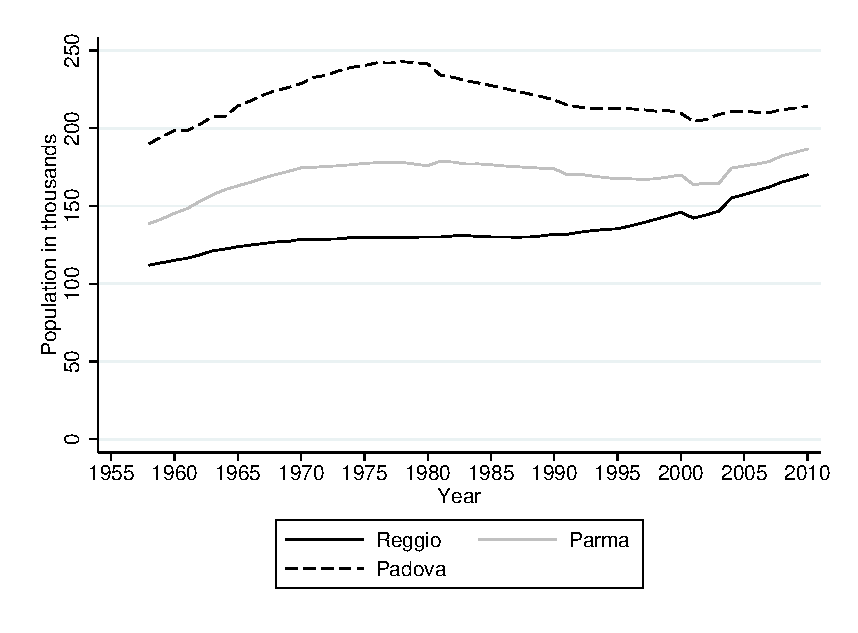
\includegraphics[width=\textwidth]{../../output/image/population.eps}       
\caption{Population}        
        \end{subfigure}
        \begin{subfigure}[t]{0.49\textwidth}
          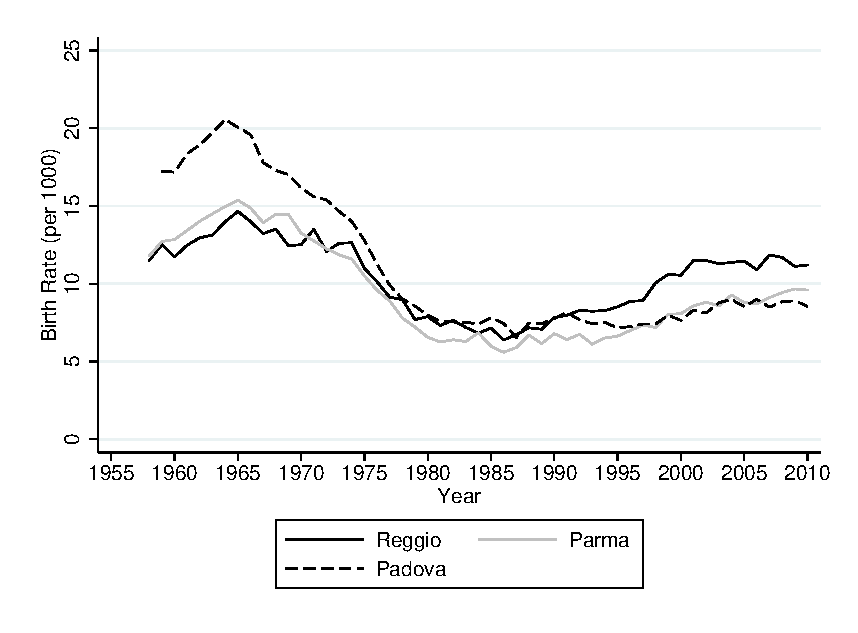
\includegraphics[width=\textwidth]{../../output/image/birth_rate.eps}       
 \caption{Birth Rate}        
        \end{subfigure}
        \begin{subfigure}[t]{0.49\textwidth}
          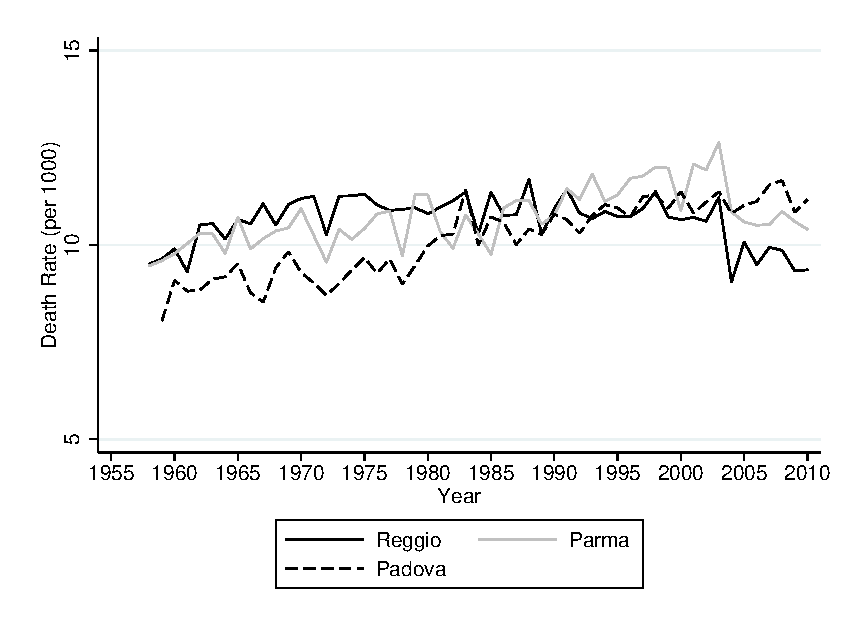
\includegraphics[width=\textwidth]{../../output/image/death_rate.eps} 
        \caption{Death Rate}        
        \end{subfigure}
        \begin{subfigure}[t]{0.49\textwidth}
          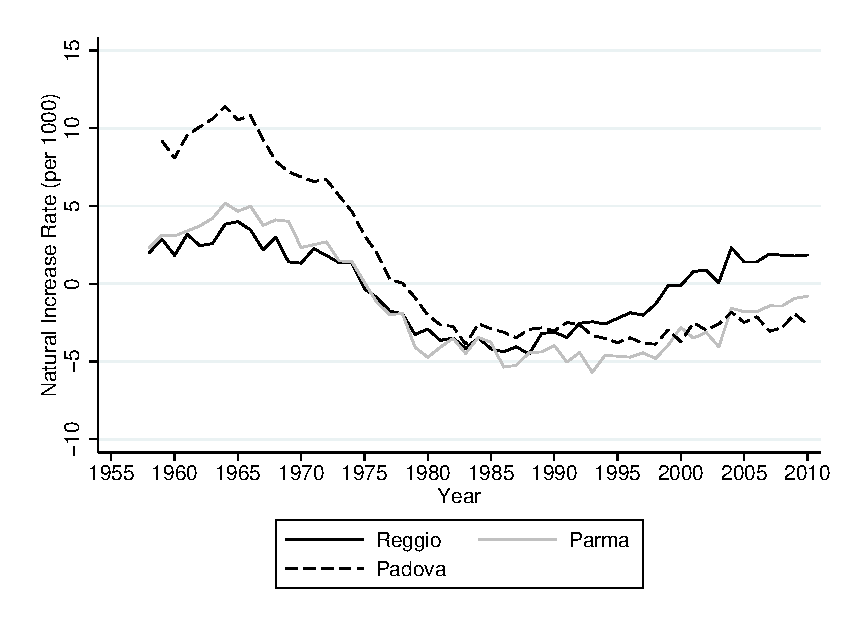
\includegraphics[width=\textwidth]{../../output/image/naturalinc_rate.eps}
            \caption{Natural Rate}       
        \end{subfigure}
      \caption{Population Statistics}  \label{fig:population}
    \end{figure}
    


\begin{figure}[H]
      \centering
        \begin{subfigure}[t]{0.49\textwidth}
          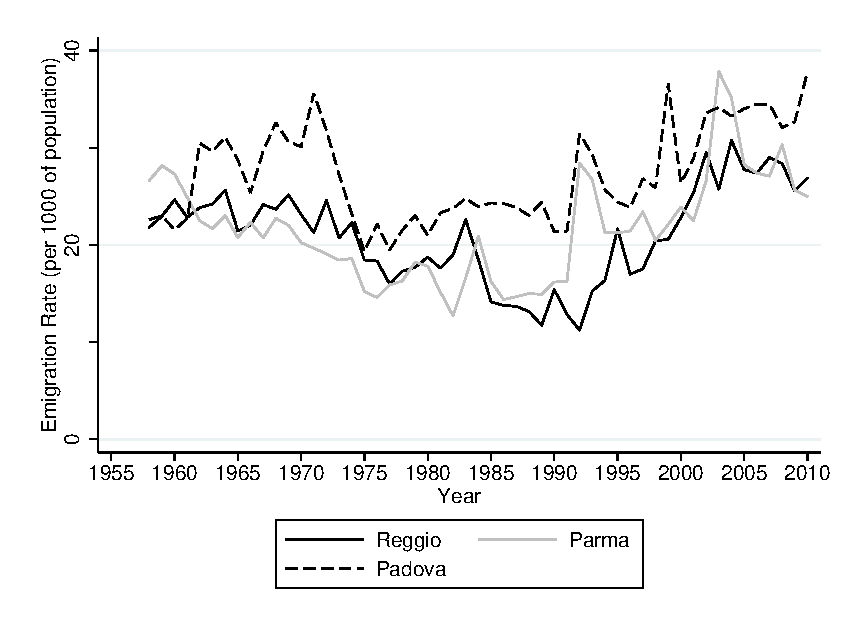
\includegraphics[width=\textwidth]{../../output/image/emigration.eps}
            \caption{Emigration}       
        \end{subfigure}
      \begin{subfigure}[t]{0.49\textwidth}
        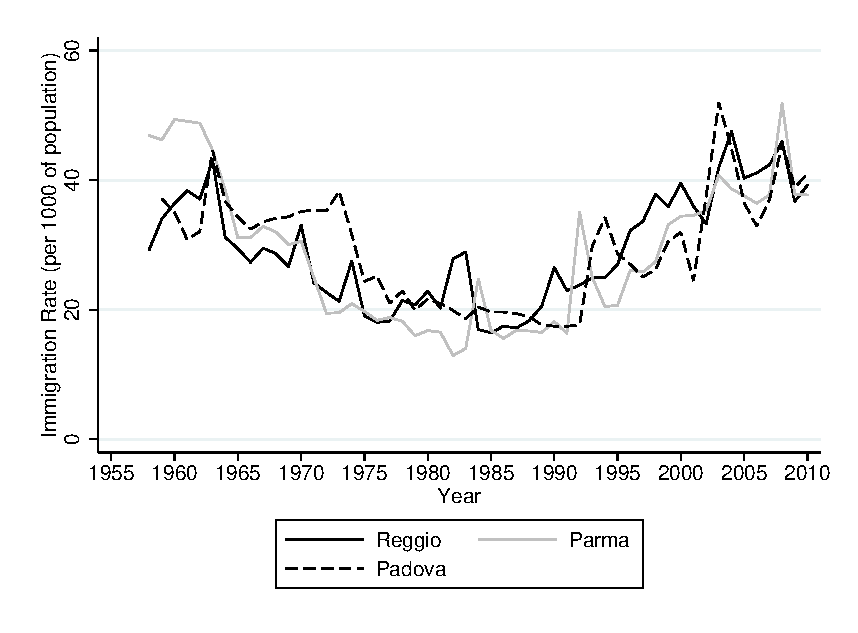
\includegraphics[width=\textwidth]{../../output/image/immigration.eps}
        \caption{Immigration}
      \end{subfigure}
	 \begin{subfigure}[t]{0.49\textwidth}
          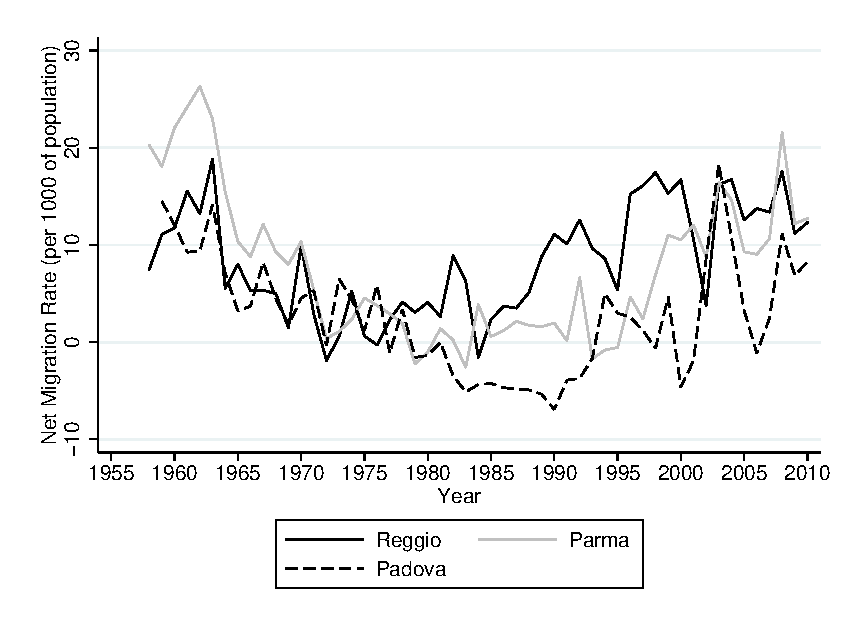
\includegraphics[width=\textwidth]{../../output/image/netmigration.eps}       
\caption{Net Migration}        
        \end{subfigure}
        \begin{subfigure}[t]{0.49\textwidth}
          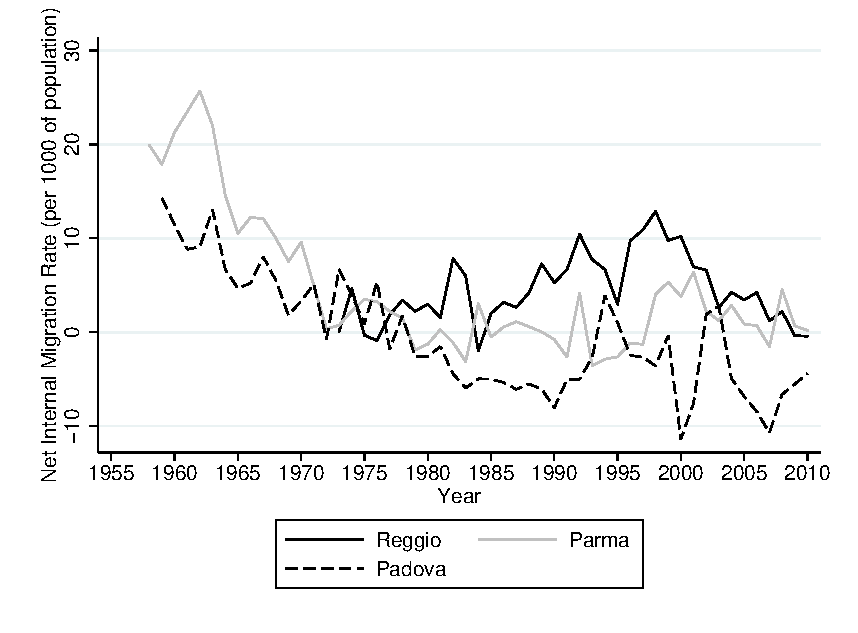
\includegraphics[width=\textwidth]{../../output/image/netinternalmig.eps}       
 \caption{Net Internal Migration}        
        \end{subfigure}
        \begin{subfigure}[ht]{0.48\textwidth}
          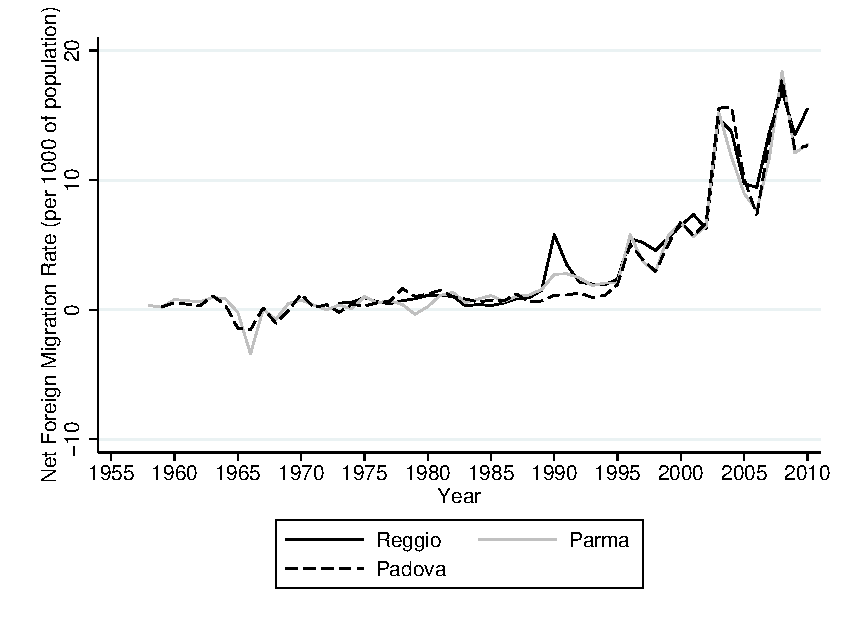
\includegraphics[width=\textwidth]{../../output/image/netforeignmig.eps} 
        \caption{Net Foreign Migration}        
        \end{subfigure}      
      
      \caption{Migration Statistics}  \label{fig:emigr-immigr}
    \end{figure}


    
    \begin{figure}[H]
      \centering
        \begin{subfigure}[t]{0.49\textwidth}
          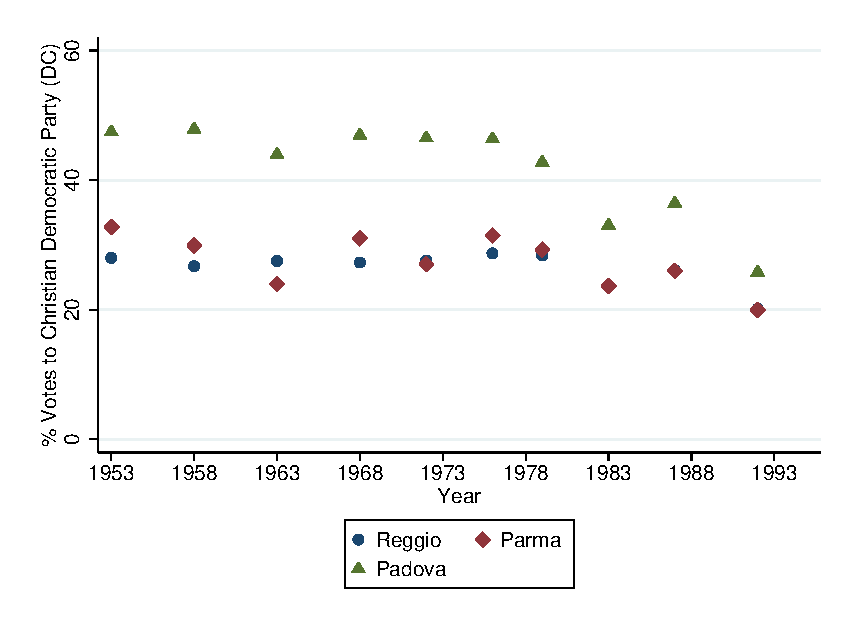
\includegraphics[width=\textwidth]{../../output/image/DC.eps}       
\caption{DC}        
        \end{subfigure}
        \begin{subfigure}[t]{0.49\textwidth}
          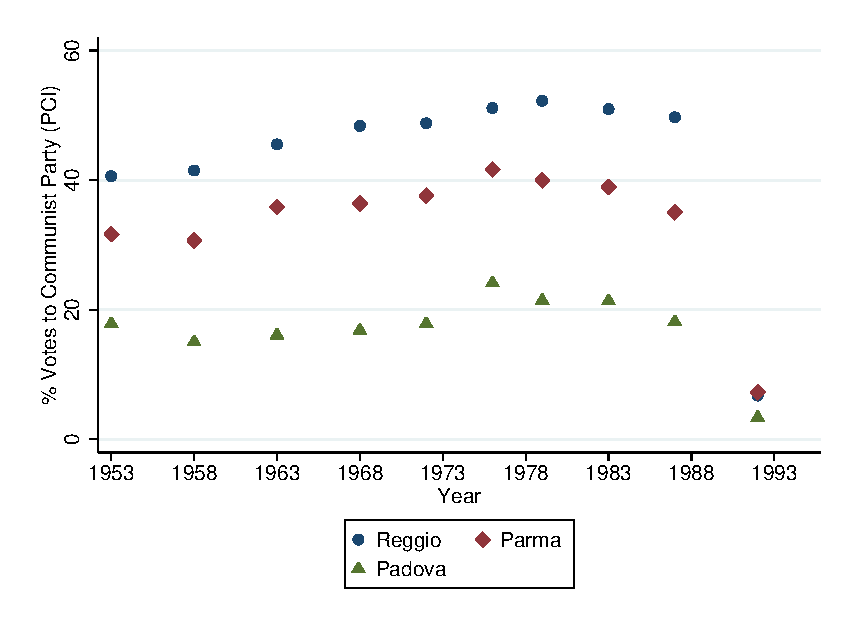
\includegraphics[width=\textwidth]{../../output/image/PCI.eps}       
 \caption{PCI}        
        \end{subfigure}
      \caption{Election Statistics}  \label{fig:election}
    \end{figure}

\section{Additional Results for Preschools (ages 3-6)}
\label{sec:results}







\subsection{Estimation Results for Reggio Approach Preschools, Comparison with Other School Types} \label{app:comparison-reli-stat}

\begin{table}[H] \caption{Estimation Results for Main Outcomes, Comparison to Religious Preschools, Child Cohort} \label{ols-M-child-reg-reli}
\scalebox{0.8}{\begin{tabular}{l c c c c c c c c c}
\toprule
 & None & BIC & Full & PSM & AIPW & DidPm & PSMPm & DidPv & PSMPv \\
\midrule
IQ Factor & \textbf{ -0.33 } & \textbf{ -0.31 } & \textbf{ -0.36 } & \textbf{-0.30} & -0.30 & 0.04 & \textbf{-0.43} & 0.14 & \textbf{-0.40} \\
& (0.10) & (0.10) & (0.11) & (0.11) & (0.09) & (0.13) & (0.14) & (0.16) & (0.10) \\
& \textit{ 314 } & \textit{ 314 } & \textit{ 314 } & \textit{ 314 } & \textit{ 314 } & \textit{ 756 } & \textit{ 291 } & \textit{ 576 } & \textit{ 375 } \\
SDQ Composite - Child & 0.67 & \textbf{ 0.84 } & \textbf{ 1.32 } & 0.21 & 0.71 & 0.16 & 0.58 & \textbf{ 1.85 } & 0.18 \\
& (0.53) & (0.52) & (0.52) & (0.55) & (0.54) & (0.66) & (0.66) & (0.81) & (0.56) \\
& \textit{ 314 } & \textit{ 314 } & \textit{ 314 } & \textit{ 314 } & \textit{ 314 } & \textit{ 755 } & \textit{ 291 } & \textit{ 576 } & \textit{ 375 } \\
Not Obese & \textbf{ -0.08 } & -0.08 & \textbf{ -0.10 } & \textbf{-0.11} & -0.08 & 0.00 & -0.09 & 0.04 & -0.05 \\
& (0.05) & (0.06) & (0.06) & (0.06) & (0.06) & (0.06) & (0.07) & (0.08) & (0.06) \\
& \textit{ 314 } & \textit{ 314 } & \textit{ 314 } & \textit{ 314 } & \textit{ 314 } & \textit{ 756 } & \textit{ 291 } & \textit{ 576 } & \textit{ 375 } \\
Not Overweight & -0.04 & -0.04 & -0.06 & -0.03 & -0.05 & -0.03 & 0.03 & -0.05 & -0.04 \\
& (0.04) & (0.04) & (0.04) & (0.05) & (0.04) & (0.05) & (0.06) & (0.05) & (0.04) \\
& \textit{ 314 } & \textit{ 314 } & \textit{ 314 } & \textit{ 314 } & \textit{ 314 } & \textit{ 756 } & \textit{ 291 } & \textit{ 576 } & \textit{ 375 } \\
Health is Good & -0.02 & -0.02 & -0.00 & -0.05 & -0.01 & 0.05 & 0.02 & -0.07 & \textbf{-0.09} \\
& (0.06) & (0.06) & (0.06) & (0.06) & (0.06) & (0.07) & (0.07) & (0.08) & (0.05) \\
& \textit{ 314 } & \textit{ 314 } & \textit{ 314 } & \textit{ 314 } & \textit{ 314 } & \textit{ 755 } & \textit{ 291 } & \textit{ 575 } & \textit{ 374 } \\
Not Excited to Learn & 0.02 & 0.02 & 0.02 & 0.02 & \textbf{0.03} & 0.01 & \textbf{-0.17} & -0.01 & 0.02 \\
& (0.02) & (0.02) & (0.02) & (0.02) & (0.02) & (0.03) & (0.06) & (0.04) & (0.02) \\
& \textit{ 314 } & \textit{ 314 } & \textit{ 314 } & \textit{ 314 } & \textit{ 314 } & \textit{ 756 } & \textit{ 291 } & \textit{ 576 } & \textit{ 375 } \\
Problems Sitting Still & -0.02 & 0.00 & -0.04 & 0.03 & 0.01 & -0.04 & 0.03 & -0.08 & 0.07 \\
& (0.04) & (0.04) & (0.04) & (0.04) & (0.04) & (0.05) & (0.04) & (0.06) & (0.04) \\
& \textit{ 314 } & \textit{ 314 } & \textit{ 314 } & \textit{ 314 } & \textit{ 314 } & \textit{ 756 } & \textit{ 291 } & \textit{ 576 } & \textit{ 375 } \\
& 0.03 & 0.02 & 0.05 & -0.00 & -0.00 & 0.07 & \textbf{-0.18} & 0.10 & \textbf{0.13} \\
& (0.07) & (0.07) & (0.08) & (0.07) & (0.06) & (0.08) & (0.06) & (0.11) & (0.07) \\
& \textit{ 313 } & \textit{ 313 } & \textit{ 313 } & \textit{ 313 } & \textit{ 313 } & \textit{ 752 } & \textit{ 291 } & \textit{ 575 } & \textit{ 375 } \\
Num. of Friends & -0.14 & -0.14 & 0.07 & 0.04 & -0.09 & -0.47 & -0.72 & 0.47 & \textbf{-1.39} \\
& (0.27) & (0.26) & (0.31) & (0.27) & (0.27) & (0.45) & (0.59) & (0.68) & (0.37) \\
& \textit{ 312 } & \textit{ 312 } & \textit{ 312 } & \textit{ 312 } & \textit{ 312 } & \textit{ 740 } & \textit{ 289 } & \textit{ 554 } & \textit{ 367 } \\
Candy Game: Willing to Share Candies & -0.01 & -0.01 & 0.00 & -0.04 & -0.00 & 0.02 & \textbf{0.10} & 0.05 & \textbf{-0.06} \\
& (0.03) & (0.04) & (0.04) & (0.03) & (0.04) & (0.04) & (0.06) & (0.05) & (0.03) \\
& \textit{ 314 } & \textit{ 314 } & \textit{ 314 } & \textit{ 314 } & \textit{ 314 } & \textit{ 756 } & \textit{ 291 } & \textit{ 576 } & \textit{ 375 } \\
\bottomrule
\end{tabular}
}
\vspace{1ex} \\
\footnotesize\raggedright{Note: This table shows the estimates of the coefficient for attending Reggio Approach preschools from multiple methods. We compare Reggio Approach people with people who attended religious preschools in Reggio. Column title indicates the corresponding control set and and model. ``NoneIt'' refers to the OLS estimate with no control variables. ``BICIt'' refers to the OLS estimate with controls selected by Bayesian Information Criterion (BIC) and additional controls for caregiver's religion. ``FullIt'' refers to the OLS estimate with the full set of controls. ``DidPmIt'' refers to the difference-in-difference estimate of (Reggio Muni - Parma Muni) - (Reggio None - Parma None). ``DidPvIt'' refers to the difference-in-difference estimate of (Reggio Muni - Padova Muni) - (Reggio None - Padova None). ``AIPWIt" refers to AIPW estimate for comparing Reggio Approach children with children in Reggio who attended other type of preschool. Robust standard errors are reported in parentheses. Bold number shows that the estimate is statistically significant at the 10\% level. Number of observations used in estimation is reported in italic.}

\end{table}


\begin{table}[H] \caption{Estimation Results for Main Outcomes, Comparison to State Preschools, Child Cohort} \label{ols-M-child-reg-state}
\scalebox{0.8}{\begin{tabular}{l c c c c c c c c c}
\toprule
 & None & BIC & Full & PSM & AIPW & DidPm & PSMPm & DidPv & PSMPv \\
\midrule
IQ Factor & \textbf{ 0.28 } & 0.21 & 0.17 & 0.25 & 0.11 & 0.04 & \textbf{-0.56} & 0.15 & 0.08 \\
& (0.14) & (0.15) & (0.15) & (0.17) & (0.14) & (0.13) & (0.11) & (0.20) & (0.17) \\
& \textit{ 291 } & \textit{ 291 } & \textit{ 291 } & \textit{ 291 } & \textit{ 291 } & \textit{ 756 } & \textit{ 264 } & \textit{ 476 } & \textit{ 302 } \\
SDQ Composite - Child & 0.80 & 0.69 & 0.97 & 0.84 & 0.67 & 0.16 & -0.43 & 0.43 & \textbf{1.69} \\
& (0.69) & (0.72) & (0.68) & (0.73) & (0.70) & (0.66) & (0.64) & (0.99) & (0.84) \\
& \textit{ 291 } & \textit{ 291 } & \textit{ 291 } & \textit{ 291 } & \textit{ 291 } & \textit{ 755 } & \textit{ 264 } & \textit{ 476 } & \textit{ 302 } \\
Not Obese & 0.09 & 0.00 & 0.04 & -0.01 & -0.02 & 0.00 & \textbf{-0.24} & 0.03 & -0.00 \\
& (0.06) & (0.07) & (0.06) & (0.07) & (0.07) & (0.06) & (0.05) & (0.10) & (0.07) \\
& \textit{ 291 } & \textit{ 291 } & \textit{ 291 } & \textit{ 291 } & \textit{ 291 } & \textit{ 756 } & \textit{ 264 } & \textit{ 476 } & \textit{ 302 } \\
Not Overweight & \textbf{ -0.06 } & -0.05 & -0.06 & -0.05 & -0.03 & -0.03 & -0.02 & \textbf{ -0.16 } & -0.01 \\
& (0.04) & (0.05) & (0.05) & (0.06) & (0.05) & (0.05) & (0.04) & (0.07) & (0.08) \\
& \textit{ 291 } & \textit{ 291 } & \textit{ 291 } & \textit{ 291 } & \textit{ 291 } & \textit{ 756 } & \textit{ 264 } & \textit{ 476 } & \textit{ 302 } \\
Health is Good & -0.07 & -0.04 & 0.00 & -0.08 & -0.02 & 0.05 & 0.03 & 0.00 & \textbf{-0.18} \\
& (0.06) & (0.07) & (0.07) & (0.08) & (0.07) & (0.07) & (0.07) & (0.08) & (0.06) \\
& \textit{ 291 } & \textit{ 291 } & \textit{ 291 } & \textit{ 291 } & \textit{ 291 } & \textit{ 755 } & \textit{ 264 } & \textit{ 476 } & \textit{ 302 } \\
Not Excited to Learn & -0.04 & -0.03 & -0.03 & -0.01 & -0.02 & 0.01 & -0.04 & -0.07 & -0.00 \\
& (0.03) & (0.04) & (0.04) & (0.03) & (0.03) & (0.03) & (0.05) & (0.05) & (0.03) \\
& \textit{ 291 } & \textit{ 291 } & \textit{ 291 } & \textit{ 291 } & \textit{ 291 } & \textit{ 756 } & \textit{ 264 } & \textit{ 476 } & \textit{ 302 } \\
Problems Sitting Still & 0.05 & 0.06 & 0.04 & 0.06 & \textbf{0.05} & -0.04 & 0.02 & -0.04 & 0.04 \\
& (0.04) & (0.05) & (0.05) & (0.04) & (0.04) & (0.05) & (0.06) & (0.06) & (0.05) \\
& \textit{ 291 } & \textit{ 291 } & \textit{ 291 } & \textit{ 291 } & \textit{ 291 } & \textit{ 756 } & \textit{ 264 } & \textit{ 476 } & \textit{ 302 } \\
How Much Child Likes School & -0.01 & -0.09 & -0.04 & 0.05 & -0.07 & 0.07 & -0.09 & 0.10 & -0.02 \\
& (0.08) & (0.08) & (0.09) & (0.14) & (0.08) & (0.08) & (0.10) & (0.12) & (0.11) \\
& \textit{ 291 } & \textit{ 291 } & \textit{ 291 } & \textit{ 291 } & \textit{ 291 } & \textit{ 752 } & \textit{ 264 } & \textit{ 476 } & \textit{ 302 } \\
Num. of Friends & -0.22 & -0.47 & -0.36 & -0.39 & -0.40 & -0.47 & 0.96 & \textbf{ -1.02 } & -0.06 \\
& (0.32) & (0.38) & (0.42) & (0.51) & (0.42) & (0.45) & (0.62) & (0.70) & (0.49) \\
& \textit{ 287 } & \textit{ 287 } & \textit{ 287 } & \textit{ 287 } & \textit{ 287 } & \textit{ 740 } & \textit{ 264 } & \textit{ 450 } & \textit{ 291 } \\
Candy Game: Willing to Share Candies & 0.02 & 0.01 & -0.00 & -0.03 & -0.00 & 0.02 & 0.02 & 0.07 & \textbf{-0.08} \\
& (0.04) & (0.04) & (0.05) & (0.04) & (0.04) & (0.04) & (0.08) & (0.06) & (0.03) \\
& \textit{ 291 } & \textit{ 291 } & \textit{ 291 } & \textit{ 291 } & \textit{ 291 } & \textit{ 756 } & \textit{ 264 } & \textit{ 476 } & \textit{ 302 } \\
\bottomrule
\end{tabular}
}
\vspace{1ex} \\
\footnotesize\raggedright{Note: This table shows the estimates of the coefficient for attending Reggio Approach preschools from multiple methods. We compare Reggio Approach people with people who attended State preschools in Reggio. Column title indicates the corresponding control set and and model. ``NoneIt'' refers to the OLS estimate with no control variables. ``BICIt'' refers to the OLS estimate with controls selected by Bayesian Information Criterion (BIC) and additional controls for caregiver's religion. ``FullIt'' refers to the OLS estimate with the full set of controls. ``DidPmIt'' refers to the difference-in-difference estimate of (Reggio Muni - Parma Muni) - (Reggio None - Parma None). ``DidPvIt'' refers to the difference-in-difference estimate of (Reggio Muni - Padova Muni) - (Reggio None - Padova None). ``AIPWIt" refers to AIPW estimate for comparing Reggio Approach children with children in Reggio who did not attend any preschool. Robust standard errors are reported in parentheses. Bold number shows that the estimate is statistically significant at the 10\% level. Number of observations used in estimation is reported in italic.}

\end{table}


\begin{table}[H] \caption{Estimation Results for Main Outcomes, Comparison to Religious Preschools, Adolescent Cohort} \label{ols-M-adol-reg-reli}
\scalebox{0.8}{\begin{tabular}{l c c c c c c}
\toprule
 & None & Bic & Full & AIPW & DidPm & DidPv \\
\midrule
IQ Score &     -0.03 &     -0.04 &     -0.01 &     -0.06 &     -0.03 &     -0.01 \\
& (     0.03 ) & (     0.04 ) & (     0.03 ) & (     0.03 ) & (     0.06 ) & (     0.05 ) \\
& \textit{ 252 } & \textit{ 252 } & \textit{ 252 } & \textit{ 252 } & \textit{ 377 } & \textit{ 469 } \\
IQ Factor &     -0.12 & \textbf{     -0.18 } &     -0.06 &     -0.23 &     -0.05 &     -0.05 \\
& (     0.10 ) & (     0.12 ) & (     0.11 ) & (     0.12 ) & (     0.18 ) & (     0.18 ) \\
& \textit{ 252 } & \textit{ 252 } & \textit{ 252 } & \textit{ 252 } & \textit{ 377 } & \textit{ 469 } \\
SDQ Composite - Child &      0.50 &      0.44 & \textbf{      1.18 } &      0.61 &      0.25 &      0.09 \\
& (     0.70 ) & (     0.83 ) & (     0.76 ) & (     0.91 ) & (     1.28 ) & (     0.92 ) \\
& \textit{ 252 } & \textit{ 252 } & \textit{ 252 } & \textit{ 252 } & \textit{ 377 } & \textit{ 465 } \\
SDQ Composite & \textbf{      1.42 } & \textbf{      1.67 } & \textbf{      1.51 } & \textbf{     1.57} &      1.65 &      0.80 \\
& (     0.69 ) & (     0.80 ) & (     0.81 ) & (     0.85 ) & (     1.20 ) & (     1.04 ) \\
& \textit{ 250 } & \textit{ 250 } & \textit{ 250 } & \textit{ 250 } & \textit{ 374 } & \textit{ 465 } \\
Depression Score - positive & \textbf{      1.81 } & \textbf{      2.25 } & \textbf{      2.25 } & \textbf{     2.66} & \textbf{      2.29 } &      1.49 \\
& (     0.88 ) & (     0.98 ) & (     1.02 ) & (     1.09 ) & (     1.35 ) & (     1.26 ) \\
& \textit{ 246 } & \textit{ 246 } & \textit{ 246 } & \textit{ 246 } & \textit{ 365 } & \textit{ 461 } \\
Locus of Control - positive &      0.07 &      0.09 &      0.08 &      0.09 &     -0.12 &      0.15 \\
& (     0.09 ) & (     0.11 ) & (     0.10 ) & (     0.14 ) & (     0.17 ) & (     0.14 ) \\
& \textit{ 249 } & \textit{ 249 } & \textit{ 249 } & \textit{ 249 } & \textit{ 372 } & \textit{ 464 } \\
Obese & \textbf{      0.11 } & \textbf{      0.12 } & \textbf{      0.10 } & \textbf{     0.12} &     -0.01 &      0.05 \\
& (     0.04 ) & (     0.05 ) & (     0.05 ) & (     0.05 ) & (     0.08 ) & (     0.07 ) \\
& \textit{ 252 } & \textit{ 252 } & \textit{ 252 } & \textit{ 252 } & \textit{ 377 } & \textit{ 469 } \\
Overweight &     -0.00 &      0.01 &      0.01 &      0.00 & \textbf{     -0.11 } &      0.03 \\
& (     0.02 ) & (     0.03 ) & (     0.03 ) & (     0.03 ) & (     0.06 ) & (     0.03 ) \\
& \textit{ 252 } & \textit{ 252 } & \textit{ 252 } & \textit{ 252 } & \textit{ 377 } & \textit{ 469 } \\
Health is Good &      0.04 &      0.06 &      0.06 &      0.06 & \textbf{      0.19 } &      0.07 \\
& (     0.06 ) & (     0.07 ) & (     0.07 ) & (     0.07 ) & (     0.12 ) & (     0.09 ) \\
& \textit{ 251 } & \textit{ 251 } & \textit{ 251 } & \textit{ 251 } & \textit{ 376 } & \textit{ 468 } \\
Go To School &      0.03 &      0.00 &      0.02 &     -0.01 &      0.00 & \textbf{      0.04 } \\
& (     0.03 ) & (     0.02 ) & (     0.03 ) & (     0.02 ) & (     0.03 ) & (     0.03 ) \\
& \textit{ 252 } & \textit{ 252 } & \textit{ 252 } & \textit{ 252 } & \textit{ 377 } & \textit{ 469 } \\
How Much Child Likes School &     -0.10 &     -0.08 &     -0.14 &      0.04 &      0.02 &     -0.09 \\
& (     0.12 ) & (     0.14 ) & (     0.13 ) & (     0.14 ) & (     0.21 ) & (     0.17 ) \\
& \textit{ 241 } & \textit{ 241 } & \textit{ 241 } & \textit{ 241 } & \textit{ 363 } & \textit{ 455 } \\
Days of Sport (Weekly) &     -0.23 &     -0.19 &     -0.03 &     -0.33 &     -0.45 &     -0.32 \\
& (     0.25 ) & (     0.29 ) & (     0.29 ) & (     0.32 ) & (     0.44 ) & (     0.37 ) \\
& \textit{ 247 } & \textit{ 247 } & \textit{ 247 } & \textit{ 247 } & \textit{ 368 } & \textit{ 451 } \\
\bottomrule
\end{tabular}
}
\vspace{1ex} \\
\footnotesize\raggedright{Note: This table shows the estimates of the coefficient for attending Reggio Approach preschools from multiple methods. We compare Reggio Approach people with people who attended religious preschools in Reggio. Column title indicates the corresponding control set and and model. ``None'' refers to the OLS estimate with no control variables. ``BIC'' refers to the OLS estimate with controls selected by Bayesian Information Criterion (BIC) and additional controls for caregiver's religion. ``Full'' refers to the OLS estimate with the full set of controls. ``DidPm'' refers to the difference-in-difference estimate of (Reggio Muni - Parma Muni) - (Reggio None - Parma None). ``DidPv'' refers to the difference-in-difference estimate of (Reggio Muni - Padova Muni) - (Reggio None - Padova None). ``AIPW" refers to AIPW estimate for comparing Reggio Approach children with children in Reggio who attended other type of preschool. Robust standard errors are reported in parentheses. Bold number shows that the estimate is statistically significant at the 10\% level. Number of observations used in estimation is reported in italic.}
\end{table}

\begin{table}[H] \caption{Estimation Results for Main Outcomes, Comparison to State Preschools, Adolescent Cohort} \label{ols-M-adol-reg-stat}
\scalebox{0.8}{\begin{tabular}{l c c c c c c}
\toprule
 & None & Bic & Full & DidPm & DidPv & AIPW \\
\midrule
SDQ Composite - Child & \textbf{     -2.13 } & \textbf{     -1.92 } & \textbf{     -1.70 } & \textbf{     -1.51 } &      0.09 &     -1.11 \\
& (     0.62 ) & (     0.69 ) & (     0.69 ) & (     0.84 ) & (     0.72 ) & (     0.91 ) \\
SDQ Composite &     -1.03 &     -1.18 &     -1.36 & \textbf{     -1.88 } & \textbf{     -1.52 } &     -2.22 \\
& (     1.00 ) & (     1.03 ) & (     1.11 ) & (     0.99 ) & (     0.78 ) & (     1.25 ) \\
Depression Score - positive &      0.01 &      0.19 &      0.22 & \textbf{     -2.25 } & \textbf{     -2.57 } &     -1.51 \\
& (     1.25 ) & (     1.31 ) & (     1.43 ) & (     1.00 ) & (     0.93 ) & (     1.42 ) \\
Obese &     -0.03 &      0.02 &      0.01 &      0.08 & \textbf{     -0.22 } &     -0.06 \\
& (     0.08 ) & (     0.09 ) & (     0.08 ) & (     0.06 ) & (     0.08 ) & (     0.13 ) \\
Overweight &     -0.04 &     -0.03 &     -0.02 &      0.05 &     -0.02 &      0.03 \\
& (     0.05 ) & (     0.05 ) & (     0.05 ) & (     0.05 ) & (     0.02 ) & (     0.04 ) \\
Health is Good &      0.05 &      0.09 &      0.10 & \textbf{      0.13 } & \textbf{     -0.13 } &      0.08 \\
& (     0.10 ) & (     0.10 ) & (     0.11 ) & (     0.09 ) & (     0.07 ) & (     0.14 ) \\
Go To School &      0.05 &      0.03 &      0.04 &      0.00 &      0.01 &      0.04 \\
& (     0.05 ) & (     0.05 ) & (     0.06 ) & (     0.01 ) & (     0.02 ) & (     0.08 ) \\
How Much Child Likes School &     -0.26 & \textbf{     -0.38 } & \textbf{     -0.44 } & \textbf{     -0.39 } &     -0.15 &     -0.16 \\
& (     0.20 ) & (     0.21 ) & (     0.20 ) & (     0.18 ) & (     0.16 ) & (     0.35 ) \\
Trust Score &      0.21 &      0.05 &      0.05 & \textbf{     -0.60 } &      0.17 &      0.23 \\
& (     0.31 ) & (     0.33 ) & (     0.31 ) & (     0.28 ) & (     0.25 ) & (     0.38 ) \\
Days of Sport (Weekly) & \textbf{     -0.84 } & \textbf{     -0.92 } & \textbf{     -0.90 } &      0.48 &     -0.02 &     -1.28 \\
& (     0.38 ) & (     0.41 ) & (     0.43 ) & (     0.34 ) & (     0.34 ) & (     0.62 ) \\
\bottomrule
\end{tabular}
}
\vspace{1ex} \\
\footnotesize\raggedright{Note: This table shows the estimates of the coefficient for attending Reggio Approach preschools from multiple methods. We compare Reggio Approach people with people who attended state preschools in Reggio. Column title indicates the corresponding control set and and model. ``None'' refers to the OLS estimate with no control variables. ``BIC'' refers to the OLS estimate with controls selected by Bayesian Information Criterion (BIC) and additional controls for caregiver's religion. ``Full'' refers to the OLS estimate with the full set of controls. ``DidPm'' refers to the difference-in-difference estimate of (Reggio Muni - Parma Muni) - (Reggio None - Parma None). ``DidPv'' refers to the difference-in-difference estimate of (Reggio Muni - Padova Muni) - (Reggio None - Padova None).  ``AIPW" refers to AIPW estimate for comparing Reggio Approach children with children in Reggio who did not attend any preschool. Robust standard errors are reported in parentheses. Bold number shows that the estimate is statistically significant at the 10\% level. Number of observations used in estimation is reported in italic.}
\end{table}




\begin{table}[H] \caption{Estimation Results for Main Outcomes, Comparison to Religious Preschools, Adult Cohorts} \label{ols-M-adult-reg-reli}
\scalebox{0.75}{\begin{tabular}{l c c c c c c c c c c}
\toprule
 & None30 & BIC30 & Full30 & DidPm30 & DidPv30 & None40 & BIC40 & Full40 & AIPW30 & AIPW40 \\
\midrule
Graduate from High School &     -0.01 &     -0.00 &     -0.02 & \textbf{     -0.16 } & \textbf{      0.09 } &      0.09 &      0.08 &      0.09 &     -0.00 & \textbf{     0.07} \\
& (     0.06) & (     0.06) & (     0.07) & (     0.07) & (     0.06) & (     0.08) & (     0.08) & (     0.08) & (     0.07) & (     0.07) \\
Max Edu: University & \textbf{      0.11 } &      0.10 &      0.08 & \textbf{     -0.24 } &     -0.12 &      0.08 &      0.06 &      0.04 &      0.08 &      0.04 \\
& (     0.07) & (     0.07) & (     0.09) & (     0.10) & (     0.12) & (     0.06) & (     0.06) & (     0.06) & (     0.10) & (     0.06) \\
Employed & \textbf{     -0.05 } & \textbf{     -0.06 } &     -0.03 &     -0.08 &      0.03 &     -0.01 &      0.00 &     -0.01 &     -0.06 &      0.02 \\
& (     0.02) & (     0.03) & (     0.02) & (     0.07) & (     0.09) & (     0.03) & (     0.04) & (     0.04) & (     0.02) & (     0.04) \\
Hours Worked Per Week & \textbf{      1.96 } & \textbf{      1.80 } &      0.92 &      1.19 &     -1.42 &     -1.25 &     -2.25 & \textbf{     -2.41 } & \textbf{     1.53} &     -1.98 \\
& (     1.09) & (     1.14) & (     1.31) & (     2.27) & (     1.36) & (     1.43) & (     1.59) & (     1.60) & (     1.20) & (     1.83) \\
Married or Cohabitating &      0.01 &      0.01 &      0.04 &     -0.08 &     -0.15 &      0.01 &      0.02 &      0.02 &     -0.04 &      0.01 \\
& (     0.09) & (     0.10) & (     0.11) & (     0.11) & (     0.12) & (     0.08) & (     0.08) & (     0.08) & (     0.10) & (     0.09) \\
Obese & \textbf{      0.11 } & \textbf{      0.14 } &      0.09 & \textbf{     -0.17 } &     -0.03 &      0.10 &      0.09 &      0.04 & \textbf{     0.13} & \textbf{     0.09} \\
& (     0.07) & (     0.07) & (     0.09) & (     0.09) & (     0.10) & (     0.08) & (     0.07) & (     0.08) & (     0.09) & (     0.08) \\
Overweight &     -0.01 &     -0.02 &      0.01 & \textbf{      0.18 } &     -0.01 &     -0.07 &     -0.06 &     -0.04 &     -0.02 &     -0.03 \\
& (     0.08) & (     0.08) & (     0.08) & (     0.09) & (     0.09) & (     0.09) & (     0.08) & (     0.08) & (     0.09) & (     0.07) \\
Locus of Control - positive &     -0.10 &     -0.08 &     -0.10 &     -0.18 & \textbf{     -0.30 } &      0.01 &      0.01 &     -0.04 &     -0.07 &     -0.01 \\
& (     0.15) & (     0.14) & (     0.17) & (     0.22) & (     0.20) & (     0.14) & (     0.15) & (     0.16) & (     0.16) & (     0.16) \\
&     -1.50 & \textbf{     -1.50 } &     -1.23 &     -0.13 &     -1.45 &      0.26 &      1.03 &      0.69 &     -1.50 &      1.00 \\
& (     1.10) & (     0.83) & (     0.89) & (     1.15) & (     1.61) & (     0.93) & (     0.90) & (     0.97) & (     0.93) & (     1.01) \\
Ever Voted for Municipal &     -0.06 &     -0.01 &     -0.01 &     -0.09 & \textbf{     -0.25 } &      0.00 &      0.11 &      0.11 &      0.04 & \textbf{     0.12} \\
& (     0.10) & (     0.07) & (     0.10) & (     0.08) & (     0.10) & (     0.09) & (     0.08) & (     0.08) & (     0.07) & (     0.08) \\
Ever Voted for Regional &     -0.06 &     -0.01 &     -0.02 &     -0.07 & \textbf{     -0.34 } &      0.04 & \textbf{      0.15 } & \textbf{      0.13 } &      0.01 & \textbf{     0.15} \\
& (     0.10) & (     0.07) & (     0.09) & (     0.08) & (     0.09) & (     0.09) & (     0.08) & (     0.08) & (     0.06) & (     0.07) \\
\bottomrule
\end{tabular}
}
\vspace{1ex} \\
\footnotesize\raggedright{Note: This table shows the estimates of the coefficient for attending Reggio Approach preschools from multiple methods. We compare Reggio Approach people with people who attended religious preschools in Reggio.  Column title indicates the corresponding control set and and model. For age-30 cohort, the columns are as follows: ``None30'' refers to the OLS estimate with no control variables. ``BIC30'' refers to the OLS estimate with controls selected by Bayesian Information Criterion (BIC) and additional controls for caregiver's religion. ``Full30'' refers to the OLS estimate with the full set of controls. ``DidPm30'' refers to the difference-in-difference estimate of (Reggio Muni - Parma Muni) - (Reggio None - Parma None). ``DidPv30'' refers to the difference-in-difference estimate of (Reggio Muni - Padova Muni) - (Reggio None - Padova None).  ``AIPW30" refers to AIPW estimate for comparing Reggio Approach children with children in Reggio who attended other type of preschool. Column titles are analogous for age-40 cohort. Robust standard errors are reported in parentheses. Bold number shows that the estimate is statistically significant at the 10\% level. Number of observations used in estimation is reported in italic.}
\end{table}

\begin{table}[H] \caption{Estimation Results for Main Outcomes, Comparison to State Preschools, Adult Cohorts} \label{ols-M-adult-reg-stat}
\scalebox{0.75}{\begin{tabular}{l c c c c c c c c c c}
\toprule
 & None30 & BIC30 & Full30 & DidPm30 & DidPv30 & AIPW30 & None40 & BIC40 & Full40 & AIPW40 \\
\midrule
Graduate from High School & \textbf{     -0.13 } & \textbf{     -0.08 } & \textbf{     -0.10 } & \textbf{     -0.16 } &      0.03 &     -0.11 &     -0.01 &     -0.05 &     -0.07 &     -0.06 \\
& (     0.03 ) & (     0.03 ) & (     0.05 ) & (     0.07 ) & (     0.08 ) & (     0.03 ) & (     0.10 ) & (     0.09 ) & (     0.11 ) & (     0.15 ) \\
Max Edu: University &     -0.08 &     -0.03 &     -0.00 &     -0.12 &     -0.16 &     -0.07 &      0.05 &      0.04 &      0.02 & \textbf{     0.22} \\
& (     0.11 ) & (     0.11 ) & (     0.11 ) & (     0.10 ) & (     0.17 ) & (     0.13 ) & (     0.10 ) & (     0.10 ) & (     0.11 ) & (     0.17 ) \\
Employed &      0.03 &      0.02 &     -0.01 & \textbf{     -0.09 } &     -0.11 &      0.05 &      0.04 &      0.02 &      0.05 &      0.06 \\
& (     0.06 ) & (     0.07 ) & (     0.06 ) & (     0.06 ) & (     0.08 ) & (     0.06 ) & (     0.07 ) & (     0.07 ) & (     0.09 ) & (     0.11 ) \\
Hours Worked Per Week & \textbf{      3.03 } & \textbf{      2.84 } & \textbf{      3.11 } &      0.94 &      0.48 & \textbf{     3.13} &     -2.36 &     -0.79 &     -2.69 &     -3.73 \\
& (     0.82 ) & (     0.95 ) & (     1.04 ) & (     2.28 ) & (     2.01 ) & (     0.73 ) & (     1.87 ) & (     2.18 ) & (     2.45 ) & (     3.21 ) \\
Married or Cohabitating & \textbf{      0.18 } &      0.06 &      0.01 &     -0.10 &      0.02 &      0.06 &      0.12 &      0.10 &      0.17 &     -0.27 \\
& (     0.09 ) & (     0.09 ) & (     0.10 ) & (     0.11 ) & (     0.17 ) & (     0.12 ) & (     0.14 ) & (     0.14 ) & (     0.15 ) & (     0.28 ) \\
Obese & \textbf{     -0.22 } &     -0.07 &     -0.06 &     -0.01 &      0.08 &     -0.07 & \textbf{     -0.27 } & \textbf{     -0.30 } & \textbf{     -0.28 } &     -0.54 \\
& (     0.11 ) & (     0.07 ) & (     0.08 ) & (     0.08 ) & (     0.13 ) & (     0.07 ) & (     0.14 ) & (     0.13 ) & (     0.14 ) & (     0.25 ) \\
Overweight &      0.09 &     -0.01 &     -0.04 &      0.13 &      0.09 &      0.07 & \textbf{      0.20 } & \textbf{      0.19 } &      0.14 & \textbf{     0.33} \\
& (     0.08 ) & (     0.09 ) & (     0.09 ) & (     0.10 ) & (     0.11 ) & (     0.09 ) & (     0.08 ) & (     0.10 ) & (     0.11 ) & (     0.20 ) \\
Locus of Control - positive & \textbf{      0.41 } &      0.18 &      0.18 &      0.22 &      0.26 & \textbf{     0.22} & \textbf{      0.49 } & \textbf{      0.74 } & \textbf{      0.72 } & \textbf{     1.06} \\
& (     0.15 ) & (     0.14 ) & (     0.15 ) & (     0.23 ) & (     0.26 ) & (     0.15 ) & (     0.29 ) & (     0.25 ) & (     0.28 ) & (     0.54 ) \\
& \textbf{      3.36 } &      0.71 &      0.99 &     -1.45 &      2.39 &      0.29 &      1.82 &      2.75 &      2.40 &      2.64 \\
& (     1.61 ) & (     0.95 ) & (     1.00 ) & (     1.34 ) & (     2.20 ) & (     0.94 ) & (     2.11 ) & (     2.06 ) & (     2.29 ) & (     2.57 ) \\
Ever Voted for Municipal &      0.16 &      0.04 &      0.08 &      0.01 & \textbf{     -0.43 } &      0.04 &     -0.04 &      0.09 &     -0.04 &      0.16 \\
& (     0.12 ) & (     0.10 ) & (     0.10 ) & (     0.07 ) & (     0.12 ) & (     0.13 ) & (     0.15 ) & (     0.15 ) & (     0.17 ) & (     0.26 ) \\
Ever Voted for Regional &      0.07 &     -0.05 &      0.01 &     -0.03 & \textbf{     -0.52 } &     -0.05 &     -0.09 &      0.03 &     -0.05 &      0.09 \\
& (     0.12 ) & (     0.11 ) & (     0.11 ) & (     0.07 ) & (     0.12 ) & (     0.12 ) & (     0.14 ) & (     0.16 ) & (     0.17 ) & (     0.26 ) \\
\bottomrule
\end{tabular}
}
\vspace{1ex} \\
\footnotesize\raggedright{Note: This table shows the estimates of the coefficient for attending Reggio Approach preschools from multiple methods. We compare Reggio Approach people with people who attended state preschool in Reggio. Column title indicates the corresponding control set and and model. For age-30 cohort, the columns are as follows: ``None30'' refers to the OLS estimate with no control variables. ``BIC30'' refers to the OLS estimate with controls selected by Bayesian Information Criterion (BIC) and additional controls for caregiver's religion. ``Full30'' refers to the OLS estimate with the full set of controls. ``DidPm30'' refers to the difference-in-difference estimate of (Reggio Muni - Parma Muni) - (Reggio None - Parma None). ``DidPv30'' refers to the difference-in-difference estimate of (Reggio Muni - Padova Muni) - (Reggio None - Padova None).  ``AIPW30" refers to AIPW estimate for comparing Reggio Approach children with children in Reggio who did not attend any preschool. Column titles are analogous for age-40 cohort. Robust standard errors are reported in parentheses. Bold number shows that the estimate is statistically significant at the 10\% level. Number of observations used in estimation is reported in italic.}
\end{table}











\subsection{Estimation Results for Preschools in Parma}

% ========================================================================= %
% CHILD COHORT


\begin{table}[H] \caption{Estimation Results for Main Outcomes, Preschool vs. No Preschool, Child Cohort in Parma} \label{ols-M-child-reg-pres-parma}
\scalebox{0.8}{\begin{tabular}{l c c c c}
\toprule
 & NoneIt & BICIt & FullIt \\
\midrule
SDQ Composite - Child &      1.41 &      1.40 &      1.52 \\
& (     1.22 ) & (     1.63 ) & (     1.57 ) \\
& \textit{ 163 } & \textit{ 163 } & \textit{ 163 } \\
Obese & \textbf{     -0.40 } &     -0.15 &     -0.32 \\
& (     0.20 ) & (     0.23 ) & (     0.24 ) \\
& \textit{ 163 } & \textit{ 163 } & \textit{ 163 } \\
Overweight &     -0.03 &      0.05 &      0.22 \\
& (     0.16 ) & (     0.24 ) & (     0.28 ) \\
& \textit{ 163 } & \textit{ 163 } & \textit{ 163 } \\
Health is Good & \textbf{      0.29 } & \textbf{      0.38 } &      0.21 \\
& (     0.20 ) & (     0.24 ) & (     0.26 ) \\
& \textit{ 163 } & \textit{ 163 } & \textit{ 163 } \\
Not Excited to Learn & \textbf{      0.04 } &      0.07 &      0.02 \\
& (     0.02 ) & (     0.06 ) & (     0.05 ) \\
& \textit{ 163 } & \textit{ 163 } & \textit{ 163 } \\
Problems Sitting Still & \textbf{      0.15 } & \textbf{      0.20 } & \textbf{      0.34 } \\
& (     0.03 ) & (     0.11 ) & (     0.13 ) \\
& \textit{ 163 } & \textit{ 163 } & \textit{ 163 } \\
How Much Child Likes School &      0.40 & \textbf{      0.44 } & \textbf{      0.61 } \\
& (     0.31 ) & (     0.27 ) & (     0.25 ) \\
& \textit{ 161 } & \textit{ 161 } & \textit{ 161 } \\
\bottomrule
\end{tabular}
}
\vspace{1ex} \\
\footnotesize\raggedright{Note: This table shows the estimates of the coefficient for attending preschools in Parma from multiple methods. We compare people in Parma who attended preschools with people in Parma who attended no preschools. Column title indicates the corresponding control set and and model. ``NoneIt'' refers to the OLS estimate with no control variables. ``BICIt'' refers to the OLS estimate with controls selected by Bayesian Information Criterion (BIC) and additional controls for caregiver's religion. ``FullIt'' refers to the OLS estimate with the full set of controls. Robust standard errors are reported in parentheses. Bold number shows that the estimate is statistically significant at the 10\% level. Number of observations used in estimation is reported in italic.}

\end{table}


\begin{table}[H] \caption{Estimation Results for Main Outcomes, Preschool vs. No Preschool, Adolescent Cohort in Parma} \label{ols-M-adol-reg-pres-parma}
\scalebox{0.8}{\begin{tabular}{l c c c c}
\toprule
 & None & Bic & Full \\
\midrule
SDQ Composite - Child & \textbf{      3.77 } & \textbf{      3.31 } &      1.28 \\
& (     0.48 ) & (     1.02 ) & (     1.68 ) \\
& \textit{ 138 } & \textit{ 138 } & \textit{ 138 } \\
SDQ Composite & \textbf{     -3.30 } & \textbf{     -2.85 } & \textbf{     -4.22 } \\
& (     0.44 ) & (     1.04 ) & (     1.74 ) \\
& \textit{ 136 } & \textit{ 136 } & \textit{ 136 } \\
Depression Score - positive & \textbf{     -3.80 } & \textbf{     -2.35 } &     -2.01 \\
& (     0.49 ) & (     1.03 ) & (     2.15 ) \\
& \textit{ 127 } & \textit{ 127 } & \textit{ 127 } \\
Obese & \textbf{      0.11 } & \textbf{      0.16 } & \textbf{      0.26 } \\
& (     0.03 ) & (     0.06 ) & (     0.14 ) \\
& \textit{ 138 } & \textit{ 138 } & \textit{ 138 } \\
Overweight & \textbf{      0.07 } & \textbf{      0.11 } &      0.06 \\
& (     0.02 ) & (     0.06 ) & (     0.07 ) \\
& \textit{ 138 } & \textit{ 138 } & \textit{ 138 } \\
Health is Good & \textbf{     -0.42 } & \textbf{     -0.41 } & \textbf{     -0.37 } \\
& (     0.04 ) & (     0.09 ) & (     0.17 ) \\
& \textit{ 138 } & \textit{ 138 } & \textit{ 138 } \\
Go To School & \textbf{     -0.04 } &     -0.01 &     -0.10 \\
& (     0.02 ) & (     0.04 ) & (     0.09 ) \\
& \textit{ 138 } & \textit{ 138 } & \textit{ 138 } \\
How Much Child Likes School & \textbf{     -0.45 } & \textbf{     -0.85 } & \textbf{     -0.94 } \\
& (     0.07 ) & (     0.18 ) & (     0.33 ) \\
& \textit{ 131 } & \textit{ 131 } & \textit{ 131 } \\
Trust Score & \textbf{     -0.72 } & \textbf{     -0.52 } &     -0.38 \\
& (     0.11 ) & (     0.29 ) & (     0.48 ) \\
& \textit{ 136 } & \textit{ 136 } & \textit{ 136 } \\
Days of Sport (Weekly) & \textbf{      0.33 } &      0.43 & \textbf{      1.99 } \\
& (     0.16 ) & (     0.36 ) & (     0.58 ) \\
& \textit{ 133 } & \textit{ 133 } & \textit{ 133 } \\
\bottomrule
\end{tabular}
}
\vspace{1ex} \\
\footnotesize\raggedright{Note: This table shows the estimates of the coefficient for attending preschools in Parma from multiple methods. We compare people in Parma who attended preschools with people in Parma who attended no preschools. Column title indicates the corresponding control set and and model. ``NoneIt'' refers to the OLS estimate with no control variables. ``BICIt'' refers to the OLS estimate with controls selected by Bayesian Information Criterion (BIC) and additional controls for caregiver's religion. ``FullIt'' refers to the OLS estimate with the full set of controls. Robust standard errors are reported in parentheses. Bold number shows that the estimate is statistically significant at the 10\% level. Number of observations used in estimation is reported in italic.}

\end{table}

\begin{table}[H] \caption{Estimation Results for Main Outcomes, Preschool vs. No Preschool, Adult Cohort in Parma} \label{ols-M-adult-reg-pres-parma}
\scalebox{0.8}{\begin{tabular}{l c c c c c c c c}
\toprule
 & None30 & BIC30 & Full30 & None40 & BIC40 & Full40 \\
\midrule
Graduate from High School &      0.03 &     -0.01 &     -0.03 &      0.00 &     -0.05 &     -0.04 \\
& (     0.07 ) & (     0.06 ) & (     0.06 ) & (     0.06 ) & (     0.05 ) & (     0.06 ) \\
& \textit{ 160 } & \textit{ 160 } & \textit{ 160 } & \textit{ 157 } & \textit{ 157 } & \textit{ 157 } \\
Max Edu: University &      0.12 &      0.07 &      0.04 & \textbf{      0.17 } & \textbf{      0.11 } & \textbf{      0.11 } \\
& (     0.08 ) & (     0.08 ) & (     0.08 ) & (     0.07 ) & (     0.07 ) & (     0.07 ) \\
& \textit{ 160 } & \textit{ 160 } & \textit{ 160 } & \textit{ 157 } & \textit{ 157 } & \textit{ 157 } \\
Employed &     -0.02 &     -0.01 &     -0.03 &      0.00 &     -0.00 &      0.01 \\
& (     0.05 ) & (     0.05 ) & (     0.05 ) & (     0.03 ) & (     0.03 ) & (     0.03 ) \\
& \textit{ 160 } & \textit{ 160 } & \textit{ 160 } & \textit{ 157 } & \textit{ 157 } & \textit{ 157 } \\
Hours Worked Per Week &     -1.63 &     -1.00 &     -1.90 &      0.64 &      0.02 &      0.68 \\
& (     2.58 ) & (     2.60 ) & (     2.61 ) & (     1.53 ) & (     1.45 ) & (     1.62 ) \\
& \textit{ 160 } & \textit{ 160 } & \textit{ 160 } & \textit{ 155 } & \textit{ 155 } & \textit{ 155 } \\
Married or Cohabitating &      0.05 &      0.08 &      0.10 & \textbf{      0.16 } & \textbf{      0.16 } & \textbf{      0.15 } \\
& (     0.09 ) & (     0.09 ) & (     0.09 ) & (     0.08 ) & (     0.08 ) & (     0.08 ) \\
& \textit{ 160 } & \textit{ 160 } & \textit{ 160 } & \textit{ 157 } & \textit{ 157 } & \textit{ 157 } \\
Obese &      0.04 &      0.07 &      0.08 &     -0.03 &      0.02 &      0.04 \\
& (     0.06 ) & (     0.06 ) & (     0.07 ) & (     0.05 ) & (     0.05 ) & (     0.06 ) \\
& \textit{ 160 } & \textit{ 160 } & \textit{ 160 } & \textit{ 157 } & \textit{ 157 } & \textit{ 157 } \\
Overweight &     -0.09 &     -0.09 &     -0.09 &      0.03 &      0.05 &      0.04 \\
& (     0.09 ) & (     0.09 ) & (     0.09 ) & (     0.08 ) & (     0.08 ) & (     0.08 ) \\
& \textit{ 160 } & \textit{ 160 } & \textit{ 160 } & \textit{ 157 } & \textit{ 157 } & \textit{ 157 } \\
Locus of Control - positive &      0.18 &      0.23 &      0.15 &      0.05 &      0.02 &      0.01 \\
& (     0.18 ) & (     0.18 ) & (     0.18 ) & (     0.12 ) & (     0.12 ) & (     0.13 ) \\
& \textit{ 145 } & \textit{ 145 } & \textit{ 145 } & \textit{ 144 } & \textit{ 144 } & \textit{ 144 } \\
Depression Score - positive &      1.35 &      1.12 &      0.58 & \textbf{      2.44 } & \textbf{      1.92 } & \textbf{      1.89 } \\
& (     0.99 ) & (     1.10 ) & (     1.10 ) & (     0.84 ) & (     0.78 ) & (     0.81 ) \\
& \textit{ 160 } & \textit{ 160 } & \textit{ 160 } & \textit{ 157 } & \textit{ 157 } & \textit{ 157 } \\
Ever Voted for Municipal & \textbf{      0.15 } & \textbf{      0.11 } & \textbf{      0.09 } & \textbf{      0.24 } & \textbf{      0.11 } &      0.09 \\
& (     0.07 ) & (     0.06 ) & (     0.06 ) & (     0.07 ) & (     0.07 ) & (     0.07 ) \\
& \textit{ 158 } & \textit{ 158 } & \textit{ 158 } & \textit{ 157 } & \textit{ 157 } & \textit{ 157 } \\
Ever Voted for Regional & \textbf{      0.14 } & \textbf{      0.11 } &      0.08 & \textbf{      0.27 } & \textbf{      0.14 } & \textbf{      0.11 } \\
& (     0.07 ) & (     0.06 ) & (     0.06 ) & (     0.07 ) & (     0.07 ) & (     0.06 ) \\
& \textit{ 158 } & \textit{ 158 } & \textit{ 158 } & \textit{ 157 } & \textit{ 157 } & \textit{ 157 } \\
\bottomrule
\end{tabular}
}
\vspace{1ex} \\
\footnotesize\raggedright{Note: This table shows the estimates of the coefficient for attending preschools in Parma from multiple methods. We compare people in Parma who attended preschools with people in Parma who attended no preschools. Column title indicates the corresponding control set and and model. ``NoneIt'' refers to the OLS estimate with no control variables. ``BICIt'' refers to the OLS estimate with controls selected by Bayesian Information Criterion (BIC) and additional controls for caregiver's religion. ``FullIt'' refers to the OLS estimate with the full set of controls. Robust standard errors are reported in parentheses. Bold number shows that the estimate is statistically significant at the 10\% level. Number of observations used in estimation is reported in italic.}

\end{table}









\subsection{Estimation Results for Preschools in Padova}

% ========================================================================= %
% CHILD COHORT


\begin{table}[H] \caption{Estimation Results for Main Outcomes, Preschool vs. No Preschool, Child Cohort in Padova} \label{ols-M-child-reg-pres-padova}
\scalebox{0.8}{\begin{tabular}{l c c c c}
\toprule
 & NoneIt & BICIt & FullIt \\
\midrule
SDQ Composite - Child & \textbf{      3.34 } & \textbf{      2.72 } &      1.95 \\
& (     1.08 ) & (     1.27 ) & (     1.52 ) \\
& \textit{ 387 } & \textit{ 387 } & \textit{ 387 } \\
Obese &      0.19 & \textbf{      0.27 } &      0.22 \\
& (     0.13 ) & (     0.13 ) & (     0.18 ) \\
& \textit{ 387 } & \textit{ 387 } & \textit{ 387 } \\
Overweight &     -0.02 &      0.07 &      0.02 \\
& (     0.13 ) & (     0.14 ) & (     0.15 ) \\
& \textit{ 387 } & \textit{ 387 } & \textit{ 387 } \\
Health is Good & \textbf{     -0.22 } & \textbf{     -0.22 } & \textbf{     -0.17 } \\
& (     0.02 ) & (     0.05 ) & (     0.06 ) \\
& \textit{ 386 } & \textit{ 386 } & \textit{ 386 } \\
Not Excited to Learn & \textbf{     -0.38 } & \textbf{     -0.37 } & \textbf{     -0.36 } \\
& (     0.19 ) & (     0.19 ) & (     0.19 ) \\
& \textit{ 387 } & \textit{ 387 } & \textit{ 387 } \\
Problems Sitting Still & \textbf{      0.11 } & \textbf{      0.08 } & \textbf{      0.11 } \\
& (     0.02 ) & (     0.03 ) & (     0.05 ) \\
& \textit{ 387 } & \textit{ 387 } & \textit{ 387 } \\
How Much Child Likes School &      0.36 &      0.51 &      0.46 \\
& (     0.38 ) & (     0.39 ) & (     0.37 ) \\
& \textit{ 387 } & \textit{ 387 } & \textit{ 387 } \\
\bottomrule
\end{tabular}
}
\vspace{1ex} \\
\footnotesize\raggedright{Note: This table shows the estimates of the coefficient for attending preschools in Padova from multiple methods. We compare people in Parma who attended preschools with people in Parma who attended no preschools. Column title indicates the corresponding control set and and model. ``NoneIt'' refers to the OLS estimate with no control variables. ``BICIt'' refers to the OLS estimate with controls selected by Bayesian Information Criterion (BIC) and additional controls for caregiver's religion. ``FullIt'' refers to the OLS estimate with the full set of controls. Robust standard errors are reported in parentheses. Bold number shows that the estimate is statistically significant at the 10\% level. Number of observations used in estimation is reported in italic.}

\end{table}


\begin{table}[H] \caption{Estimation Results for Main Outcomes, Preschool vs. No Preschool, Adolescent Cohort in Padova} \label{ols-M-adol-reg-pres-padova}
\scalebox{0.8}{\begin{tabular}{l c c c c}
\toprule
 & None & Bic & Full \\
\midrule
SDQ Composite - Child & \textbf{      5.87 } & \textbf{      5.58 } & \textbf{      5.21 } \\
& (     0.26 ) & (     0.53 ) & (     1.36 ) \\
& \textit{ 271 } & \textit{ 271 } & \textit{ 271 } \\
SDQ Composite & \textbf{      3.13 } & \textbf{      2.77 } & \textbf{      4.53 } \\
& (     0.31 ) & (     0.65 ) & (     1.46 ) \\
& \textit{ 274 } & \textit{ 274 } & \textit{ 274 } \\
Depression Score - positive & \textbf{      8.71 } & \textbf{      8.16 } & \textbf{      7.93 } \\
& (     0.36 ) & (     0.70 ) & (     2.08 ) \\
& \textit{ 272 } & \textit{ 272 } & \textit{ 272 } \\
Obese & \textbf{     -0.72 } & \textbf{     -0.88 } & \textbf{     -0.82 } \\
& (     0.03 ) & (     0.05 ) & (     0.16 ) \\
& \textit{ 276 } & \textit{ 276 } & \textit{ 276 } \\
Overweight & \textbf{      0.02 } & \textbf{      0.05 } &      0.01 \\
& (     0.01 ) & (     0.03 ) & (     0.03 ) \\
& \textit{ 276 } & \textit{ 276 } & \textit{ 276 } \\
Health is Good & \textbf{      0.70 } & \textbf{      0.68 } & \textbf{      0.45 } \\
& (     0.03 ) & (     0.06 ) & (     0.21 ) \\
& \textit{ 276 } & \textit{ 276 } & \textit{ 276 } \\
Go To School & \textbf{     -0.01 } &     -0.01 &      0.01 \\
& (     0.01 ) & (     0.01 ) & (     0.02 ) \\
& \textit{ 276 } & \textit{ 276 } & \textit{ 276 } \\
How Much Child Likes School & \textbf{      0.78 } & \textbf{      0.65 } & \textbf{      1.10 } \\
& (     0.05 ) & (     0.11 ) & (     0.31 ) \\
& \textit{ 271 } & \textit{ 271 } & \textit{ 271 } \\
Trust Score & \textbf{     -0.63 } & \textbf{     -0.51 } & \textbf{     -0.95 } \\
& (     0.08 ) & (     0.18 ) & (     0.50 ) \\
& \textit{ 269 } & \textit{ 269 } & \textit{ 269 } \\
Days of Sport (Weekly) & \textbf{      3.16 } & \textbf{      3.48 } & \textbf{      3.59 } \\
& (     0.12 ) & (     0.23 ) & (     0.69 ) \\
& \textit{ 257 } & \textit{ 257 } & \textit{ 257 } \\
\bottomrule
\end{tabular}
}
\vspace{1ex} \\
\footnotesize\raggedright{Note: This table shows the estimates of the coefficient for attending preschools in Padova from multiple methods. We compare people in Parma who attended preschools with people in Parma who attended no preschools. Column title indicates the corresponding control set and and model. ``NoneIt'' refers to the OLS estimate with no control variables. ``BICIt'' refers to the OLS estimate with controls selected by Bayesian Information Criterion (BIC) and additional controls for caregiver's religion. ``FullIt'' refers to the OLS estimate with the full set of controls. Robust standard errors are reported in parentheses. Bold number shows that the estimate is statistically significant at the 10\% level. Number of observations used in estimation is reported in italic.}

\end{table}

\begin{table}[H] \caption{Estimation Results for Main Outcomes, Preschool vs. No Preschool, Adult Cohort in Padova} \label{ols-M-adult-reg-pres-padova}
\scalebox{0.8}{\begin{tabular}{l c c c c c c c c}
\toprule
 & None30 & BIC30 & Full30 & None40 & BIC40 & Full40 \\
\midrule
Graduate from High School &      0.01 &      0.01 &      0.00 &      0.05 & \textbf{      0.08 } & \textbf{      0.10 } \\
& (     0.05 ) & (     0.05 ) & (     0.05 ) & (     0.05 ) & (     0.05 ) & (     0.05 ) \\
& \textit{ 214 } & \textit{ 214 } & \textit{ 214 } & \textit{ 222 } & \textit{ 222 } & \textit{ 222 } \\
Max Edu: University & \textbf{      0.26 } & \textbf{      0.25 } & \textbf{      0.26 } &      0.07 & \textbf{      0.11 } & \textbf{      0.12 } \\
& (     0.07 ) & (     0.07 ) & (     0.08 ) & (     0.07 ) & (     0.06 ) & (     0.06 ) \\
& \textit{ 214 } & \textit{ 214 } & \textit{ 214 } & \textit{ 222 } & \textit{ 222 } & \textit{ 222 } \\
Employed &     -0.03 &     -0.02 &     -0.01 &     -0.04 &     -0.03 &     -0.03 \\
& (     0.05 ) & (     0.05 ) & (     0.05 ) & (     0.04 ) & (     0.04 ) & (     0.04 ) \\
& \textit{ 214 } & \textit{ 214 } & \textit{ 214 } & \textit{ 222 } & \textit{ 222 } & \textit{ 222 } \\
Hours Worked Per Week &     -0.72 &      0.69 &      0.92 &     -2.38 &     -0.84 &     -0.67 \\
& (     2.25 ) & (     2.38 ) & (     2.49 ) & (     1.91 ) & (     1.93 ) & (     1.93 ) \\
& \textit{ 210 } & \textit{ 210 } & \textit{ 210 } & \textit{ 221 } & \textit{ 221 } & \textit{ 221 } \\
Married or Cohabitating &      0.05 &      0.08 &      0.10 & \textbf{      0.13 } & \textbf{      0.13 } & \textbf{      0.15 } \\
& (     0.08 ) & (     0.08 ) & (     0.08 ) & (     0.07 ) & (     0.07 ) & (     0.07 ) \\
& \textit{ 214 } & \textit{ 214 } & \textit{ 214 } & \textit{ 222 } & \textit{ 222 } & \textit{ 222 } \\
Obese & \textbf{     -0.17 } & \textbf{     -0.18 } & \textbf{     -0.16 } &     -0.05 &     -0.06 &     -0.07 \\
& (     0.08 ) & (     0.08 ) & (     0.08 ) & (     0.06 ) & (     0.06 ) & (     0.06 ) \\
& \textit{ 214 } & \textit{ 214 } & \textit{ 214 } & \textit{ 222 } & \textit{ 222 } & \textit{ 222 } \\
Overweight &     -0.03 &      0.03 &     -0.00 & \textbf{     -0.09 } & \textbf{     -0.08 } & \textbf{     -0.08 } \\
& (     0.07 ) & (     0.07 ) & (     0.07 ) & (     0.06 ) & (     0.05 ) & (     0.05 ) \\
& \textit{ 214 } & \textit{ 214 } & \textit{ 214 } & \textit{ 222 } & \textit{ 222 } & \textit{ 222 } \\
Locus of Control - positive &      0.06 &      0.12 &      0.18 & \textbf{     -0.22 } &     -0.15 &     -0.16 \\
& (     0.14 ) & (     0.13 ) & (     0.15 ) & (     0.11 ) & (     0.11 ) & (     0.12 ) \\
& \textit{ 201 } & \textit{ 201 } & \textit{ 201 } & \textit{ 209 } & \textit{ 209 } & \textit{ 209 } \\
Depression Score - positive &      1.15 & \textbf{      1.75 } & \textbf{      1.87 } &     -0.16 &      0.14 &      0.15 \\
& (     0.93 ) & (     0.89 ) & (     0.93 ) & (     0.71 ) & (     0.74 ) & (     0.75 ) \\
& \textit{ 211 } & \textit{ 211 } & \textit{ 211 } & \textit{ 220 } & \textit{ 220 } & \textit{ 220 } \\
Ever Voted for Municipal & \textbf{      0.30 } & \textbf{      0.29 } & \textbf{      0.29 } & \textbf{      0.29 } & \textbf{      0.25 } & \textbf{      0.24 } \\
& (     0.07 ) & (     0.07 ) & (     0.07 ) & (     0.06 ) & (     0.06 ) & (     0.06 ) \\
& \textit{ 200 } & \textit{ 200 } & \textit{ 200 } & \textit{ 201 } & \textit{ 201 } & \textit{ 201 } \\
Ever Voted for Regional & \textbf{      0.27 } & \textbf{      0.26 } & \textbf{      0.26 } & \textbf{      0.29 } & \textbf{      0.25 } & \textbf{      0.25 } \\
& (     0.07 ) & (     0.07 ) & (     0.07 ) & (     0.06 ) & (     0.06 ) & (     0.06 ) \\
& \textit{ 200 } & \textit{ 200 } & \textit{ 200 } & \textit{ 201 } & \textit{ 201 } & \textit{ 201 } \\
\bottomrule
\end{tabular}
}
\vspace{1ex} \\
\footnotesize\raggedright{Note: This table shows the estimates of the coefficient for attending preschools in Padova from multiple methods. We compare people in Parma who attended preschools with people in Padova who attended no preschools. Column title indicates the corresponding control set and and model. ``NoneIt'' refers to the OLS estimate with no control variables. ``BICIt'' refers to the OLS estimate with controls selected by Bayesian Information Criterion (BIC) and additional controls for caregiver's religion. ``FullIt'' refers to the OLS estimate with the full set of controls. Robust standard errors are reported in parentheses. Bold number shows that the estimate is statistically significant at the 10\% level. Number of observations used in estimation is reported in italic.}

\end{table}
















\subsection{Dropping Questionable Interviewers}

% ========================================================================= %
% CHILD COHORT


\begin{table}[H] \caption{Estimation Results for Main Outcomes, Comparison to Preschools, Child Cohort, Dropping Questionnable Interviewers} \label{ols-M-child-reg-pres-dropint}
\scalebox{0.8}{\begin{tabular}{l c c c c c c}
\toprule
 & NoneIt & BICIt & FullIt & DidPmIt & DidPvIt \\
\midrule
SDQ Composite - Child & \textbf{      1.08 } & \textbf{      1.17 } & \textbf{      1.47 } &      0.47 &     -0.28 \\
& (     0.50 ) & (     0.49 ) & (     0.50 ) & (     0.90 ) & (     0.58 ) \\
& \textit{ 346 } & \textit{ 346 } & \textit{ 346 } & \textit{ 503 } & \textit{ 726 } \\
Obese &      0.01 &      0.05 &      0.06 &      0.03 &      0.07 \\
& (     0.05 ) & (     0.05 ) & (     0.05 ) & (     0.09 ) & (     0.06 ) \\
& \textit{ 347 } & \textit{ 347 } & \textit{ 347 } & \textit{ 504 } & \textit{ 727 } \\
Overweight & \textbf{      0.06 } &      0.05 & \textbf{      0.07 } &      0.05 &     -0.04 \\
& (     0.04 ) & (     0.04 ) & (     0.04 ) & (     0.08 ) & (     0.04 ) \\
& \textit{ 347 } & \textit{ 347 } & \textit{ 347 } & \textit{ 504 } & \textit{ 727 } \\
Health is Good &     -0.05 &     -0.02 &     -0.01 &     -0.05 &      0.00 \\
& (     0.05 ) & (     0.05 ) & (     0.05 ) & (     0.10 ) & (     0.05 ) \\
& \textit{ 346 } & \textit{ 346 } & \textit{ 346 } & \textit{ 503 } & \textit{ 725 } \\
Not Excited to Learn &     -0.01 &     -0.00 &     -0.01 &     -0.01 &      0.03 \\
& (     0.02 ) & (     0.02 ) & (     0.02 ) & (     0.03 ) & (     0.03 ) \\
& \textit{ 347 } & \textit{ 347 } & \textit{ 347 } & \textit{ 504 } & \textit{ 727 } \\
Problems Sitting Still &      0.04 &      0.05 &      0.03 &      0.08 &      0.05 \\
& (     0.04 ) & (     0.04 ) & (     0.04 ) & (     0.08 ) & (     0.04 ) \\
& \textit{ 347 } & \textit{ 347 } & \textit{ 347 } & \textit{ 504 } & \textit{ 727 } \\
How Much Child Likes School &      0.05 &      0.04 &      0.08 &     -0.03 &     -0.08 \\
& (     0.07 ) & (     0.07 ) & (     0.07 ) & (     0.10 ) & (     0.07 ) \\
& \textit{ 345 } & \textit{ 345 } & \textit{ 345 } & \textit{ 500 } & \textit{ 725 } \\
\bottomrule
\end{tabular}
}
\vspace{1ex} \\
\footnotesize\raggedright{Note: This table shows the estimates of the coefficient for attending Reggio Approach preschools from multiple methods. We compare Reggio Approach people with people who attended other preschools. Column title indicates the corresponding control set and and model. ``NoneIt'' refers to the OLS estimate with no control variables. ``BICIt'' refers to the OLS estimate with controls selected by Bayesian Information Criterion (BIC) and additional controls for caregiver's religion. ``FullIt'' refers to the OLS estimate with the full set of controls. ``DidPmIt'' refers to the difference-in-difference estimate of (Reggio Muni - Parma Muni) - (Reggio None - Parma None). ``DidPvIt'' refers to the difference-in-difference estimate of (Reggio Muni - Padova Muni) - (Reggio None - Padova None). Robust standard errors are reported in parentheses. Bold number shows that the estimate is statistically significant at the 10\% level. Number of observations used in estimation is reported in italic.}

\end{table}


\begin{table}[H] \caption{Estimation Results for Main Outcomes, Comparison to No Preschools, Child Cohort, Dropping Questionnable Interviewers} \label{ols-M-child-reg-nopres-dropint}
\scalebox{0.8}{\begin{tabular}{l c c c c c c}
\toprule
 & NoneIt & BICIt & FullIt & DidPmIt & DidPvIt \\
\midrule
SDQ Composite - Child &     -0.07 &     -0.34 &     -0.59 & \textbf{      2.12 } & \textbf{      2.60 } \\
& (     1.75 ) & (     1.79 ) & (     1.47 ) & (     1.45 ) & (     1.04 ) \\
& \textit{ 180 } & \textit{ 180 } & \textit{ 180 } & \textit{ 213 } & \textit{ 285 } \\
Obese &      0.22 & \textbf{      0.34 } & \textbf{      0.39 } &     -0.12 & \textbf{      0.32 } \\
& (     0.16 ) & (     0.18 ) & (     0.21 ) & (     0.20 ) & (     0.14 ) \\
& \textit{ 180 } & \textit{ 180 } & \textit{ 180 } & \textit{ 213 } & \textit{ 285 } \\
Overweight &      0.01 &      0.01 &     -0.06 &     -0.06 &     -0.05 \\
& (     0.16 ) & (     0.17 ) & (     0.19 ) & (     0.17 ) & (     0.13 ) \\
& \textit{ 180 } & \textit{ 180 } & \textit{ 180 } & \textit{ 213 } & \textit{ 285 } \\
Health is Good & \textbf{      0.49 } & \textbf{      0.60 } & \textbf{      0.75 } & \textbf{      0.37 } &     -0.01 \\
& (     0.16 ) & (     0.15 ) & (     0.15 ) & (     0.21 ) & (     0.11 ) \\
& \textit{ 180 } & \textit{ 180 } & \textit{ 180 } & \textit{ 213 } & \textit{ 285 } \\
Not Excited to Learn &     -0.14 &     -0.13 &     -0.14 &      0.01 & \textbf{     -0.31 } \\
& (     0.15 ) & (     0.15 ) & (     0.15 ) & (     0.06 ) & (     0.17 ) \\
& \textit{ 180 } & \textit{ 180 } & \textit{ 180 } & \textit{ 213 } & \textit{ 285 } \\
Problems Sitting Still & \textbf{      0.16 } & \textbf{      0.27 } & \textbf{      0.30 } & \textbf{      0.21 } & \textbf{      0.15 } \\
& (     0.03 ) & (     0.08 ) & (     0.08 ) & (     0.10 ) & (     0.05 ) \\
& \textit{ 180 } & \textit{ 180 } & \textit{ 180 } & \textit{ 213 } & \textit{ 285 } \\
How Much Child Likes School &      0.13 &     -0.01 &      0.05 &      0.24 &      0.34 \\
& (     0.32 ) & (     0.30 ) & (     0.27 ) & (     0.27 ) & (     0.37 ) \\
& \textit{ 180 } & \textit{ 180 } & \textit{ 180 } & \textit{ 213 } & \textit{ 285 } \\
\bottomrule
\end{tabular}
}
\vspace{1ex} \\
\footnotesize\raggedright{Note: This table shows the estimates of the coefficient for attending Reggio Approach preschools from multiple methods. We compare Reggio Approach people with people who attended no preschool. Column title indicates the corresponding control set and and model. ``NoneIt'' refers to the OLS estimate with no control variables. ``BICIt'' refers to the OLS estimate with controls selected by Bayesian Information Criterion (BIC) and additional controls for caregiver's religion. ``FullIt'' refers to the OLS estimate with the full set of controls. ``DidPmIt'' refers to the difference-in-difference estimate of (Reggio Muni - Parma Muni) - (Reggio None - Parma None). ``DidPvIt'' refers to the difference-in-difference estimate of (Reggio Muni - Padova Muni) - (Reggio None - Padova None). Robust standard errors are reported in parentheses. Bold number shows that the estimate is statistically significant at the 10\% level. Number of observations used in estimation is reported in italic.}

\end{table}


\begin{table}[H] \caption{Estimation Results for Main Outcomes, Comparison to Preschools, Adolescent Cohort, Dropping Questionnable Interviewers} \label{ols-M-adol-reg-pres-dropint}
\scalebox{0.8}{\begin{tabular}{l c c c c c}
\toprule
 & None & Bic & Full & DidPm & DidPv \\
\midrule
IQ Score &     -0.03 &     -0.06 &      0.00 &     -0.02 &     -0.06 \\
& (     0.04 ) & (     0.04 ) & (     0.04 ) & (     0.06 ) & (     0.05 ) \\
& \textit{ 225 } & \textit{ 225 } & \textit{ 225 } & \textit{ 362 } & \textit{ 499 } \\
IQ Factor &     -0.11 & \textbf{     -0.22 } &     -0.01 &     -0.02 &     -0.22 \\
& (     0.12 ) & (     0.14 ) & (     0.14 ) & (     0.21 ) & (     0.19 ) \\
& \textit{ 225 } & \textit{ 225 } & \textit{ 225 } & \textit{ 362 } & \textit{ 499 } \\
SDQ Composite - Child &      0.51 &      0.36 &      0.95 &      0.23 &     -0.03 \\
& (     0.71 ) & (     0.88 ) & (     0.76 ) & (     1.34 ) & (     0.91 ) \\
& \textit{ 225 } & \textit{ 225 } & \textit{ 225 } & \textit{ 362 } & \textit{ 494 } \\
SDQ Composite &      0.97 &      1.03 &      0.63 &      1.13 &      0.84 \\
& (     0.69 ) & (     0.81 ) & (     0.79 ) & (     1.23 ) & (     0.99 ) \\
& \textit{ 223 } & \textit{ 223 } & \textit{ 223 } & \textit{ 358 } & \textit{ 495 } \\
Depression Score - positive &      1.23 & \textbf{      1.92 } & \textbf{      1.79 } & \textbf{      2.84 } & \textbf{      1.89 } \\
& (     0.88 ) & (     0.98 ) & (     0.99 ) & (     1.40 ) & (     1.22 ) \\
& \textit{ 218 } & \textit{ 218 } & \textit{ 218 } & \textit{ 344 } & \textit{ 488 } \\
Locus of Control - positive &     -0.02 &      0.01 &     -0.01 &      0.01 &      0.08 \\
& (     0.10 ) & (     0.11 ) & (     0.11 ) & (     0.17 ) & (     0.14 ) \\
& \textit{ 222 } & \textit{ 222 } & \textit{ 222 } & \textit{ 354 } & \textit{ 494 } \\
Obese &      0.06 & \textbf{      0.11 } &      0.06 &      0.00 &      0.08 \\
& (     0.05 ) & (     0.06 ) & (     0.05 ) & (     0.09 ) & (     0.08 ) \\
& \textit{ 225 } & \textit{ 225 } & \textit{ 225 } & \textit{ 362 } & \textit{ 499 } \\
Overweight &      0.01 &      0.02 &      0.01 &     -0.04 &      0.03 \\
& (     0.02 ) & (     0.04 ) & (     0.03 ) & (     0.07 ) & (     0.03 ) \\
& \textit{ 225 } & \textit{ 225 } & \textit{ 225 } & \textit{ 362 } & \textit{ 499 } \\
Health is Good &      0.07 & \textbf{      0.10 } & \textbf{      0.10 } & \textbf{      0.29 } & \textbf{      0.15 } \\
& (     0.07 ) & (     0.07 ) & (     0.07 ) & (     0.12 ) & (     0.09 ) \\
& \textit{ 224 } & \textit{ 224 } & \textit{ 224 } & \textit{ 361 } & \textit{ 498 } \\
Go To School &      0.04 &      0.01 &      0.04 &     -0.01 &      0.05 \\
& (     0.03 ) & (     0.03 ) & (     0.03 ) & (     0.04 ) & (     0.04 ) \\
& \textit{ 225 } & \textit{ 225 } & \textit{ 225 } & \textit{ 362 } & \textit{ 499 } \\
How Much Child Likes School &     -0.05 &     -0.05 &     -0.14 &     -0.06 &     -0.02 \\
& (     0.13 ) & (     0.15 ) & (     0.14 ) & (     0.21 ) & (     0.17 ) \\
& \textit{ 212 } & \textit{ 212 } & \textit{ 212 } & \textit{ 342 } & \textit{ 481 } \\
Days of Sport (Weekly) & \textbf{     -0.48 } & \textbf{     -0.49 } &     -0.34 & \textbf{     -0.93 } & \textbf{     -0.64 } \\
& (     0.25 ) & (     0.30 ) & (     0.29 ) & (     0.45 ) & (     0.36 ) \\
& \textit{ 219 } & \textit{ 219 } & \textit{ 219 } & \textit{ 351 } & \textit{ 474 } \\
\bottomrule
\end{tabular}
}
\vspace{1ex} \\
\footnotesize\raggedright{Note: This table shows the estimates of the coefficient for attending Reggio Approach preschools from multiple methods. We compare Reggio Approach people with people who attended other preschools. Column title indicates the corresponding control set and and model. ``None'' refers to the OLS estimate with no control variables. ``BIC'' refers to the OLS estimate with controls selected by Bayesian Information Criterion (BIC) and additional controls for caregiver's religion. ``Full'' refers to the OLS estimate with the full set of controls. ``DidPm'' refers to the difference-in-difference estimate of (Reggio Muni - Parma Muni) - (Reggio None - Parma None). ``DidPv'' refers to the difference-in-difference estimate of (Reggio Muni - Padova Muni) - (Reggio None - Padova None). Robust standard errors are reported in parentheses. Bold number shows that the estimate is statistically significant at the 10\% level. Number of observations used in estimation is reported in italic.}
\end{table}

\begin{table}[H] \caption{Estimation Results for Main Outcomes, Comparison to No Preschools, Adolescent Cohort, Dropping Questionnable Interviewers} \label{ols-M-adol-reg-nopres-dropint}
\scalebox{0.8}{\begin{tabular}{l c c c c c c}
\toprule
 & None & Bic & Full & DidPm & DidPv \\
\midrule
SDQ Composite - Child &      0.48 &      0.60 &      3.83 &      0.36 &      1.19 \\
& (     2.68 ) & (     3.21 ) & (     3.48 ) & (     2.49 ) & (     2.60 ) \\
& \textit{ 135 } & \textit{ 135 } & \textit{ 135 } & \textit{ 169 } & \textit{ 220 } \\
SDQ Composite &     -2.56 &     -1.44 &      0.70 & \textbf{     -4.25 } &     -2.89 \\
& (     2.25 ) & (     2.60 ) & (     2.27 ) & (     2.39 ) & (     2.86 ) \\
& \textit{ 133 } & \textit{ 133 } & \textit{ 133 } & \textit{ 167 } & \textit{ 218 } \\
Depression Score - positive & \textbf{     -4.18 } &     -1.92 & \textbf{     -3.70 } & \textbf{     -4.78 } &     -1.45 \\
& (     1.70 ) & (     1.69 ) & (     2.13 ) & (     2.28 ) & (     3.53 ) \\
& \textit{ 131 } & \textit{ 131 } & \textit{ 131 } & \textit{ 163 } & \textit{ 217 } \\
Obese & \textbf{      0.19 } & \textbf{      0.25 } &      0.08 &      0.13 &     -0.20 \\
& (     0.03 ) & (     0.09 ) & (     0.16 ) & (     0.09 ) & (     0.19 ) \\
& \textit{ 135 } & \textit{ 135 } & \textit{ 135 } & \textit{ 169 } & \textit{ 222 } \\
Overweight &     -0.21 &     -0.16 &     -0.29 &     -0.06 &     -0.14 \\
& (     0.22 ) & (     0.21 ) & (     0.24 ) & (     0.17 ) & (     0.16 ) \\
& \textit{ 135 } & \textit{ 135 } & \textit{ 135 } & \textit{ 169 } & \textit{ 222 } \\
Health is Good &     -0.08 &      0.00 & \textbf{     -0.29 } &      0.08 & \textbf{      0.48 } \\
& (     0.22 ) & (     0.17 ) & (     0.15 ) & (     0.23 ) & (     0.15 ) \\
& \textit{ 135 } & \textit{ 135 } & \textit{ 135 } & \textit{ 169 } & \textit{ 222 } \\
Go To School & \textbf{      0.47 } & \textbf{      0.39 } & \textbf{      0.48 } & \textbf{      0.29 } & \textbf{      0.30 } \\
& (     0.25 ) & (     0.21 ) & (     0.20 ) & (     0.18 ) & (     0.19 ) \\
& \textit{ 135 } & \textit{ 135 } & \textit{ 135 } & \textit{ 169 } & \textit{ 222 } \\
How Much Child Likes School & \textbf{     -1.21 } & \textbf{     -1.04 } & \textbf{     -0.50 } & \textbf{     -1.32 } &     -0.76 \\
& (     0.09 ) & (     0.22 ) & (     0.30 ) & (     0.40 ) & (     0.65 ) \\
& \textit{ 128 } & \textit{ 128 } & \textit{ 128 } & \textit{ 162 } & \textit{ 213 } \\
Trust Score &     -0.33 & \textbf{     -0.70 } &     -0.37 & \textbf{     -1.08 } & \textbf{     -0.97 } \\
& (     0.26 ) & (     0.32 ) & (     0.61 ) & (     0.56 ) & (     0.58 ) \\
& \textit{ 133 } & \textit{ 133 } & \textit{ 133 } & \textit{ 167 } & \textit{ 219 } \\
Days of Sport (Weekly) &     -0.14 &     -0.09 &      0.63 &      1.12 & \textbf{      1.65 } \\
& (     0.73 ) & (     0.83 ) & (     0.89 ) & (     0.92 ) & (     1.12 ) \\
& \textit{ 131 } & \textit{ 131 } & \textit{ 131 } & \textit{ 164 } & \textit{ 211 } \\
\bottomrule
\end{tabular}
}
\vspace{1ex} \\
\footnotesize\raggedright{Note: This table shows the estimates of the coefficient for attending Reggio Approach preschools from multiple methods. We compare Reggio Approach people with people who attended no preschool. Column title indicates the corresponding control set and and model. ``None'' refers to the OLS estimate with no control variables. ``BIC'' refers to the OLS estimate with controls selected by Bayesian Information Criterion (BIC) and additional controls for caregiver's religion. ``Full'' refers to the OLS estimate with the full set of controls. ``DidPm'' refers to the difference-in-difference estimate of (Reggio Muni - Parma Muni) - (Reggio None - Parma None). ``DidPv'' refers to the difference-in-difference estimate of (Reggio Muni - Padova Muni) - (Reggio None - Padova None). Robust standard errors are reported in parentheses. Bold number shows that the estimate is statistically significant at the 10\% level. Number of observations used in estimation is reported in italic.}
\end{table}




\begin{table}[H] \caption{Estimation Results for Main Outcomes, Comparison to Preschools, Adult Cohorts, Dropping Questionnable Interviewers} \label{ols-M-adult-reg-pres-dropint}
\scalebox{0.75}{\begin{tabular}{l c c c c c c c c c c}
\toprule
 & None30 & BIC30 & Full30 & DidPm30 & DidPv30 & None40 & BIC40 & Full40 \\
\midrule
Graduate from High School &     -0.01 &     -0.02 &     -0.03 & \textbf{     -0.15 } & \textbf{      0.08 } &      0.01 &      0.04 &      0.04 \\
& (     0.05 ) & (     0.04 ) & (     0.05 ) & (     0.07 ) & (     0.05 ) & (     0.06 ) & (     0.06 ) & (     0.06 ) \\
& \textit{ 96 } & \textit{ 96 } & \textit{ 96 } & \textit{ 222 } & \textit{ 263 } & \textit{ 115 } & \textit{ 115 } & \textit{ 115 } \\
Max Edu: University & \textbf{      0.12 } &      0.12 &      0.13 & \textbf{     -0.13 } &     -0.17 &      0.06 &      0.06 &     -0.01 \\
& (     0.08 ) & (     0.09 ) & (     0.09 ) & (     0.09 ) & (     0.12 ) & (     0.07 ) & (     0.07 ) & (     0.07 ) \\
& \textit{ 96 } & \textit{ 96 } & \textit{ 96 } & \textit{ 222 } & \textit{ 263 } & \textit{ 115 } & \textit{ 115 } & \textit{ 115 } \\
Employed &     -0.02 &     -0.02 &     -0.01 &     -0.04 &      0.02 &      0.04 & \textbf{      0.05 } & \textbf{      0.05 } \\
& (     0.02 ) & (     0.02 ) & (     0.01 ) & (     0.06 ) & (     0.08 ) & (     0.03 ) & (     0.03 ) & (     0.03 ) \\
& \textit{ 96 } & \textit{ 96 } & \textit{ 96 } & \textit{ 222 } & \textit{ 263 } & \textit{ 115 } & \textit{ 115 } & \textit{ 115 } \\
Hours Worked Per Week &      0.98 &      0.34 &     -0.06 &     -0.39 &     -0.14 &      0.50 &      0.59 &      0.65 \\
& (     1.18 ) & (     1.34 ) & (     1.22 ) & (     3.05 ) & (     3.36 ) & (     1.82 ) & (     2.12 ) & (     2.22 ) \\
& \textit{ 93 } & \textit{ 93 } & \textit{ 93 } & \textit{ 219 } & \textit{ 256 } & \textit{ 113 } & \textit{ 113 } & \textit{ 113 } \\
Married or Cohabitating &      0.06 &      0.07 &      0.07 &     -0.11 &     -0.17 &      0.06 &      0.05 &      0.03 \\
& (     0.10 ) & (     0.10 ) & (     0.10 ) & (     0.09 ) & (     0.12 ) & (     0.08 ) & (     0.08 ) & (     0.09 ) \\
& \textit{ 96 } & \textit{ 96 } & \textit{ 96 } & \textit{ 222 } & \textit{ 263 } & \textit{ 115 } & \textit{ 115 } & \textit{ 115 } \\
Obese & \textbf{     -0.07 } &     -0.05 &     -0.07 &      0.04 &     -0.01 &     -0.04 &     -0.00 &     -0.08 \\
& (     0.05 ) & (     0.04 ) & (     0.05 ) & (     0.08 ) & (     0.09 ) & (     0.08 ) & (     0.09 ) & (     0.09 ) \\
& \textit{ 96 } & \textit{ 96 } & \textit{ 96 } & \textit{ 222 } & \textit{ 263 } & \textit{ 115 } & \textit{ 115 } & \textit{ 115 } \\
Overweight &      0.07 &      0.06 &      0.05 &      0.07 &     -0.01 &      0.03 &      0.01 &      0.02 \\
& (     0.09 ) & (     0.09 ) & (     0.09 ) & (     0.09 ) & (     0.09 ) & (     0.09 ) & (     0.09 ) & (     0.09 ) \\
& \textit{ 96 } & \textit{ 96 } & \textit{ 96 } & \textit{ 222 } & \textit{ 263 } & \textit{ 115 } & \textit{ 115 } & \textit{ 115 } \\
Locus of Control - positive &      0.14 &      0.11 &      0.13 &      0.11 &     -0.23 &      0.05 &      0.05 &      0.00 \\
& (     0.14 ) & (     0.14 ) & (     0.16 ) & (     0.21 ) & (     0.19 ) & (     0.14 ) & (     0.15 ) & (     0.16 ) \\
& \textit{ 92 } & \textit{ 92 } & \textit{ 92 } & \textit{ 209 } & \textit{ 252 } & \textit{ 112 } & \textit{ 112 } & \textit{ 112 } \\
Depression Score - positive &      0.37 &     -0.67 &      0.08 &     -1.07 &     -1.17 &      0.39 &      0.77 &      0.31 \\
& (     1.05 ) & (     0.86 ) & (     0.89 ) & (     1.06 ) & (     1.50 ) & (     0.92 ) & (     0.89 ) & (     0.94 ) \\
& \textit{ 95 } & \textit{ 95 } & \textit{ 95 } & \textit{ 221 } & \textit{ 259 } & \textit{ 112 } & \textit{ 112 } & \textit{ 112 } \\
Ever Voted for Municipal &      0.04 &      0.00 &      0.05 &     -0.02 & \textbf{     -0.27 } &      0.01 &      0.10 &      0.07 \\
& (     0.10 ) & (     0.08 ) & (     0.08 ) & (     0.06 ) & (     0.09 ) & (     0.10 ) & (     0.08 ) & (     0.08 ) \\
& \textit{ 94 } & \textit{ 94 } & \textit{ 94 } & \textit{ 218 } & \textit{ 251 } & \textit{ 107 } & \textit{ 107 } & \textit{ 107 } \\
Ever Voted for Regional &      0.01 &     -0.04 &      0.01 &     -0.01 & \textbf{     -0.36 } &      0.05 & \textbf{      0.13 } &      0.09 \\
& (     0.10 ) & (     0.08 ) & (     0.08 ) & (     0.06 ) & (     0.09 ) & (     0.10 ) & (     0.08 ) & (     0.08 ) \\
& \textit{ 94 } & \textit{ 94 } & \textit{ 94 } & \textit{ 218 } & \textit{ 251 } & \textit{ 107 } & \textit{ 107 } & \textit{ 107 } \\
\bottomrule
\end{tabular}
}
\vspace{1ex} \\
\footnotesize\raggedright{Note: This table shows the estimates of the coefficient for attending Reggio Approach preschools from multiple methods. We compare Reggio Approach people with people who attended other preschools.  Column title indicates the corresponding control set and and model. For age-30 cohort, the columns are as follows: ``None30'' refers to the OLS estimate with no control variables. ``BIC30'' refers to the OLS estimate with controls selected by Bayesian Information Criterion (BIC) and additional controls for caregiver's religion. ``Full30'' refers to the OLS estimate with the full set of controls. ``DidPm30'' refers to the difference-in-difference estimate of (Reggio Muni - Parma Muni) - (Reggio None - Parma None). ``DidPv30'' refers to the difference-in-difference estimate of (Reggio Muni - Padova Muni) - (Reggio None - Padova None).  Column titles are analogous for age-40 cohort. Robust standard errors are reported in parentheses. Bold number shows that the estimate is statistically significant at the 10\% level. Number of observations used in estimation is reported in italic.}
\end{table}

\begin{table}[H] \caption{Estimation Results for Main Outcomes, Comparison to No Preschools, Adult Cohorts, Dropping Questionnable Interviewers} \label{ols-M-adult-reg-nopres-dropint}
\scalebox{0.75}{\begin{tabular}{l c c c c c c c c c c}
\toprule
 & None30 & BIC30 & Full30 & DidPm30 & DidPv30 & None40 & BIC40 & Full40 \\
\midrule
Graduate from High School &     -0.03 &     -0.08 &     -0.04 & \textbf{     -0.16 } &      0.07 &     -0.03 &      0.02 &     -0.03 \\
& (     0.06 ) & (     0.08 ) & (     0.07 ) & (     0.09 ) & (     0.07 ) & (     0.05 ) & (     0.05 ) & (     0.06 ) \\
& \textit{ 77 } & \textit{ 77 } & \textit{ 77 } & \textit{ 144 } & \textit{ 143 } & \textit{ 128 } & \textit{ 128 } & \textit{ 128 } \\
Max Edu: University &     -0.03 &      0.07 &      0.02 &     -0.04 &      0.12 &      0.05 &      0.10 & \textbf{      0.14 } \\
& (     0.11 ) & (     0.13 ) & (     0.13 ) & (     0.10 ) & (     0.13 ) & (     0.07 ) & (     0.08 ) & (     0.07 ) \\
& \textit{ 77 } & \textit{ 77 } & \textit{ 77 } & \textit{ 144 } & \textit{ 143 } & \textit{ 128 } & \textit{ 128 } & \textit{ 128 } \\
Employed &      0.06 &      0.09 &      0.10 &     -0.05 &     -0.01 & \textbf{      0.11 } & \textbf{      0.11 } & \textbf{      0.09 } \\
& (     0.06 ) & (     0.07 ) & (     0.07 ) & (     0.07 ) & (     0.09 ) & (     0.04 ) & (     0.04 ) & (     0.04 ) \\
& \textit{ 77 } & \textit{ 77 } & \textit{ 77 } & \textit{ 144 } & \textit{ 143 } & \textit{ 127 } & \textit{ 127 } & \textit{ 127 } \\
Hours Worked Per Week & \textbf{      5.49 } & \textbf{      5.85 } & \textbf{      5.95 } &     -2.16 &     -0.79 & \textbf{      4.03 } & \textbf{      3.68 } & \textbf{      4.09 } \\
& (     2.71 ) & (     3.19 ) & (     2.87 ) & (     3.44 ) & (     3.86 ) & (     2.24 ) & (     2.33 ) & (     2.41 ) \\
& \textit{ 75 } & \textit{ 75 } & \textit{ 75 } & \textit{ 142 } & \textit{ 141 } & \textit{ 124 } & \textit{ 124 } & \textit{ 124 } \\
Married or Cohabitating &      0.02 &      0.03 &      0.05 &     -0.01 &     -0.06 &      0.00 &     -0.00 &      0.01 \\
& (     0.12 ) & (     0.14 ) & (     0.16 ) & (     0.12 ) & (     0.13 ) & (     0.07 ) & (     0.07 ) & (     0.09 ) \\
& \textit{ 77 } & \textit{ 77 } & \textit{ 77 } & \textit{ 144 } & \textit{ 143 } & \textit{ 128 } & \textit{ 128 } & \textit{ 128 } \\
Obese &     -0.02 &     -0.04 &     -0.05 &      0.08 &     -0.15 &     -0.09 &     -0.02 &      0.07 \\
& (     0.05 ) & (     0.04 ) & (     0.04 ) & (     0.09 ) & (     0.11 ) & (     0.08 ) & (     0.08 ) & (     0.09 ) \\
& \textit{ 77 } & \textit{ 77 } & \textit{ 77 } & \textit{ 144 } & \textit{ 143 } & \textit{ 128 } & \textit{ 128 } & \textit{ 128 } \\
Overweight &     -0.03 &     -0.09 &     -0.09 &      0.02 &      0.01 &      0.06 &     -0.04 &     -0.06 \\
& (     0.12 ) & (     0.11 ) & (     0.11 ) & (     0.11 ) & (     0.10 ) & (     0.08 ) & (     0.08 ) & (     0.10 ) \\
& \textit{ 77 } & \textit{ 77 } & \textit{ 77 } & \textit{ 144 } & \textit{ 143 } & \textit{ 128 } & \textit{ 128 } & \textit{ 128 } \\
Locus of Control - positive & \textbf{      0.35 } &      0.29 &      0.28 &      0.19 &     -0.16 & \textbf{      0.26 } & \textbf{      0.36 } & \textbf{      0.44 } \\
& (     0.19 ) & (     0.24 ) & (     0.24 ) & (     0.25 ) & (     0.21 ) & (     0.15 ) & (     0.15 ) & (     0.16 ) \\
& \textit{ 74 } & \textit{ 74 } & \textit{ 74 } & \textit{ 133 } & \textit{ 132 } & \textit{ 123 } & \textit{ 123 } & \textit{ 123 } \\
Depression Score - positive & \textbf{      2.90 } &      0.76 &      1.02 &     -0.65 &      0.43 & \textbf{      2.21 } & \textbf{      2.52 } & \textbf{      2.17 } \\
& (     1.35 ) & (     1.66 ) & (     1.56 ) & (     1.31 ) & (     1.58 ) & (     1.04 ) & (     1.11 ) & (     1.29 ) \\
& \textit{ 77 } & \textit{ 77 } & \textit{ 77 } & \textit{ 144 } & \textit{ 142 } & \textit{ 126 } & \textit{ 126 } & \textit{ 126 } \\
Ever Voted for Municipal & \textbf{      0.54 } & \textbf{      0.19 } & \textbf{      0.23 } &      0.06 &      0.03 & \textbf{      0.24 } & \textbf{      0.19 } & \textbf{      0.19 } \\
& (     0.10 ) & (     0.12 ) & (     0.11 ) & (     0.06 ) & (     0.10 ) & (     0.09 ) & (     0.09 ) & (     0.07 ) \\
& \textit{ 75 } & \textit{ 75 } & \textit{ 75 } & \textit{ 141 } & \textit{ 134 } & \textit{ 113 } & \textit{ 113 } & \textit{ 113 } \\
Ever Voted for Regional & \textbf{      0.50 } &      0.16 & \textbf{      0.20 } &      0.05 &     -0.08 & \textbf{      0.24 } & \textbf{      0.20 } & \textbf{      0.19 } \\
& (     0.10 ) & (     0.12 ) & (     0.11 ) & (     0.06 ) & (     0.10 ) & (     0.09 ) & (     0.08 ) & (     0.08 ) \\
& \textit{ 75 } & \textit{ 75 } & \textit{ 75 } & \textit{ 141 } & \textit{ 134 } & \textit{ 113 } & \textit{ 113 } & \textit{ 113 } \\
\bottomrule
\end{tabular}
}
\vspace{1ex} \\
\footnotesize\raggedright{Note: This table shows the estimates of the coefficient for attending Reggio Approach preschools from multiple methods. We compare Reggio Approach people with people who attended no preschool. Column title indicates the corresponding control set and and model. For age-30 cohort, the columns are as follows: ``None30'' refers to the OLS estimate with no control variables. ``BIC30'' refers to the OLS estimate with controls selected by Bayesian Information Criterion (BIC) and additional controls for caregiver's religion. ``Full30'' refers to the OLS estimate with the full set of controls. ``DidPm30'' refers to the difference-in-difference estimate of (Reggio Muni - Parma Muni) - (Reggio None - Parma None). ``DidPv30'' refers to the difference-in-difference estimate of (Reggio Muni - Padova Muni) - (Reggio None - Padova None).   Column titles are analogous for age-40 cohort. Robust standard errors are reported in parentheses. Bold number shows that the estimate is statistically significant at the 10\% level. Number of observations used in estimation is reported in italic.}
\end{table}



































\subsection{Dropping Questionable Interviewers}

% ========================================================================= %
% CHILD COHORT


\begin{table}[H] \caption{Estimation Results for Main Outcomes, Comparison to Preschools, Child Cohort, Dropping Questionnable Interviewers} \label{ols-M-child-reg-pres-dropint}
\scalebox{0.8}{\begin{tabular}{l c c c c c c}
\toprule
 & NoneIt & BICIt & FullIt & DidPmIt & DidPvIt \\
\midrule
SDQ Composite - Child & \textbf{      1.08 } & \textbf{      1.17 } & \textbf{      1.47 } &      0.47 &     -0.28 \\
& (     0.50 ) & (     0.49 ) & (     0.50 ) & (     0.90 ) & (     0.58 ) \\
& \textit{ 346 } & \textit{ 346 } & \textit{ 346 } & \textit{ 503 } & \textit{ 726 } \\
Obese &      0.01 &      0.05 &      0.06 &      0.03 &      0.07 \\
& (     0.05 ) & (     0.05 ) & (     0.05 ) & (     0.09 ) & (     0.06 ) \\
& \textit{ 347 } & \textit{ 347 } & \textit{ 347 } & \textit{ 504 } & \textit{ 727 } \\
Overweight & \textbf{      0.06 } &      0.05 & \textbf{      0.07 } &      0.05 &     -0.04 \\
& (     0.04 ) & (     0.04 ) & (     0.04 ) & (     0.08 ) & (     0.04 ) \\
& \textit{ 347 } & \textit{ 347 } & \textit{ 347 } & \textit{ 504 } & \textit{ 727 } \\
Health is Good &     -0.05 &     -0.02 &     -0.01 &     -0.05 &      0.00 \\
& (     0.05 ) & (     0.05 ) & (     0.05 ) & (     0.10 ) & (     0.05 ) \\
& \textit{ 346 } & \textit{ 346 } & \textit{ 346 } & \textit{ 503 } & \textit{ 725 } \\
Not Excited to Learn &     -0.01 &     -0.00 &     -0.01 &     -0.01 &      0.03 \\
& (     0.02 ) & (     0.02 ) & (     0.02 ) & (     0.03 ) & (     0.03 ) \\
& \textit{ 347 } & \textit{ 347 } & \textit{ 347 } & \textit{ 504 } & \textit{ 727 } \\
Problems Sitting Still &      0.04 &      0.05 &      0.03 &      0.08 &      0.05 \\
& (     0.04 ) & (     0.04 ) & (     0.04 ) & (     0.08 ) & (     0.04 ) \\
& \textit{ 347 } & \textit{ 347 } & \textit{ 347 } & \textit{ 504 } & \textit{ 727 } \\
How Much Child Likes School &      0.05 &      0.04 &      0.08 &     -0.03 &     -0.08 \\
& (     0.07 ) & (     0.07 ) & (     0.07 ) & (     0.10 ) & (     0.07 ) \\
& \textit{ 345 } & \textit{ 345 } & \textit{ 345 } & \textit{ 500 } & \textit{ 725 } \\
\bottomrule
\end{tabular}
}
\vspace{1ex} \\
\footnotesize\raggedright{Note: This table shows the estimates of the coefficient for attending Reggio Approach preschools from multiple methods. We compare Reggio Approach people with people who attended other preschools. Column title indicates the corresponding control set and and model. ``NoneIt'' refers to the OLS estimate with no control variables. ``BICIt'' refers to the OLS estimate with controls selected by Bayesian Information Criterion (BIC) and additional controls for caregiver's religion. ``FullIt'' refers to the OLS estimate with the full set of controls. ``DidPmIt'' refers to the difference-in-difference estimate of (Reggio Muni - Parma Muni) - (Reggio None - Parma None). ``DidPvIt'' refers to the difference-in-difference estimate of (Reggio Muni - Padova Muni) - (Reggio None - Padova None). Robust standard errors are reported in parentheses. Bold number shows that the estimate is statistically significant at the 10\% level. Number of observations used in estimation is reported in italic.}

\end{table}


\begin{table}[H] \caption{Estimation Results for Main Outcomes, Comparison to No Preschools, Child Cohort, Dropping Questionnable Interviewers} \label{ols-M-child-reg-nopres-dropint}
\scalebox{0.8}{\begin{tabular}{l c c c c c c}
\toprule
 & NoneIt & BICIt & FullIt & DidPmIt & DidPvIt \\
\midrule
SDQ Composite - Child &     -0.07 &     -0.34 &     -0.59 & \textbf{      2.12 } & \textbf{      2.60 } \\
& (     1.75 ) & (     1.79 ) & (     1.47 ) & (     1.45 ) & (     1.04 ) \\
& \textit{ 180 } & \textit{ 180 } & \textit{ 180 } & \textit{ 213 } & \textit{ 285 } \\
Obese &      0.22 & \textbf{      0.34 } & \textbf{      0.39 } &     -0.12 & \textbf{      0.32 } \\
& (     0.16 ) & (     0.18 ) & (     0.21 ) & (     0.20 ) & (     0.14 ) \\
& \textit{ 180 } & \textit{ 180 } & \textit{ 180 } & \textit{ 213 } & \textit{ 285 } \\
Overweight &      0.01 &      0.01 &     -0.06 &     -0.06 &     -0.05 \\
& (     0.16 ) & (     0.17 ) & (     0.19 ) & (     0.17 ) & (     0.13 ) \\
& \textit{ 180 } & \textit{ 180 } & \textit{ 180 } & \textit{ 213 } & \textit{ 285 } \\
Health is Good & \textbf{      0.49 } & \textbf{      0.60 } & \textbf{      0.75 } & \textbf{      0.37 } &     -0.01 \\
& (     0.16 ) & (     0.15 ) & (     0.15 ) & (     0.21 ) & (     0.11 ) \\
& \textit{ 180 } & \textit{ 180 } & \textit{ 180 } & \textit{ 213 } & \textit{ 285 } \\
Not Excited to Learn &     -0.14 &     -0.13 &     -0.14 &      0.01 & \textbf{     -0.31 } \\
& (     0.15 ) & (     0.15 ) & (     0.15 ) & (     0.06 ) & (     0.17 ) \\
& \textit{ 180 } & \textit{ 180 } & \textit{ 180 } & \textit{ 213 } & \textit{ 285 } \\
Problems Sitting Still & \textbf{      0.16 } & \textbf{      0.27 } & \textbf{      0.30 } & \textbf{      0.21 } & \textbf{      0.15 } \\
& (     0.03 ) & (     0.08 ) & (     0.08 ) & (     0.10 ) & (     0.05 ) \\
& \textit{ 180 } & \textit{ 180 } & \textit{ 180 } & \textit{ 213 } & \textit{ 285 } \\
How Much Child Likes School &      0.13 &     -0.01 &      0.05 &      0.24 &      0.34 \\
& (     0.32 ) & (     0.30 ) & (     0.27 ) & (     0.27 ) & (     0.37 ) \\
& \textit{ 180 } & \textit{ 180 } & \textit{ 180 } & \textit{ 213 } & \textit{ 285 } \\
\bottomrule
\end{tabular}
}
\vspace{1ex} \\
\footnotesize\raggedright{Note: This table shows the estimates of the coefficient for attending Reggio Approach preschools from multiple methods. We compare Reggio Approach people with people who attended no preschool. Column title indicates the corresponding control set and and model. ``NoneIt'' refers to the OLS estimate with no control variables. ``BICIt'' refers to the OLS estimate with controls selected by Bayesian Information Criterion (BIC) and additional controls for caregiver's religion. ``FullIt'' refers to the OLS estimate with the full set of controls. ``DidPmIt'' refers to the difference-in-difference estimate of (Reggio Muni - Parma Muni) - (Reggio None - Parma None). ``DidPvIt'' refers to the difference-in-difference estimate of (Reggio Muni - Padova Muni) - (Reggio None - Padova None). Robust standard errors are reported in parentheses. Bold number shows that the estimate is statistically significant at the 10\% level. Number of observations used in estimation is reported in italic.}

\end{table}


\begin{table}[H] \caption{Estimation Results for Main Outcomes, Comparison to Preschools, Adolescent Cohort, Dropping Questionnable Interviewers} \label{ols-M-adol-reg-pres-dropint}
\scalebox{0.8}{\begin{tabular}{l c c c c c}
\toprule
 & None & Bic & Full & DidPm & DidPv \\
\midrule
IQ Score &     -0.03 &     -0.06 &      0.00 &     -0.02 &     -0.06 \\
& (     0.04 ) & (     0.04 ) & (     0.04 ) & (     0.06 ) & (     0.05 ) \\
& \textit{ 225 } & \textit{ 225 } & \textit{ 225 } & \textit{ 362 } & \textit{ 499 } \\
IQ Factor &     -0.11 & \textbf{     -0.22 } &     -0.01 &     -0.02 &     -0.22 \\
& (     0.12 ) & (     0.14 ) & (     0.14 ) & (     0.21 ) & (     0.19 ) \\
& \textit{ 225 } & \textit{ 225 } & \textit{ 225 } & \textit{ 362 } & \textit{ 499 } \\
SDQ Composite - Child &      0.51 &      0.36 &      0.95 &      0.23 &     -0.03 \\
& (     0.71 ) & (     0.88 ) & (     0.76 ) & (     1.34 ) & (     0.91 ) \\
& \textit{ 225 } & \textit{ 225 } & \textit{ 225 } & \textit{ 362 } & \textit{ 494 } \\
SDQ Composite &      0.97 &      1.03 &      0.63 &      1.13 &      0.84 \\
& (     0.69 ) & (     0.81 ) & (     0.79 ) & (     1.23 ) & (     0.99 ) \\
& \textit{ 223 } & \textit{ 223 } & \textit{ 223 } & \textit{ 358 } & \textit{ 495 } \\
Depression Score - positive &      1.23 & \textbf{      1.92 } & \textbf{      1.79 } & \textbf{      2.84 } & \textbf{      1.89 } \\
& (     0.88 ) & (     0.98 ) & (     0.99 ) & (     1.40 ) & (     1.22 ) \\
& \textit{ 218 } & \textit{ 218 } & \textit{ 218 } & \textit{ 344 } & \textit{ 488 } \\
Locus of Control - positive &     -0.02 &      0.01 &     -0.01 &      0.01 &      0.08 \\
& (     0.10 ) & (     0.11 ) & (     0.11 ) & (     0.17 ) & (     0.14 ) \\
& \textit{ 222 } & \textit{ 222 } & \textit{ 222 } & \textit{ 354 } & \textit{ 494 } \\
Obese &      0.06 & \textbf{      0.11 } &      0.06 &      0.00 &      0.08 \\
& (     0.05 ) & (     0.06 ) & (     0.05 ) & (     0.09 ) & (     0.08 ) \\
& \textit{ 225 } & \textit{ 225 } & \textit{ 225 } & \textit{ 362 } & \textit{ 499 } \\
Overweight &      0.01 &      0.02 &      0.01 &     -0.04 &      0.03 \\
& (     0.02 ) & (     0.04 ) & (     0.03 ) & (     0.07 ) & (     0.03 ) \\
& \textit{ 225 } & \textit{ 225 } & \textit{ 225 } & \textit{ 362 } & \textit{ 499 } \\
Health is Good &      0.07 & \textbf{      0.10 } & \textbf{      0.10 } & \textbf{      0.29 } & \textbf{      0.15 } \\
& (     0.07 ) & (     0.07 ) & (     0.07 ) & (     0.12 ) & (     0.09 ) \\
& \textit{ 224 } & \textit{ 224 } & \textit{ 224 } & \textit{ 361 } & \textit{ 498 } \\
Go To School &      0.04 &      0.01 &      0.04 &     -0.01 &      0.05 \\
& (     0.03 ) & (     0.03 ) & (     0.03 ) & (     0.04 ) & (     0.04 ) \\
& \textit{ 225 } & \textit{ 225 } & \textit{ 225 } & \textit{ 362 } & \textit{ 499 } \\
How Much Child Likes School &     -0.05 &     -0.05 &     -0.14 &     -0.06 &     -0.02 \\
& (     0.13 ) & (     0.15 ) & (     0.14 ) & (     0.21 ) & (     0.17 ) \\
& \textit{ 212 } & \textit{ 212 } & \textit{ 212 } & \textit{ 342 } & \textit{ 481 } \\
Days of Sport (Weekly) & \textbf{     -0.48 } & \textbf{     -0.49 } &     -0.34 & \textbf{     -0.93 } & \textbf{     -0.64 } \\
& (     0.25 ) & (     0.30 ) & (     0.29 ) & (     0.45 ) & (     0.36 ) \\
& \textit{ 219 } & \textit{ 219 } & \textit{ 219 } & \textit{ 351 } & \textit{ 474 } \\
\bottomrule
\end{tabular}
}
\vspace{1ex} \\
\footnotesize\raggedright{Note: This table shows the estimates of the coefficient for attending Reggio Approach preschools from multiple methods. We compare Reggio Approach people with people who attended other preschools. Column title indicates the corresponding control set and and model. ``None'' refers to the OLS estimate with no control variables. ``BIC'' refers to the OLS estimate with controls selected by Bayesian Information Criterion (BIC) and additional controls for caregiver's religion. ``Full'' refers to the OLS estimate with the full set of controls. ``DidPm'' refers to the difference-in-difference estimate of (Reggio Muni - Parma Muni) - (Reggio None - Parma None). ``DidPv'' refers to the difference-in-difference estimate of (Reggio Muni - Padova Muni) - (Reggio None - Padova None). Robust standard errors are reported in parentheses. Bold number shows that the estimate is statistically significant at the 10\% level. Number of observations used in estimation is reported in italic.}
\end{table}

\begin{table}[H] \caption{Estimation Results for Main Outcomes, Comparison to No Preschools, Adolescent Cohort, Dropping Questionnable Interviewers} \label{ols-M-adol-reg-nopres-dropint}
\scalebox{0.8}{\begin{tabular}{l c c c c c c}
\toprule
 & None & Bic & Full & DidPm & DidPv \\
\midrule
SDQ Composite - Child &      0.48 &      0.60 &      3.83 &      0.36 &      1.19 \\
& (     2.68 ) & (     3.21 ) & (     3.48 ) & (     2.49 ) & (     2.60 ) \\
& \textit{ 135 } & \textit{ 135 } & \textit{ 135 } & \textit{ 169 } & \textit{ 220 } \\
SDQ Composite &     -2.56 &     -1.44 &      0.70 & \textbf{     -4.25 } &     -2.89 \\
& (     2.25 ) & (     2.60 ) & (     2.27 ) & (     2.39 ) & (     2.86 ) \\
& \textit{ 133 } & \textit{ 133 } & \textit{ 133 } & \textit{ 167 } & \textit{ 218 } \\
Depression Score - positive & \textbf{     -4.18 } &     -1.92 & \textbf{     -3.70 } & \textbf{     -4.78 } &     -1.45 \\
& (     1.70 ) & (     1.69 ) & (     2.13 ) & (     2.28 ) & (     3.53 ) \\
& \textit{ 131 } & \textit{ 131 } & \textit{ 131 } & \textit{ 163 } & \textit{ 217 } \\
Obese & \textbf{      0.19 } & \textbf{      0.25 } &      0.08 &      0.13 &     -0.20 \\
& (     0.03 ) & (     0.09 ) & (     0.16 ) & (     0.09 ) & (     0.19 ) \\
& \textit{ 135 } & \textit{ 135 } & \textit{ 135 } & \textit{ 169 } & \textit{ 222 } \\
Overweight &     -0.21 &     -0.16 &     -0.29 &     -0.06 &     -0.14 \\
& (     0.22 ) & (     0.21 ) & (     0.24 ) & (     0.17 ) & (     0.16 ) \\
& \textit{ 135 } & \textit{ 135 } & \textit{ 135 } & \textit{ 169 } & \textit{ 222 } \\
Health is Good &     -0.08 &      0.00 & \textbf{     -0.29 } &      0.08 & \textbf{      0.48 } \\
& (     0.22 ) & (     0.17 ) & (     0.15 ) & (     0.23 ) & (     0.15 ) \\
& \textit{ 135 } & \textit{ 135 } & \textit{ 135 } & \textit{ 169 } & \textit{ 222 } \\
Go To School & \textbf{      0.47 } & \textbf{      0.39 } & \textbf{      0.48 } & \textbf{      0.29 } & \textbf{      0.30 } \\
& (     0.25 ) & (     0.21 ) & (     0.20 ) & (     0.18 ) & (     0.19 ) \\
& \textit{ 135 } & \textit{ 135 } & \textit{ 135 } & \textit{ 169 } & \textit{ 222 } \\
How Much Child Likes School & \textbf{     -1.21 } & \textbf{     -1.04 } & \textbf{     -0.50 } & \textbf{     -1.32 } &     -0.76 \\
& (     0.09 ) & (     0.22 ) & (     0.30 ) & (     0.40 ) & (     0.65 ) \\
& \textit{ 128 } & \textit{ 128 } & \textit{ 128 } & \textit{ 162 } & \textit{ 213 } \\
Trust Score &     -0.33 & \textbf{     -0.70 } &     -0.37 & \textbf{     -1.08 } & \textbf{     -0.97 } \\
& (     0.26 ) & (     0.32 ) & (     0.61 ) & (     0.56 ) & (     0.58 ) \\
& \textit{ 133 } & \textit{ 133 } & \textit{ 133 } & \textit{ 167 } & \textit{ 219 } \\
Days of Sport (Weekly) &     -0.14 &     -0.09 &      0.63 &      1.12 & \textbf{      1.65 } \\
& (     0.73 ) & (     0.83 ) & (     0.89 ) & (     0.92 ) & (     1.12 ) \\
& \textit{ 131 } & \textit{ 131 } & \textit{ 131 } & \textit{ 164 } & \textit{ 211 } \\
\bottomrule
\end{tabular}
}
\vspace{1ex} \\
\footnotesize\raggedright{Note: This table shows the estimates of the coefficient for attending Reggio Approach preschools from multiple methods. We compare Reggio Approach people with people who attended no preschool. Column title indicates the corresponding control set and and model. ``None'' refers to the OLS estimate with no control variables. ``BIC'' refers to the OLS estimate with controls selected by Bayesian Information Criterion (BIC) and additional controls for caregiver's religion. ``Full'' refers to the OLS estimate with the full set of controls. ``DidPm'' refers to the difference-in-difference estimate of (Reggio Muni - Parma Muni) - (Reggio None - Parma None). ``DidPv'' refers to the difference-in-difference estimate of (Reggio Muni - Padova Muni) - (Reggio None - Padova None). Robust standard errors are reported in parentheses. Bold number shows that the estimate is statistically significant at the 10\% level. Number of observations used in estimation is reported in italic.}
\end{table}




\begin{table}[H] \caption{Estimation Results for Main Outcomes, Comparison to Preschools, Adult Cohorts, Dropping Questionnable Interviewers} \label{ols-M-adult-reg-pres-dropint}
\scalebox{0.75}{\begin{tabular}{l c c c c c c c c c c}
\toprule
 & None30 & BIC30 & Full30 & DidPm30 & DidPv30 & None40 & BIC40 & Full40 \\
\midrule
Graduate from High School &     -0.01 &     -0.02 &     -0.03 & \textbf{     -0.15 } & \textbf{      0.08 } &      0.01 &      0.04 &      0.04 \\
& (     0.05 ) & (     0.04 ) & (     0.05 ) & (     0.07 ) & (     0.05 ) & (     0.06 ) & (     0.06 ) & (     0.06 ) \\
& \textit{ 96 } & \textit{ 96 } & \textit{ 96 } & \textit{ 222 } & \textit{ 263 } & \textit{ 115 } & \textit{ 115 } & \textit{ 115 } \\
Max Edu: University & \textbf{      0.12 } &      0.12 &      0.13 & \textbf{     -0.13 } &     -0.17 &      0.06 &      0.06 &     -0.01 \\
& (     0.08 ) & (     0.09 ) & (     0.09 ) & (     0.09 ) & (     0.12 ) & (     0.07 ) & (     0.07 ) & (     0.07 ) \\
& \textit{ 96 } & \textit{ 96 } & \textit{ 96 } & \textit{ 222 } & \textit{ 263 } & \textit{ 115 } & \textit{ 115 } & \textit{ 115 } \\
Employed &     -0.02 &     -0.02 &     -0.01 &     -0.04 &      0.02 &      0.04 & \textbf{      0.05 } & \textbf{      0.05 } \\
& (     0.02 ) & (     0.02 ) & (     0.01 ) & (     0.06 ) & (     0.08 ) & (     0.03 ) & (     0.03 ) & (     0.03 ) \\
& \textit{ 96 } & \textit{ 96 } & \textit{ 96 } & \textit{ 222 } & \textit{ 263 } & \textit{ 115 } & \textit{ 115 } & \textit{ 115 } \\
Hours Worked Per Week &      0.98 &      0.34 &     -0.06 &     -0.39 &     -0.14 &      0.50 &      0.59 &      0.65 \\
& (     1.18 ) & (     1.34 ) & (     1.22 ) & (     3.05 ) & (     3.36 ) & (     1.82 ) & (     2.12 ) & (     2.22 ) \\
& \textit{ 93 } & \textit{ 93 } & \textit{ 93 } & \textit{ 219 } & \textit{ 256 } & \textit{ 113 } & \textit{ 113 } & \textit{ 113 } \\
Married or Cohabitating &      0.06 &      0.07 &      0.07 &     -0.11 &     -0.17 &      0.06 &      0.05 &      0.03 \\
& (     0.10 ) & (     0.10 ) & (     0.10 ) & (     0.09 ) & (     0.12 ) & (     0.08 ) & (     0.08 ) & (     0.09 ) \\
& \textit{ 96 } & \textit{ 96 } & \textit{ 96 } & \textit{ 222 } & \textit{ 263 } & \textit{ 115 } & \textit{ 115 } & \textit{ 115 } \\
Obese & \textbf{     -0.07 } &     -0.05 &     -0.07 &      0.04 &     -0.01 &     -0.04 &     -0.00 &     -0.08 \\
& (     0.05 ) & (     0.04 ) & (     0.05 ) & (     0.08 ) & (     0.09 ) & (     0.08 ) & (     0.09 ) & (     0.09 ) \\
& \textit{ 96 } & \textit{ 96 } & \textit{ 96 } & \textit{ 222 } & \textit{ 263 } & \textit{ 115 } & \textit{ 115 } & \textit{ 115 } \\
Overweight &      0.07 &      0.06 &      0.05 &      0.07 &     -0.01 &      0.03 &      0.01 &      0.02 \\
& (     0.09 ) & (     0.09 ) & (     0.09 ) & (     0.09 ) & (     0.09 ) & (     0.09 ) & (     0.09 ) & (     0.09 ) \\
& \textit{ 96 } & \textit{ 96 } & \textit{ 96 } & \textit{ 222 } & \textit{ 263 } & \textit{ 115 } & \textit{ 115 } & \textit{ 115 } \\
Locus of Control - positive &      0.14 &      0.11 &      0.13 &      0.11 &     -0.23 &      0.05 &      0.05 &      0.00 \\
& (     0.14 ) & (     0.14 ) & (     0.16 ) & (     0.21 ) & (     0.19 ) & (     0.14 ) & (     0.15 ) & (     0.16 ) \\
& \textit{ 92 } & \textit{ 92 } & \textit{ 92 } & \textit{ 209 } & \textit{ 252 } & \textit{ 112 } & \textit{ 112 } & \textit{ 112 } \\
Depression Score - positive &      0.37 &     -0.67 &      0.08 &     -1.07 &     -1.17 &      0.39 &      0.77 &      0.31 \\
& (     1.05 ) & (     0.86 ) & (     0.89 ) & (     1.06 ) & (     1.50 ) & (     0.92 ) & (     0.89 ) & (     0.94 ) \\
& \textit{ 95 } & \textit{ 95 } & \textit{ 95 } & \textit{ 221 } & \textit{ 259 } & \textit{ 112 } & \textit{ 112 } & \textit{ 112 } \\
Ever Voted for Municipal &      0.04 &      0.00 &      0.05 &     -0.02 & \textbf{     -0.27 } &      0.01 &      0.10 &      0.07 \\
& (     0.10 ) & (     0.08 ) & (     0.08 ) & (     0.06 ) & (     0.09 ) & (     0.10 ) & (     0.08 ) & (     0.08 ) \\
& \textit{ 94 } & \textit{ 94 } & \textit{ 94 } & \textit{ 218 } & \textit{ 251 } & \textit{ 107 } & \textit{ 107 } & \textit{ 107 } \\
Ever Voted for Regional &      0.01 &     -0.04 &      0.01 &     -0.01 & \textbf{     -0.36 } &      0.05 & \textbf{      0.13 } &      0.09 \\
& (     0.10 ) & (     0.08 ) & (     0.08 ) & (     0.06 ) & (     0.09 ) & (     0.10 ) & (     0.08 ) & (     0.08 ) \\
& \textit{ 94 } & \textit{ 94 } & \textit{ 94 } & \textit{ 218 } & \textit{ 251 } & \textit{ 107 } & \textit{ 107 } & \textit{ 107 } \\
\bottomrule
\end{tabular}
}
\vspace{1ex} \\
\footnotesize\raggedright{Note: This table shows the estimates of the coefficient for attending Reggio Approach preschools from multiple methods. We compare Reggio Approach people with people who attended other preschools.  Column title indicates the corresponding control set and and model. For age-30 cohort, the columns are as follows: ``None30'' refers to the OLS estimate with no control variables. ``BIC30'' refers to the OLS estimate with controls selected by Bayesian Information Criterion (BIC) and additional controls for caregiver's religion. ``Full30'' refers to the OLS estimate with the full set of controls. ``DidPm30'' refers to the difference-in-difference estimate of (Reggio Muni - Parma Muni) - (Reggio None - Parma None). ``DidPv30'' refers to the difference-in-difference estimate of (Reggio Muni - Padova Muni) - (Reggio None - Padova None).  Column titles are analogous for age-40 cohort. Robust standard errors are reported in parentheses. Bold number shows that the estimate is statistically significant at the 10\% level. Number of observations used in estimation is reported in italic.}
\end{table}

\begin{table}[H] \caption{Estimation Results for Main Outcomes, Comparison to No Preschools, Adult Cohorts, Dropping Questionnable Interviewers} \label{ols-M-adult-reg-nopres-dropint}
\scalebox{0.75}{\begin{tabular}{l c c c c c c c c c c}
\toprule
 & None30 & BIC30 & Full30 & DidPm30 & DidPv30 & None40 & BIC40 & Full40 \\
\midrule
Graduate from High School &     -0.03 &     -0.08 &     -0.04 & \textbf{     -0.16 } &      0.07 &     -0.03 &      0.02 &     -0.03 \\
& (     0.06 ) & (     0.08 ) & (     0.07 ) & (     0.09 ) & (     0.07 ) & (     0.05 ) & (     0.05 ) & (     0.06 ) \\
& \textit{ 77 } & \textit{ 77 } & \textit{ 77 } & \textit{ 144 } & \textit{ 143 } & \textit{ 128 } & \textit{ 128 } & \textit{ 128 } \\
Max Edu: University &     -0.03 &      0.07 &      0.02 &     -0.04 &      0.12 &      0.05 &      0.10 & \textbf{      0.14 } \\
& (     0.11 ) & (     0.13 ) & (     0.13 ) & (     0.10 ) & (     0.13 ) & (     0.07 ) & (     0.08 ) & (     0.07 ) \\
& \textit{ 77 } & \textit{ 77 } & \textit{ 77 } & \textit{ 144 } & \textit{ 143 } & \textit{ 128 } & \textit{ 128 } & \textit{ 128 } \\
Employed &      0.06 &      0.09 &      0.10 &     -0.05 &     -0.01 & \textbf{      0.11 } & \textbf{      0.11 } & \textbf{      0.09 } \\
& (     0.06 ) & (     0.07 ) & (     0.07 ) & (     0.07 ) & (     0.09 ) & (     0.04 ) & (     0.04 ) & (     0.04 ) \\
& \textit{ 77 } & \textit{ 77 } & \textit{ 77 } & \textit{ 144 } & \textit{ 143 } & \textit{ 127 } & \textit{ 127 } & \textit{ 127 } \\
Hours Worked Per Week & \textbf{      5.49 } & \textbf{      5.85 } & \textbf{      5.95 } &     -2.16 &     -0.79 & \textbf{      4.03 } & \textbf{      3.68 } & \textbf{      4.09 } \\
& (     2.71 ) & (     3.19 ) & (     2.87 ) & (     3.44 ) & (     3.86 ) & (     2.24 ) & (     2.33 ) & (     2.41 ) \\
& \textit{ 75 } & \textit{ 75 } & \textit{ 75 } & \textit{ 142 } & \textit{ 141 } & \textit{ 124 } & \textit{ 124 } & \textit{ 124 } \\
Married or Cohabitating &      0.02 &      0.03 &      0.05 &     -0.01 &     -0.06 &      0.00 &     -0.00 &      0.01 \\
& (     0.12 ) & (     0.14 ) & (     0.16 ) & (     0.12 ) & (     0.13 ) & (     0.07 ) & (     0.07 ) & (     0.09 ) \\
& \textit{ 77 } & \textit{ 77 } & \textit{ 77 } & \textit{ 144 } & \textit{ 143 } & \textit{ 128 } & \textit{ 128 } & \textit{ 128 } \\
Obese &     -0.02 &     -0.04 &     -0.05 &      0.08 &     -0.15 &     -0.09 &     -0.02 &      0.07 \\
& (     0.05 ) & (     0.04 ) & (     0.04 ) & (     0.09 ) & (     0.11 ) & (     0.08 ) & (     0.08 ) & (     0.09 ) \\
& \textit{ 77 } & \textit{ 77 } & \textit{ 77 } & \textit{ 144 } & \textit{ 143 } & \textit{ 128 } & \textit{ 128 } & \textit{ 128 } \\
Overweight &     -0.03 &     -0.09 &     -0.09 &      0.02 &      0.01 &      0.06 &     -0.04 &     -0.06 \\
& (     0.12 ) & (     0.11 ) & (     0.11 ) & (     0.11 ) & (     0.10 ) & (     0.08 ) & (     0.08 ) & (     0.10 ) \\
& \textit{ 77 } & \textit{ 77 } & \textit{ 77 } & \textit{ 144 } & \textit{ 143 } & \textit{ 128 } & \textit{ 128 } & \textit{ 128 } \\
Locus of Control - positive & \textbf{      0.35 } &      0.29 &      0.28 &      0.19 &     -0.16 & \textbf{      0.26 } & \textbf{      0.36 } & \textbf{      0.44 } \\
& (     0.19 ) & (     0.24 ) & (     0.24 ) & (     0.25 ) & (     0.21 ) & (     0.15 ) & (     0.15 ) & (     0.16 ) \\
& \textit{ 74 } & \textit{ 74 } & \textit{ 74 } & \textit{ 133 } & \textit{ 132 } & \textit{ 123 } & \textit{ 123 } & \textit{ 123 } \\
Depression Score - positive & \textbf{      2.90 } &      0.76 &      1.02 &     -0.65 &      0.43 & \textbf{      2.21 } & \textbf{      2.52 } & \textbf{      2.17 } \\
& (     1.35 ) & (     1.66 ) & (     1.56 ) & (     1.31 ) & (     1.58 ) & (     1.04 ) & (     1.11 ) & (     1.29 ) \\
& \textit{ 77 } & \textit{ 77 } & \textit{ 77 } & \textit{ 144 } & \textit{ 142 } & \textit{ 126 } & \textit{ 126 } & \textit{ 126 } \\
Ever Voted for Municipal & \textbf{      0.54 } & \textbf{      0.19 } & \textbf{      0.23 } &      0.06 &      0.03 & \textbf{      0.24 } & \textbf{      0.19 } & \textbf{      0.19 } \\
& (     0.10 ) & (     0.12 ) & (     0.11 ) & (     0.06 ) & (     0.10 ) & (     0.09 ) & (     0.09 ) & (     0.07 ) \\
& \textit{ 75 } & \textit{ 75 } & \textit{ 75 } & \textit{ 141 } & \textit{ 134 } & \textit{ 113 } & \textit{ 113 } & \textit{ 113 } \\
Ever Voted for Regional & \textbf{      0.50 } &      0.16 & \textbf{      0.20 } &      0.05 &     -0.08 & \textbf{      0.24 } & \textbf{      0.20 } & \textbf{      0.19 } \\
& (     0.10 ) & (     0.12 ) & (     0.11 ) & (     0.06 ) & (     0.10 ) & (     0.09 ) & (     0.08 ) & (     0.08 ) \\
& \textit{ 75 } & \textit{ 75 } & \textit{ 75 } & \textit{ 141 } & \textit{ 134 } & \textit{ 113 } & \textit{ 113 } & \textit{ 113 } \\
\bottomrule
\end{tabular}
}
\vspace{1ex} \\
\footnotesize\raggedright{Note: This table shows the estimates of the coefficient for attending Reggio Approach preschools from multiple methods. We compare Reggio Approach people with people who attended no preschool. Column title indicates the corresponding control set and and model. For age-30 cohort, the columns are as follows: ``None30'' refers to the OLS estimate with no control variables. ``BIC30'' refers to the OLS estimate with controls selected by Bayesian Information Criterion (BIC) and additional controls for caregiver's religion. ``Full30'' refers to the OLS estimate with the full set of controls. ``DidPm30'' refers to the difference-in-difference estimate of (Reggio Muni - Parma Muni) - (Reggio None - Parma None). ``DidPv30'' refers to the difference-in-difference estimate of (Reggio Muni - Padova Muni) - (Reggio None - Padova None).   Column titles are analogous for age-40 cohort. Robust standard errors are reported in parentheses. Bold number shows that the estimate is statistically significant at the 10\% level. Number of observations used in estimation is reported in italic.}
\end{table}






\section{Multinomial Logit}
\label{sec:multi-logit}


\subsection{Differences in Selection across Cities}
We estimate multinomial logit models for each city using choice of preschool type as the dependent variable, and a vector of baseline characteristics as independent variables. We then compare the estimated marginal effects for each baseline characteristic to investigate whether a common set of baseline characteristics determines selection into municipal preschools across the three cities. This analysis highlights characteristics that determine selection into the municipal schools relative to preschool alternatives available within the same city. Substantial differences in selection across cities would suggest that selection into municipal schools differ by city. This could be a result of different parental perceptions of quality, the available slots, or other factors determining demand for municipal schools relative to alternative options.

We define the choices available to parents in each city as follows:
\begin{equation}
S_i = \quad
\begin{cases}
0 \quad \text{if \quad (\textit{i} did not attend any preschool)} \\
1 \quad  \text{if \quad (\textit{i} attended an alternative preschool)} \\
2 \quad \text{if \quad (\textit{i} attended a municipal preschool)}  \\
\end{cases}
\end{equation}

\noindent We then estimate the following multinomial logit specification separately for each city:

\begin{equation} \label{eq:log-odds-ratio}
\nu_r = \text{log} \left(\frac{Pr(S_i=r)}{Pr(S_i=2)}\right) = \beta_0^r +  \bm{X}_i\bm{\beta}^r + \epsilon_i^r \quad \forall \quad r \in 0,1
\end{equation}

\noindent where $\bm{X}_i$ is a vector of baseline characteristics including child's gender, number of child's siblings, religiosity of caregiver, mothers education level, and indicators for whether parents were born in province.

The predicted log-odds ratio for each alternative option, $\hat{\nu}_r$, from (\ref{eq:log-odds-ratio}) can be used to construct the estimated probability of attending each school type $r$ as follows:

\begin{equation}
\pi_{i,r} = \frac{\text{exp}(\hat{\nu}_{r,i})}{\sum\limits_{j=0}^{2} \text{exp}(\hat{\nu}_{j,i})} \quad \forall  r \in 0,1,2
\end{equation}

Finally, we estimate the impact of each characteristic $x_c$ of $\bm{X}$ on the propensity to attend a school type $r$, $\pi_{r}$, by calculating the partial derivative $\partial \pi_{r}/\partial x_c$. These results are reported in Appendix~\ref{appendix:mlogit}.

\textbf{[JJH: Where is the table testing equality across towns? We should report.][We have included a table that displays the multinomial results pooling the sample across cities and including a city indicator along with the other variables. Please see Table~\ref{mlogit_all_chi-ado} and Table~\ref{mlogit_all}.]}



% ==============================================================================%
\subsection{Estimation Results}\label{appendix:mlogit}
% ==============================================================================%



\begin{table}[H]
\centering
\caption{Multinomial Logit, Child and Adolescent Cohorts, Reggio Emilia} \label{mlogit-chi-ado-RE}
\begin{adjustbox}{width=\textwidth}
\begin{threeparttable}
{
\def\sym#1{\ifmmode^{#1}\else\(^{#1}\)\fi}
\begin{tabular}{l*{6}{c}}
\toprule
			& \multicolumn{3}{c}{Children} & \multicolumn{3}{c}{Adolescents} \\
                    &\multicolumn{1}{c}{None}&\multicolumn{1}{c}{Other}&\multicolumn{1}{c}{Municipal}&\multicolumn{1}{c}{None}&\multicolumn{1}{c}{Other}&\multicolumn{1}{c}{Municipal}\\
\midrule
Male                &       -0.01         &        0.00         &        0.00         &        0.02         &        0.01         &       -0.03         \\
                    &      (0.01)         &      (0.05)         &      (0.05)         &      (0.02)         &      (0.06)         &      (0.06)         \\
\addlinespace
Low birthweight     &       -0.18         &       -0.13         &        0.31         &       -0.01         &       -0.10         &        0.11         \\
                    &     (43.39)         &     (20.93)         &     (22.46)         &      (0.05)         &      (0.15)         &      (0.15)         \\
\addlinespace
Premature birth     &       -0.17         &        0.05         &        0.12         &        0.01         &        0.21         &       -0.22         \\
                    &     (36.10)         &     (17.41)         &     (18.69)         &      (0.05)         &      (0.14)         &      (0.14)         \\
\addlinespace
Mom born in province&        0.18         &       -0.12         &       -0.06         &        0.02         &       -0.17\sym{**} &        0.15\sym{*}  \\
                    &     (23.41)         &     (11.29)         &     (12.12)         &      (0.02)         &      (0.06)         &      (0.06)         \\
\addlinespace
Dad born in province&        0.17         &       -0.09         &       -0.09         &       -0.03         &        0.02         &        0.00         \\
                    &     (15.96)         &      (7.70)         &      (8.26)         &      (0.02)         &      (0.06)         &      (0.06)         \\
\addlinespace
Mom Max Edu: University&       -0.18         &        0.05         &        0.12         &       -0.89\sym{**} &        0.58\sym{***}&        0.31         \\
                    &     (26.20)         &     (12.64)         &     (13.56)         &      (0.30)         &      (0.15)         &      (0.19)         \\
\addlinespace
Dad Max Edu: University&       -0.32         &        0.15         &        0.17         &        0.04         &       -0.16\sym{*}  &        0.12         \\
                    &     (27.95)         &     (13.48)         &     (14.47)         &      (0.02)         &      (0.08)         &      (0.08)         \\
\addlinespace
Has 2 siblings      &        0.02         &        0.11         &       -0.13         &       -0.01         &        0.01         &       -0.00         \\
                    &      (0.01)         &      (0.07)         &      (0.07)         &      (0.03)         &      (0.07)         &      (0.07)         \\
\addlinespace
Has more than 2 siblings&        0.02         &       -0.12         &        0.10         &        0.02         &       -0.06         &        0.04         \\
                    &      (0.02)         &      (0.09)         &      (0.09)         &      (0.02)         &      (0.10)         &      (0.10)         \\
\addlinespace
Caregiver is Catholic&        0.33         &       -0.02         &       -0.30         &       -0.05         &        0.25         &       -0.20         \\
                    &     (43.83)         &     (21.14)         &     (22.69)         &      (0.04)         &      (0.30)         &      (0.30)         \\
\addlinespace
Caregiver is Muslim &        0.32         &       -0.10         &       -0.22         &       -0.89\sym{**} &        0.56         &        0.33         \\
                    &     (43.83)         &     (21.14)         &     (22.69)         &      (0.30)         &      (0.45)         &      (0.45)         \\
\addlinespace
Caregiver is religious&       -0.35         &        0.22         &        0.13         &        0.05         &        0.01         &       -0.06         \\
                    &     (43.83)         &     (21.14)         &     (22.69)         &      (0.04)         &      (0.31)         &      (0.31)         \\
\addlinespace
Mother: born outside of Italy&        0.36         &       -0.11         &       -0.25         &        0.26\sym{**} &        4.83\sym{***}&       -5.09\sym{***}\\
                    &     (28.34)         &     (13.67)         &     (14.67)         &      (0.10)         &      (0.39)         &      (0.39)         \\
\midrule
Observations        &         421         &         421         &         421         &         300         &         300         &         300         \\
\bottomrule
\end{tabular}
}


\begin{tablenotes}
\footnotesize\raggedright{Note: This table shows the results from a multinomial logit that uses baseline characteristics to predict enrollment in municipal preschool, other preschool, or no preschool. The columns titled ``None'' display the marginal effects and standard errors of attending no preschool. Similarly, the columns titled ``Other'' display the same estimates for attending a non-municipal preschool and those titled ``Municipal" display estimates for attending a municipal school. Standard errors are reported in parentheses. Stars show statistical significance as follows: * $p < 0.05$, ** $p < 0.01$, *** $p < 0.001$.}
\end{tablenotes}
\end{threeparttable}
\end{adjustbox}
\end{table}

\begin{table}[H]
\centering
\caption{Multinomial Logit, Adult Cohorts, Reggio Emilia} \label{mlogit-adult-RE}
\begin{adjustbox}{width=\textwidth}
\begin{threeparttable}
{
\def\sym#1{\ifmmode^{#1}\else\(^{#1}\)\fi}
\begin{tabular}{l*{6}{c}}
\toprule
& \multicolumn{3}{c}{Adults 30s} &  \multicolumn{3}{c}{Adults 40s} \\
                    &\multicolumn{1}{c}{None}&\multicolumn{1}{c}{Other}&\multicolumn{1}{c}{Municipal}&\multicolumn{1}{c}{None}&\multicolumn{1}{c}{Other}&\multicolumn{1}{c}{Municipal}\\
\midrule
Male                &     -0.0696         &     -0.0375         &       0.107         &     -0.0468         &      0.0196         &      0.0272         \\
                    &    (0.0456)         &    (0.0533)         &    (0.0587)         &    (0.0482)         &    (0.0528)         &    (0.0559)         \\
\addlinespace
Mom born in province&      0.0545         &     -0.0124         &     -0.0421         &      -0.246\sym{***}&      0.0262         &       0.220\sym{**} \\
                    &    (0.0696)         &    (0.0754)         &    (0.0855)         &    (0.0479)         &    (0.0749)         &    (0.0823)         \\
\addlinespace
Dad born in province&     -0.0119         &     -0.0337         &      0.0456         &     -0.0796         &     -0.0632         &       0.143\sym{*}  \\
                    &    (0.0716)         &    (0.0804)         &    (0.0926)         &    (0.0551)         &    (0.0649)         &    (0.0721)         \\
\addlinespace
Has 2 siblings      &      0.0537         &    -0.00344         &     -0.0502         &      0.0563         &     -0.0387         &     -0.0176         \\
                    &    (0.0544)         &    (0.0682)         &    (0.0746)         &    (0.0587)         &    (0.0682)         &    (0.0716)         \\
\addlinespace
Has more than 2 siblings&      0.0789         &    -0.00920         &     -0.0697         &      0.0373         &     -0.0354         &    -0.00190         \\
                    &    (0.0657)         &    (0.0890)         &    (0.0975)         &    (0.0637)         &    (0.0746)         &    (0.0791)         \\
\addlinespace
Caregiver was religious&       0.108\sym{*}  &      0.0614         &      -0.169\sym{**} &      0.0640         &      0.0568         &      -0.121\sym{*}  \\
                    &    (0.0491)         &    (0.0547)         &    (0.0587)         &    (0.0500)         &    (0.0551)         &    (0.0567)         \\
\addlinespace
Mom Max Edu: Middle School&      -1.120         &      -2.337         &       3.457         &      -1.414         &       2.829         &      -1.415         \\
                    &     (853.8)         &     (526.0)         &     (928.7)         &     (57.44)         &     (160.9)         &     (103.5)         \\
\addlinespace
Mom Max Edu: High School&       0.893         &      -3.002         &       2.109         &      -1.147         &       2.772         &      -1.626         \\
                    &     (844.7)         &     (524.3)         &     (925.1)         &     (57.44)         &     (160.9)         &     (103.5)         \\
\addlinespace
Mom Max Edu: University&       0.997         &      -3.134         &       2.137         &      -1.099         &       2.766         &      -1.667         \\
                    &     (844.7)         &     (524.3)         &     (925.1)         &     (57.44)         &     (160.9)         &     (103.5)         \\
\midrule
Observations        &         280         &         280         &         280         &         285         &         285         &         285         \\
\bottomrule
\end{tabular}
}

\begin{tablenotes}
\footnotesize\raggedright{Note: This table shows the results from a multinomial logit that uses baseline characteristics to predict enrollment in municipal preschool, other preschool, or no preschool. The columns titled ``None'' display the marginal effects and standard errors of attending no preschool. Similarly, the columns titled ``Other'' display the same estimates for attending a non-municipal preschool and those titled ``Municipal" display estimates for attending a municipal school. Standard errors are reported in parentheses. Stars show statistical significance as follows: * $p < 0.05$, ** $p < 0.01$, *** $p < 0.001$.}
\end{tablenotes}
\end{threeparttable}
\end{adjustbox}
\end{table}

\begin{table}[H]
\centering
\caption{Multinomial Logit, Child and Adolescent Cohorts, Parma} \label{mlogit-chi-ado-PR}
\begin{adjustbox}{width=\textwidth}
\begin{threeparttable}
{
\def\sym#1{\ifmmode^{#1}\else\(^{#1}\)\fi}
\begin{tabular}{l*{6}{c}}
\toprule
& \multicolumn{3}{c}{Children} & \multicolumn{3}{c}{Adolescents} \\
                    &\multicolumn{1}{c}{None}&\multicolumn{1}{c}{Other}&\multicolumn{1}{c}{Municipal}&\multicolumn{1}{c}{None}&\multicolumn{1}{c}{Other}&\multicolumn{1}{c}{Municipal}\\
\midrule
Male                &       0.019         &      -0.031         &       0.013         &       0.043         &       0.126\sym{*}  &      -0.168\sym{***}\\
                    &     (0.019)         &     (0.040)         &     (0.036)         &     (0.029)         &     (0.055)         &     (0.048)         \\
\addlinespace
Low birthweight     &      -0.231         &       2.066         &      -1.835         &       0.191         &      -0.223         &       0.032         \\
                    &    (91.650)         &   (330.847)         &   (331.171)         &    (12.003)         &    (10.753)         &     (1.257)         \\
\addlinespace
Premature birth     &      -0.290         &       0.229         &       0.061         &      -0.142         &       0.290         &      -0.148         \\
                    &    (84.928)         &    (71.780)         &    (13.150)         &    (12.003)         &    (10.753)         &     (1.257)         \\
\addlinespace
Mom born in province&       0.021         &      -0.063         &       0.042         &      -0.022         &      -0.037         &       0.059         \\
                    &     (0.021)         &     (0.048)         &     (0.045)         &     (0.016)         &     (0.052)         &     (0.050)         \\
\addlinespace
Dad born in province&      -0.045         &       0.026         &       0.019         &      -0.394         &       0.508         &      -0.114         \\
                    &     (0.026)         &     (0.048)         &     (0.043)         &   (827.426)         &   (741.203)         &    (86.210)         \\
\addlinespace
Mother max. edu.: less than middle school&      -0.054         &       0.134         &      -0.080         &      -0.229         &       0.241         &      -0.011         \\
                    &     (0.031)         &     (0.084)         &     (0.080)         &  (1869.958)         &  (1675.097)         &   (194.833)         \\
\addlinespace
Mom Max Edu: Middle School&      -0.291         &       0.232         &       0.059         &      -0.253         &       0.372         &      -0.119         \\
                    &    (99.555)         &    (84.143)         &    (15.415)         &  (2106.111)         &  (1886.641)         &   (219.438)         \\
\addlinespace
Mom Max Edu: High School&      -0.022         &       0.040         &      -0.018         &       0.025         &       0.027         &      -0.052         \\
                    &     (0.021)         &     (0.044)         &     (0.041)         &     (0.017)         &     (0.054)         &     (0.052)         \\
\addlinespace
Father max. edu.: less than middle school&       0.041         &       0.028         &      -0.069         &      -0.275         &       0.075         &       0.200         \\
                    &     (0.026)         &     (0.079)         &     (0.076)         &  (1965.284)         &  (1760.489)         &   (204.765)         \\
\addlinespace
Father max. edu.: middle school&      -0.273         &       0.311         &      -0.038         &      -0.213         &      -0.024         &       0.237         \\
                    &    (84.300)         &    (71.250)         &    (13.053)         &  (3720.300)         &  (3332.622)         &   (387.622)         \\
\addlinespace
Father max. edu.: high school&       0.032         &      -0.079         &       0.047         &      -0.007         &      -0.054         &       0.061         \\
                    &     (0.022)         &     (0.044)         &     (0.040)         &     (0.022)         &     (0.062)         &     (0.059)         \\
\addlinespace
Has 2 siblings      &      -0.006         &      -0.032         &       0.037         &       0.037         &       0.122         &      -0.159\sym{*}  \\
                    &     (0.021)         &     (0.046)         &     (0.042)         &     (0.019)         &     (0.077)         &     (0.075)         \\
\addlinespace
Has more than 2 siblings&      -0.351         &       0.131         &       0.219         &      -0.156         &       0.255         &      -0.099         \\
                    &    (53.325)         &    (45.070)         &     (8.257)         &  (4308.627)         &  (3859.641)         &   (448.920)         \\
\addlinespace
Caregiver is Catholic&      -0.011         &       0.032         &      -0.022         &       0.110         &      -2.037         &       1.927         \\
                    &     (0.031)         &     (0.087)         &     (0.083)         &   (108.173)         &    (96.901)         &    (11.273)         \\
\addlinespace
Caregiver is Muslim&       0.080\sym{*}  &      -0.136         &       0.056         &                &                &                \\
                    &     (0.032)         &     (0.106)         &     (0.103)         &                 &                 &               \\
\addlinespace
Caregiver was religious&      -0.008         &      -0.091         &       0.098         &      -0.130         &       2.081         &      -1.951         \\
                    &     (0.037)         &     (0.109)         &     (0.105)         &   (108.173)         &    (96.901)         &    (11.272)         \\
\addlinespace
Mother: born outside of Italy&      -0.003         &       0.009         &      -0.006         &      -0.307         &       3.232         &      -2.925         \\
                    &     (0.025)         &     (0.079)         &     (0.076)         & (51159.733)         & (68562.821)         & (51716.262)         \\
\midrule
Observations        &         349         &         349         &         349         &         254         &         254         &         254         \\
\bottomrule
\end{tabular}
}

\begin{tablenotes}
\footnotesize\raggedright{Note: This table shows the results from a multinomial logit that uses baseline characteristics to predict enrollment in municipal preschool, other preschool, or no preschool. The columns titled ``None'' display the marginal effects and standard errors of attending no preschool. Similarly, the columns titled ``Other'' display the same estimates for attending a non-municipal preschool and those titled ``Municipal" display estimates for attending a municipal school. Standard errors are reported in parentheses. Stars show statistical significance as follows: * $p < 0.05$, ** $p < 0.01$, *** $p < 0.001$.}
\end{tablenotes}
\end{threeparttable}
\end{adjustbox}
\end{table}

\begin{table}[H]
\centering
\caption{Multinomial Logit, Adult Cohorts, Parma} \label{mlogit-adult-PR}
\begin{threeparttable}
{
\def\sym#1{\ifmmode^{#1}\else\(^{#1}\)\fi}
\begin{tabular}{l*{3}{c}}
\toprule
& \multicolumn{3}{c}{Adults 30s} \\
                    &\multicolumn{1}{c}{None}&\multicolumn{1}{c}{Other}&\multicolumn{1}{c}{Municipal}\\
\midrule
Male                &       0.012         &      -0.101         &       0.089         \\
                    &     (0.047)         &     (0.060)         &     (0.054)         \\
\addlinespace
Mom born in province&       0.061         &      -0.026         &      -0.035         \\
                    &     (0.055)         &     (0.069)         &     (0.060)         \\
\addlinespace
Dad born in province&       0.046         &      -0.039         &      -0.008         \\
                    &     (0.060)         &     (0.077)         &     (0.067)         \\
\addlinespace
Has 2 siblings      &       0.119\sym{*}  &      -0.078         &      -0.041         \\
                    &     (0.057)         &     (0.072)         &     (0.063)         \\
\addlinespace
Has more than 2 siblings&       0.195\sym{***}&      -0.186\sym{*}  &      -0.009         \\
                    &     (0.058)         &     (0.079)         &     (0.070)         \\
\addlinespace
Caregiver was religious&       0.074         &      -0.092         &       0.019         \\
                    &     (0.061)         &     (0.072)         &     (0.062)         \\
\addlinespace
Mom Max Edu: Middle School&       0.058         &      -0.142         &       0.084         \\
                    &     (0.092)         &     (0.120)         &     (0.097)         \\
\addlinespace
Mom Max Edu: High School&       0.104\sym{*}  &      -0.057         &      -0.047         \\
                    &     (0.048)         &     (0.068)         &     (0.061)         \\
\addlinespace
Mom Max Edu: University&               &              &               \\
                    &                 &                  &                 \\
\midrule
Observations        &         251         &         251         &         251         \\
\bottomrule
\end{tabular}
}

\begin{tablenotes}
\footnotesize\raggedright{Note: This table shows the results from a multinomial logit that uses baseline characteristics to predict enrollment in municipal preschool, other preschool, or no preschool. The columns titled ``None'' display the marginal effects and standard errors of attending no preschool. Similarly, the columns titled ``Other'' display the same estimates for attending a non-municipal preschool and those titled ``Municipal" display estimates for attending a municipal school. Standard errors are reported in parentheses. Stars show statistical significance as follows: * $p < 0.05$, ** $p < 0.01$, *** $p < 0.001$.}
\end{tablenotes}
\end{threeparttable}
\end{table}

\begin{table}[H]
\centering
\caption{Multinomial Logit, Child and Adolescent Cohorts, Padova} \label{mlogit-chi-ado-PD}
\begin{adjustbox}{width=\textwidth}
\begin{threeparttable}
{
\def\sym#1{\ifmmode^{#1}\else\(^{#1}\)\fi}
\begin{tabular}{l*{6}{c}}
\toprule
                    &\multicolumn{1}{c}{None}&\multicolumn{1}{c}{Other}&\multicolumn{1}{c}{Municipal}&\multicolumn{1}{c}{None}&\multicolumn{1}{c}{Other}&\multicolumn{1}{c}{Municipal}\\
\midrule
Male                &        0.01         &       -0.04         &        0.03         &        0.00         &        0.02         &       -0.02         \\
                    &      (0.02)         &      (0.04)         &      (0.04)         &      (0.00)         &      (0.08)         &      (0.05)         \\
\addlinespace
Low birthweight     &       -0.24         &        0.02         &        0.22         &        0.00         &       -0.14         &        0.14         \\
                    &     (47.43)         &     (32.33)         &     (15.11)         &      (0.00)         &      (0.14)         &      (0.13)         \\
\addlinespace
Premature birth     &       -0.24         &        0.23         &        0.01         &        0.00         &       -0.09         &        0.09         \\
                    &     (44.14)         &     (30.09)         &     (14.06)         &      (0.00)         &      (0.12)         &      (0.11)         \\
\addlinespace
Mom at least uni. &       -0.02         &       -0.00         &        0.02         &       -0.00         &        0.01         &       -0.01         \\
                    &      (0.02)         &      (0.05)         &      (0.05)         &      (0.00)         &      (0.09)         &      (0.06)         \\
\addlinespace
Income more than 50,000 &        0.02         &       -0.01         &       -0.01         &        0.00         &        0.10         &       -0.10         \\
                    &      (0.03)         &      (0.07)         &      (0.07)         &      (0.00)         &      (0.14)         &      (0.09)         \\
\addlinespace
Caregiver is Catholic&       -0.25         &        0.13         &        0.12         &        0.00         &       -0.13         &        0.13         \\
                    &     (25.97)         &     (17.70)         &      (8.28)         &      (0.00)         &      (0.09)         &      (0.07)         \\
\addlinespace
Caregiver is Catholic and very faithful&        0.24         &       -0.08         &       -0.16         &       -0.00         &        0.05         &       -0.05         \\
                    &     (25.97)         &     (17.70)         &      (8.28)         &      (0.00)         &      (0.08)         &      (0.06)         \\
\addlinespace
Mom born in province&       -0.26         &        0.26         &       -0.01         &        0.00         &        0.12         &       -0.12         \\
                    &     (20.73)         &     (14.13)         &      (6.60)         &      (0.00)         &      (0.10)         &      (0.06)         \\
\addlinespace
Migrant         &        0.01         &       -0.02         &        0.01         &                     &                     &                     \\
                    &      (0.02)         &      (0.07)         &      (0.06)         &                     &                     &                     \\
\addlinespace
Has 2 siblings      &        0.01         &       -0.14\sym{**} &        0.13\sym{*}  &       -0.00         &        0.06         &       -0.06         \\
                    &      (0.02)         &      (0.05)         &      (0.05)         &      (0.00)         &      (0.11)         &      (0.08)         \\
\addlinespace
Has more than 2 siblings&        0.01         &       -0.18\sym{*}  &        0.18\sym{*}  &        0.00         &        0.17         &       -0.17         \\
                    &      (0.02)         &      (0.07)         &      (0.07)         &      (0.00)         &      (0.37)         &      (0.23)         \\
\midrule
Observations        &         391         &         391         &         391         &         282         &         282         &         282         \\
\bottomrule
\end{tabular}
}

\begin{tablenotes}
\footnotesize\raggedright{Note: This table shows the results from a multinomial logit that uses baseline characteristics to predict enrollment in municipal preschool, other preschool, or no preschool. The columns titled ``None'' display the marginal effects and standard errors of attending no preschool. Similarly, the columns titled ``Other'' display the same estimates for attending a non-municipal preschool and those titled ``Municipal" display estimates for attending a municipal school. Standard errors are reported in parentheses. Stars show statistical significance as follows: * $p < 0.05$, ** $p < 0.01$, *** $p < 0.001$.}
\end{tablenotes}
\end{threeparttable}
\end{adjustbox}
\end{table}


\begin{table}[H]
\centering
\caption{Multinomial Logit, Adult Cohorts, Padova} \label{mlogit-adult-PD}
\begin{threeparttable}
{
\def\sym#1{\ifmmode^{#1}\else\(^{#1}\)\fi}
\begin{tabular}{l*{3}{c}}
\toprule
	& \multicolumn{3}{c}{Adults 30s} \\
                    &\multicolumn{1}{c}{None}&\multicolumn{1}{c}{Other}&\multicolumn{1}{c}{Municipal}\\
\midrule
Male                &       0.124\sym{*}  &      -0.116\sym{*}  &    -0.00847         \\
                    &    (0.0500)         &    (0.0574)         &    (0.0387)         \\
\addlinespace
Mom born in province&    0.000238         &      0.0210         &     -0.0213         \\
                    &    (0.0540)         &    (0.0634)         &    (0.0429)         \\
\addlinespace
Dad born in province&      0.0838         &     -0.0932         &     0.00938         \\
                    &    (0.0640)         &    (0.0711)         &    (0.0470)         \\
\addlinespace
Has 2 siblings      &       0.140\sym{**} &      -0.161\sym{*}  &      0.0214         \\
                    &    (0.0535)         &    (0.0636)         &    (0.0445)         \\
\addlinespace
Has more than 2 siblings&       0.109         &     -0.0951         &     -0.0142         \\
                    &    (0.0627)         &    (0.0766)         &    (0.0565)         \\
\addlinespace
Caregiver was religious&      0.0563         &     -0.0250         &     -0.0312         \\
                    &    (0.0571)         &    (0.0652)         &    (0.0423)         \\
\addlinespace
Mom Max Edu: Middle School&       1.634         &      -1.276         &      -0.357         \\
                    &     (66.89)         &     (57.64)         &     (9.249)         \\
\addlinespace
Mom Max Edu: High School&       1.696         &      -1.370         &      -0.326         \\
                    &     (66.89)         &     (57.64)         &     (9.248)         \\
\addlinespace
Mom Max Edu: University&       1.641         &      -1.303         &      -0.338         \\
                    &     (66.89)         &     (57.64)         &     (9.248)         \\
\midrule
Observations        &         251         &         251         &         251         \\
\bottomrule
\end{tabular}
}
\begin{tablenotes}
\footnotesize\raggedright{Note: This table shows the results from a multinomial logit that uses baseline characteristics to predict enrollment in municipal preschool, other preschool, or no preschool. The columns titled ``None'' display the marginal effects and standard errors of attending no preschool. Similarly, the columns titled ``Other'' display the same estimates for attending a non-municipal preschool and those titled ``Municipal" display estimates for attending a municipal school. Standard errors are reported in parentheses. Stars show statistical significance as follows: * $p < 0.05$, ** $p < 0.01$, *** $p < 0.001$.}
\end{tablenotes}
\end{threeparttable}
\end{table}

\begin{table}[H]
\centering
\caption{Multinomial Logit, Child and Adolescent Cohorts,  All Cities} \label{mlogit_all_chi-ado}
\begin{threeparttable}
{
\def\sym#1{\ifmmode^{#1}\else\(^{#1}\)\fi}
\begin{tabular}{l*{6}{c}}
\toprule
                    &\multicolumn{1}{c}{None}&\multicolumn{1}{c}{Other}&\multicolumn{1}{c}{Municipal}&\multicolumn{1}{c}{None}&\multicolumn{1}{c}{Other}&\multicolumn{1}{c}{Municipal}\\
\midrule
City                &        0.00         &        0.13\sym{***}&       -0.13\sym{***}&       -0.01         &        0.13\sym{***}&       -0.12\sym{***}\\
                    &      (0.00)         &      (0.02)         &      (0.02)         &      (0.01)         &      (0.02)         &      (0.02)         \\
\addlinespace
Male                &        0.01         &        0.00         &       -0.01         &        0.02         &        0.02         &       -0.03         \\
                    &      (0.01)         &      (0.03)         &      (0.03)         &      (0.01)         &      (0.03)         &      (0.03)         \\
\addlinespace
Low birthweight     &       -0.22         &        0.03         &        0.19         &        0.01         &       -0.14         &        0.12         \\
                    &     (10.59)         &      (6.50)         &      (4.09)         &      (0.02)         &      (0.09)         &      (0.09)         \\
\addlinespace
Premature birth     &       -0.22         &        0.18         &        0.05         &        0.01         &       -0.01         &       -0.00         \\
                    &     (10.69)         &      (6.56)         &      (4.13)         &      (0.02)         &      (0.07)         &      (0.07)         \\
\addlinespace
Mom born in province&       -0.01         &        0.02         &       -0.01         &       -0.00         &       -0.03         &        0.04         \\
                    &      (0.01)         &      (0.04)         &      (0.04)         &      (0.01)         &      (0.04)         &      (0.04)         \\
\addlinespace
Dad born in province&       -0.02         &        0.01         &        0.01         &       -0.02         &        0.07\sym{*}  &       -0.06         \\
                    &      (0.01)         &      (0.04)         &      (0.03)         &      (0.01)         &      (0.04)         &      (0.04)         \\
\addlinespace
Mom Max Edu: University&        0.00         &       -0.04         &        0.04         &       -0.03         &        0.02         &        0.01         \\
                    &      (0.01)         &      (0.03)         &      (0.03)         &      (0.02)         &      (0.04)         &      (0.04)         \\
\addlinespace
Father max. edu.: university&       -0.00         &        0.03         &       -0.02         &        0.02         &       -0.01         &       -0.01         \\
                    &      (0.01)         &      (0.04)         &      (0.04)         &      (0.01)         &      (0.04)         &      (0.04)         \\
\addlinespace
Has 2 siblings      &        0.01         &       -0.02         &        0.02         &        0.01         &        0.06         &       -0.06         \\
                    &      (0.01)         &      (0.04)         &      (0.04)         &      (0.01)         &      (0.04)         &      (0.04)         \\
\addlinespace
Has more than 2 siblings&       -0.00         &       -0.12\sym{*}  &        0.12\sym{*}  &        0.01         &        0.01         &       -0.02         \\
                    &      (0.01)         &      (0.05)         &      (0.05)         &      (0.01)         &      (0.07)         &      (0.07)         \\
\addlinespace
Caregiver is Catholic&       -0.02         &        0.08         &       -0.06         &       -0.02         &        0.19         &       -0.17         \\
                    &      (0.02)         &      (0.06)         &      (0.06)         &      (0.02)         &      (0.18)         &      (0.18)         \\
\addlinespace
dv: Caregiver's religion is Islam&        0.01         &        0.04         &       -0.05         &       -0.32         &        0.52         &       -0.21         \\
                    &      (0.01)         &      (0.06)         &      (0.06)         &   (5378.57)         &   (2970.82)         &   (2408.61)         \\
\addlinespace
Caregiver was religious&       -0.00         &       -0.00         &        0.00         &        0.02         &       -0.14         &        0.11         \\
                    &      (0.02)         &      (0.07)         &      (0.06)         &      (0.02)         &      (0.19)         &      (0.19)         \\
\addlinespace
Mother: born outside of Italy&       -0.00         &        0.01         &       -0.00         &        0.14\sym{***}&        5.07\sym{***}&       -5.21\sym{***}\\
                    &      (0.01)         &      (0.05)         &      (0.05)         &      (0.04)         &      (0.28)         &      (0.28)         \\
\midrule
Observations        &        1161         &        1161         &        1161         &         836         &         836         &         836         \\
\bottomrule
\end{tabular}
}

\begin{tablenotes}
\footnotesize\raggedright{Note: This table shows the results from a multinomial logit that uses baseline characteristics to predict enrollment in municipal preschool, other preschool, or no preschool. The columns titled ``None'' display the marginal effects and standard errors of attending no preschool. Similarly, the columns titled ``Other'' display the same estimates for attending a non-municipal preschool and those titled ``Municipal" display estimates for attending a municipal school. Standard errors are reported in parentheses. Stars show statistical significance as follows: * $p < 0.05$, ** $p < 0.01$, *** $p < 0.001$.}
\end{tablenotes}
\end{threeparttable}
\end{table}


\begin{table}[H]
\centering
\caption{Multinomial Logit, Adult Cohorts,  All Cities} \label{mlogit_all}
\begin{threeparttable}
{
\def\sym#1{\ifmmode^{#1}\else\(^{#1}\)\fi}
\begin{tabular}{l*{6}{c}}
\toprule
                    &\multicolumn{1}{c}{None}&\multicolumn{1}{c}{Other}&\multicolumn{1}{c}{Municipal}&\multicolumn{1}{c}{None}&\multicolumn{1}{c}{Other}&\multicolumn{1}{c}{Municipal}\\
\midrule
City                &       -0.01         &        0.20\sym{***}&       -0.19\sym{***}&        0.49         &        0.83         &       -1.32         \\
                    &      (0.02)         &      (0.02)         &      (0.02)         &     (24.73)         &     (33.93)         &     (58.66)         \\
\addlinespace
Male                &        0.02         &       -0.06         &        0.05         &        0.01         &       -0.02         &        0.01         \\
                    &      (0.03)         &      (0.03)         &      (0.03)         &      (0.03)         &      (0.03)         &      (0.02)         \\
\addlinespace
Mom born in province&        0.04         &        0.03         &       -0.07\sym{*}  &       -0.12\sym{**} &        0.04         &        0.07\sym{*}  \\
                    &      (0.03)         &      (0.04)         &      (0.04)         &      (0.04)         &      (0.04)         &      (0.03)         \\
\addlinespace
Dad born in province&        0.05         &       -0.04         &       -0.01         &       -0.00         &       -0.01         &        0.01         \\
                    &      (0.04)         &      (0.04)         &      (0.04)         &      (0.04)         &      (0.04)         &      (0.03)         \\
\addlinespace
Has 2 siblings      &        0.11\sym{***}&       -0.13\sym{***}&        0.02         &        0.12\sym{**} &       -0.11\sym{**} &       -0.01         \\
                    &      (0.03)         &      (0.04)         &      (0.04)         &      (0.04)         &      (0.04)         &      (0.03)         \\
\addlinespace
Has more than 2 siblings&        0.14\sym{***}&       -0.15\sym{**} &        0.01         &        0.14\sym{***}&       -0.16\sym{***}&        0.02         \\
                    &      (0.04)         &      (0.05)         &      (0.04)         &      (0.04)         &      (0.04)         &      (0.03)         \\
\addlinespace
Caregiver was religious&        0.09\sym{**} &       -0.02         &       -0.07\sym{*}  &        0.05         &       -0.03         &       -0.03         \\
                    &      (0.03)         &      (0.04)         &      (0.03)         &      (0.04)         &      (0.04)         &      (0.02)         \\
\addlinespace
Mom Max Edu: Middle School&        1.78         &       -1.11         &       -0.67         &       -0.21         &        0.21         &        0.00         \\
                    &     (88.59)         &     (52.62)         &     (35.97)         &      (0.13)         &      (0.14)         &      (0.06)         \\
\addlinespace
Mom Max Edu: High School&        1.84         &       -1.11         &       -0.73         &       -0.12         &        0.15         &       -0.03         \\
                    &     (88.59)         &     (52.62)         &     (35.97)         &      (0.13)         &      (0.14)         &      (0.06)         \\
\addlinespace
Mom Max Edu: University&        1.82         &       -1.14         &       -0.68         &       -0.08         &        0.12         &       -0.05         \\
                    &     (88.59)         &     (52.62)         &     (35.97)         &      (0.13)         &      (0.14)         &      (0.06)         \\
\midrule
Observations        &         782         &         782         &         782         &         791         &         791         &         791         \\
\bottomrule
\end{tabular}
}

\begin{tablenotes}
\footnotesize\raggedright{Note: This table shows the results from a multinomial logit that uses baseline characteristics to predict enrollment in municipal preschool, other preschool, or no preschool. The columns titled ``None'' display the marginal effects and standard errors of attending no preschool. Similarly, the columns titled ``Other'' display the same estimates for attending a non-municipal preschool and those titled ``Municipal" display estimates for attending a municipal school. Standard errors are reported in parentheses. Stars show statistical significance as follows: * $p < 0.05$, ** $p < 0.01$, *** $p < 0.001$.}
\end{tablenotes}
\end{threeparttable}
\end{table}


\clearpage

\end{appendices}

\bibliography{heckman}
\bibliographystyle{chicago}

\end{document}
